% !TeX spellcheck = de_DE
% Dieses Dokument muss mit PDFLatex gesetzt werden
% Vorteil: Grafiken koennen als jpg, png, ... verwendet werden
%          und die Links im Dokument sind auch gleich richtig
%
%Ermöglicht \\ bei der Titelseite (z.B. bei supervisor)
%Siehe https://github.com/latextemplates/uni-stuttgart-cs-cover/issues/4
\RequirePackage{kvoptions-patch}
%Warns about outdated packages and missing caption delcarations
%See https://www.ctan.org/pkg/nag
\RequirePackage[l2tabu, orthodox]{nag}
%Neue deutsche Trennmuster
%Siehe http://www.ctan.org/pkg/dehyph-exptl und http://projekte.dante.de/Trennmuster/WebHome
%Nur für pdflatex, nicht für lualatex
%\RequirePackage[ngerman=ngerman-x-latest]{hyphsubst}
\documentclass[
               fontsize=12pt, %Default: 11pt, bei Linux Libertine zu klein zum Lesen
               paper=a4,
               twoside, % fuer die Betrachtung am Schirm ungeschickt
% BEGINN: Optionen für typearea
               BCOR=3mm, % Hack für BCOR (1.92 o.ä.), da bei BCOR2mm die Fuellpunkte beim Inhaltsverzeichnis falsch sind. Hack aber nicht mehr nötig: microtype für Verzeichnisse ausschalten hilft.
               DIV=13,   % je höher der DIV-Wert, desto mehr geht auf eine Seite. Gute werde sind zwischen DIV=12 und DIV=15
               headinclude=true,
               footinclude=false,
% ENDE: Optionen für typearea
%               titlepage,
               bibliography=totoc,
%               idxtotoc,   %Index ins Inhaltsverzeichnis
%                liststotoc, %List of X ins Inhaltsverzeichnis, mit liststotocnumbered werden die Abbildungsverzeichnisse nummeriert
               headsepline,
               cleardoublepage=empty,
               parskip=half,
               pointlessnumbers, %f"ur englische Texte, dann unten \ifdeutsch und \ifenglisch anpassen.
%               draft    % um zu sehen, wo noch nachgebessert werden muss - wichtig, da Bindungskorrektur mit drin
               final   % ACHTUNG! - in pagestyle.tex noch Seitenstil anpassen
               ]{scrbook}

%Englisch:
\let\ifdeutsch\iffalse
\let\ifenglisch\iftrue

%Deutsch:
%\let\ifdeutsch\iftrue
%\let\ifenglisch\iffalse


%%%
% Beschreibung:
% In dieser Datei werden zuerst die benoetigten Pakete eingebunden und
% danach diverse Optionen gesetzt. Achtung Reihenfolge ist entscheidend!
%
%%%


%%%
% Styleguide:
%
% Ein sehr kleiner Styleguide. Packages werden in Blöcken organisiert.
% Ein Block beginnt mit drei % in einer Zeile, dann % <Blocküberschrift>, dann
% eine Liste der möglichen Optionen und deren Einstellungen, Gründe und Kommentare
% eine % Zeile in der sonst nichts steht und dann wieder %%% in einer Zeile.
%
% Zwischen zwei Blöcken sind 2 Leerzeilen!
% Zu jedem Paket werden soviele Optionen wie möglich/nötig angegeben
%
%%%

%%%
% Codierung
% Wir sind im 21 Jahrhundert, utf-8 löst so viele Probleme.
%
% Mit UTF-8 funktionieren folgende Pakete nicht mehr. Bitte beachten!
%   * fancyvrb mit §
%   * easylist -> http://www.ctan.org/tex-archive/macros/latex/contrib/easylist/
\usepackage[utf8]{inputenc}
%
%%%

%%%
%Parallelbetrieb tex4ht und pdflatex
\makeatletter
\@ifpackageloaded{tex4ht}{\def\iftex4ht{\iftrue}}
                         {\def\iftex4ht{\iffalse}}
\makeatother
%%%


%%%
%Farbdefinitionen
\usepackage[hyperref,dvipsnames]{xcolor}
%


%%%
% Neue deutsche Rechtschreibung und Literatur statt "Literature", Nachfolger von ngerman.sty
\ifdeutsch
\usepackage[ngerman]{babel}
  %Ein "abstract" ist eine "Kurzfassung", keine "Zusammenfassung"
  \addto\captionsngerman{%
    \renewcommand\abstractname{Kurzfassung}%
  }
\else
%
%
% if you are writing in english
% für englische Texte, Hinweise zu weiteren, notwendigen Umstellungen in README.txt beachten
\usepackage[american]{babel}
\fi
%
%%%

%%%
% Anführungszeichen
% Zitate in \enquote{...} setzen, dann werden automatisch die richtigen Anführungszeichen verwendet.
\usepackage{csquotes}
%%%


%%%
% erweitertes Enumerate
\usepackage{paralist}
%
%%%


%%%
% fancyheadings (nicht nur) fuer koma
\usepackage[automark]{scrpage2}
%
%%%


%%%
%Mathematik
%
\usepackage[fleqn,leqno]{amsmath} % Viele Mathematik-Sachen: Doku: /usr/share/doc/texmf/latex/amsmath/amsldoc.dvi.gz
%fleqn (=Gleichungen linksbündig platzieren) funktioniert nicht direkt. Es muss noch ein Patch gemacht werden:
\addtolength\mathindent{1em}%work-around ams-math problem with align and 9 -> 10
\usepackage{mathtools} %fixes bugs in AMS math
%
%for theorems, replacement for amsthm
\usepackage[amsmath,hyperref]{ntheorem}
\theorempreskipamount 2ex plus1ex minus0.5ex
\theorempostskipamount 2ex plus1ex minus0.5ex
\theoremstyle{break}
\newtheorem{definition}{Definition}[section]
%
%%%


%%%
% Intelligentes Leerzeichen um hinter Abkürzungen die richtigen Abstände zu erhalten, auch leere.
% siehe commands.tex \gq{}
\usepackage{xspace}
%Macht \xspace und \enquote kompatibel
\makeatletter
\xspaceaddexceptions{\grqq \grq \csq@qclose@i \} }
\makeatother
%
%%%


%%%
% Anhang
\usepackage{appendix}
%[toc,page,title,header]
%
%%%


%%%
% Grafikeinbindungen
\usepackage{graphicx}%Parameter "pdftex" unnoetig
\graphicspath{{\getgraphicspath}}
\newcommand{\getgraphicspath}{graphics/}
%
%%%


%%%
% Enables inclusion of SVG graphics - 1:1 approach
% This is NOT the approach of http://www.ctan.org/tex-archive/info/svg-inkscape,
% which allows text in SVG to be typeset using LaTeX
% We just include the SVG as is
\usepackage{epstopdf}
\epstopdfDeclareGraphicsRule{.svg}{pdf}{.pdf}{%
  inkscape -z -D --file=#1 --export-pdf=\OutputFile
}
%
%%%


%%%
% Enables inclusion of SVG graphics - text-rendered-with-LaTeX-approach
% This is the approach of http://www.ctan.org/tex-archive/info/svg-inkscape,
\newcommand{\executeiffilenewer}[3]{%
\IfFileExists{#2}
{
%\message{file #2 exists}
\ifnum\pdfstrcmp{\pdffilemoddate{#1}}%
{\pdffilemoddate{#2}}>0%
{\immediate\write18{#3}}
\else
{%\message{file up to date #2}
}
\fi%
}{
%\message{file #2 doesn't exist}
%\message{argument: #3}
%\immediate\write18{echo "test" > xoutput.txt}
\immediate\write18{#3}
}
}
\newcommand{\includesvg}[1]{%
\executeiffilenewer{#1.svg}{#1.pdf}%
{
inkscape -z -D --file=\getgraphicspath#1.svg %
--export-pdf=\getgraphicspath#1.pdf --export-latex}%
\input{\getgraphicspath#1.pdf_tex}%
}
%%%

%%%
% Tabellenerweiterungen
\usepackage{array} %increases tex's buffer size and enables ``>'' in tablespecs
\usepackage{longtable}
%
%%%

%%%
% Eine Zelle, die sich über mehrere Zeilen erstreckt.
% Siehe Beispieltabelle in Kapitel 2
\usepackage{multirow}
%
%%%


%%%
% Links verhalten sich so, wie sie sollen
\usepackage{url}
%Hint by http://tex.stackexchange.com/a/10419/9075
\makeatletter
\g@addto@macro{\UrlBreaks}{\UrlOrds}
\makeatother
%
%%%


%%%
% Index über Begriffe, Abkürzungen
%\usepackage{makeidx} makeidx ist out -> http://xindy.sf.net verwenden
%
%%%

%%%
%lustiger Hack fuer das Abkuerzungsverzeichnis
%nach latex durchlauf folgendes ausfuehren
%makeindex ausarbeitung.nlo -s nomencl.ist -o ausarbeitung.nls
%danach nochmal latex
%\usepackage{nomencl}
%    \let\abk\nomenclature %Deutsche Ueberschrift setzen
%          \renewcommand{\nomname}{List of Abbreviations}
%        %Punkte zw. Abkuerzung und Erklaerung
%          \setlength{\nomlabelwidth}{.2\hsize}
%          \renewcommand{\nomlabel}[1]{#1 \dotfill}
%        %Zeilenabstaende verkleinern
%          \setlength{\nomitemsep}{-\parsep}
%    \makenomenclature
%
%%%

%%%
% Logik für Tex
\usepackage{ifthen} %fuer if-then-else @ commands.tex
%
%%%


%%%
% unterschiedliche Fancy-Chapter-Styles
%\usepackage[Bjarne]{fncychap}
%\usepackage[Lenny]{fncychap}
%
%%%


%%%
%
\usepackage{listings}
%
%%%


%%%
%Alternative zu Listings ist fancyvrb. Kann auch beides gleichzeitig benutzt werden.
\usepackage{fancyvrb}
%\fvset{fontsize=\small} %Groesse fuer den Fliesstext. Falls deaktiviert: \normalsize
%Funktioniert mit UTF-8 nicht mehr
%\DefineShortVerb{\§} %Somit kann im Text ganz einfach |verbatim| text gesetzt werden.
\RecustomVerbatimEnvironment{Verbatim}{Verbatim}{fontsize=\footnotesize}
\RecustomVerbatimCommand{\VerbatimInput}{VerbatimInput}{fontsize=\footnotesize}
%
%%%


%%%
% Bildunterschriften bei floats genauso formatieren wie bei Listings
% Anpassung wird unten bei den newfloat-Deklarationen vorgenommen
% https://www.ctan.org/pkg/caption2 is superseeded by this package.
\usepackage{caption}
%
%%%


%%%
% Ermoeglicht es, Abbildungen um 90 Grad zu drehen
% Alternatives Paket: rotating Allerdings wird hier nur das Bild gedreht, während bei lscape auch die PDF-Seite gedreht wird.
%Das Paket lscape dreht die Seite auch nicht
\usepackage{pdflscape}
%
%%%


%%%
% Fuer listings
% Wird für fancyvrb und für lstlistings verwendet
\usepackage{float}

%\usepackage{floatrow}
%% zustäzlich für den Paramter [H] = Floats WIRKLICH da wo sie deklariert wurden paltzieren - ganz ohne Kompromisse
% floatrow ist der Nachfolger von float
% Allerdings macht floatrow in manchen Konstellationen Probleme. Deshalb ist das Paket deaktiviert.
%
%%%


%%%
% Fuer Abbildungen innerhalb von Abbildungen
% Ersetzt das Paket subfigure
%\usepackage{subfig}
%
%%%


%%%
%Fuer Tabellen mit Variablen Spaltenbreiten
%\usepackage{tabularx}
%\usepackage{tabulary}
%
%%%


%%%
% Fußnoten
%
%\usepackage{dblfnote}  %Zweispaltige Fußnoten
%
% Keine hochgestellten Ziffern in der Fußnote (KOMA-Script-spezifisch):
%\deffootnote[1.5em]{0pt}{1em}{\makebox[1.5em][l]{\bfseries\thefootnotemark}}
%
% Abstand zwischen Fußnoten vergrößern:
%\setlength{\footnotesep}{.85\baselineskip}
%
%
\renewcommand{\footnoterule}{}             % Keine Trennlinie zur Fußnote
\addtolength{\skip\footins}{\baselineskip} % Abstand Text <-> Fußnote
% Fußnoten immer ganz unten auf einer \raggedbottom-Seite
\usepackage{fnpos}
%
%%%


%%%
%
\raggedbottom     % Variable Seitenhöhen zulassen
%
%%%


%%%
% Falls die Seitenzahl bei einer Referenz auf eine Abbildung nur dann angegeben werden soll,
% falls sich die Abbildung nicht auf der selben Seite befindet...
\iftex4ht
%tex4ht does not work well with vref, therefore we emulate vref behavior
\newcommand{\vref}[1]{\ref{#1}}
\else
\ifdeutsch
\usepackage[ngerman]{varioref}
\else
\usepackage{varioref}
\fi
\fi
%%%

%%%
% Noch schoenere Tabellen als mit booktabs mit http://www.zvisionwelt.de/downloads.html
\usepackage{booktabs}
%
%\usepackage[section]{placeins}
%
%%%


%%%
%Fuer Graphiken. Allerdings funktioniert es nicht zusammen mit pdflatex
%\usepackage{gastex} % \tolarance kann dann nicht mehr umdefiniert werden
%
%%%


%%%
%
%\usepackage{multicol}
%\usepackage{setspace} % kollidiert mit diplomarbeit.sty
%
%http://www.tex.ac.uk/cgi-bin/texfaq2html?label=floats
%\usepackage{flafter} %floats IMMER nach ihrer Deklaration platzieren
%
%%%


%%%
%schoene TODOs
\usepackage{todonotes}
\let\xtodo\todo
\renewcommand{\todo}[1]{\xtodo[inline,color=black!5]{#1}}
\newcommand{\utodo}[1]{\xtodo[inline,color=green!5]{#1}}
\newcommand{\itodo}[1]{\xtodo[inline]{#1}}
%
%%%


%%%
%biblatex statt bibtex
\usepackage[
  backend       = biber, %minalphanames only works with biber backend
  bibstyle      = alphabetic,
  citestyle     = alphabetic,
  firstinits    = true,
  useprefix     = true, %print "von, van, etc.", too.
  minnames      = 1,
  minalphanames = 3,
  maxalphanames = 4,
  maxbibnames   = 99,
  maxcitenames  = 3,
  doi           = false, %source: http://tex.stackexchange.com/a/23118/9075
  isbn          = false, %source: http://tex.stackexchange.com/a/23118/9075
  backref       = true]{biblatex}
\bibliography{bibliography}

\DefineBibliographyStrings{ngerman}{
  backrefpage  = {Zitiert auf S\adddot},
  backrefpages = {Zitiert auf S\adddot},
  andothers    = {et\ \addabbrvspace al\adddot},
  %Tipp von http://www.mrunix.de/forums/showthread.php?64665-biblatex-Kann-%DCberschrift-vom-Inhaltsverzeichnis-nicht-%E4ndern&p=293656&viewfull=1#post293656
  bibliography = {Bibliography}
}

%enable hyperlinked author names when using \citeauthor
%source: http://tex.stackexchange.com/a/75916/9075
\DeclareCiteCommand{\citeauthor}
  {\boolfalse{citetracker}%
   \boolfalse{pagetracker}%
   \usebibmacro{prenote}}
  {\ifciteindex
     {\indexnames{labelname}}
     {}%
   \printtext[bibhyperref]{\printnames{labelname}}}
  {\multicitedelim}
  {\usebibmacro{postnote}}

%natbib compatibility
\newcommand{\citep}[1]{\cite{#1}}
\newcommand{\citet}[1]{\citeauthor{#1} \cite{#1}}
%Beginning of sentence - analogous to cleveref - important for names such as "zur Muehlen"
\newcommand{\Citep}[1]{\cite{#1}}
\newcommand{\Citet}[1]{\Citeauthor{#1} \cite{#1}}
%%%

%%%
% Neue Pakete bitte VOR hyperref einbinden. Insbesondere bei Verwendung des
% Pakets "index" wichtig, da sonst die Referenzierung nicht funktioniert.
% Für die Indizierung selbst ist unter http://xindy.sourceforge.net
% ein gutes Tool zu erhalten
%%%


%%%
%
% hier also neue packages einbinden
%
%%%


%%%
% ggf.in der Endversion komplett rausnehmen. dann auch \href in commands.tex aktivieren
% Alle Optionen nach \hypersetup verschoben, sonst crash
%
\usepackage[]{hyperref}%siehe auch: "Praktisches LaTeX" - www.itp.uni-hannover.de/~kreutzm
%
%% Da es mit KOMA 3 und xcolor zu Problemen mit den global Options kommt MÜSSEN die Optionen so gesetzt werden.
%

% Eigene Farbdefinitionen ohne die Namen des xcolor packages
\definecolor{darkblue}{rgb}{0,0,.5}
\definecolor{black}{rgb}{0,0,0}

\hypersetup{
    breaklinks=true,
    bookmarksnumbered=true,
    bookmarksopen=true,
    bookmarksopenlevel=1,
    breaklinks=true,
    colorlinks=true,
    pdfstartview=Fit,
    pdfpagelayout=SinglePage,
    %
    filecolor=darkblue,
    urlcolor=darkblue,
    linkcolor=black,
    citecolor=black
}
%
%%%


%%%
% cleveref für cref statt autoref, da cleveref auch bei Definitionen funktioniert
\ifdeutsch
\usepackage[ngerman,capitalise,nameinlink]{cleveref}
\crefname{figure}{Abbildung}{Abbildungen}
\else
\usepackage[capitalise,nameinlink]{cleveref}
\fi
%%%


%%%
% Zur Darstellung von Algorithmen
% Algorithm muss nach hyperref geladen werden
\usepackage[chapter]{algorithm}
\usepackage[]{algpseudocode}
%
%%%


%%%
% Schriften
%%%
%
\automark[section]{chapter}
\setkomafont{pageheadfoot}{\normalfont\sffamily}
\setkomafont{pagenumber}{\normalfont\rmfamily}
%\setheadsepline[.4pt]{.4pt} %funktioniert nicht: Alle Linien sind hier weg
%
%%%

%%%
%
\ifenglisch
% Fuer englische Texte sind serifenhafte Ueberschriften gut. Deshalb hier der Befehl zum Aktivieren von serifenhaften Ueberschriften
\setkomafont{disposition}{\normalfont\rmfamily}

% Bei englisschen Texten das Label (optionaler Eintrag bei \item) bei description-Umgegungen nur auf fett und nicht fett+serifenlos stellen.
\setkomafont{descriptionlabel}{\normalfont\bfseries}
\fi
%
%%%

%%%
% Fuer deutsche Texte: Weniger Silbentrennung, mehr Abstand zwischen den Woertern
\ifdeutsch
\setlength{\emergencystretch}{3em} % Silbentrennung reduzieren durch mehr frei Raum zwischen den Worten
\fi
%%%

%Symbole
%--------
%\usepackage[geometry]{ifsym} % \BigSquare
%\usepackage{mathabx}
%\usepackage{stmaryrd} %fuer \ovee, \owedge, \otimes
%\usepackage{marvosym} %fuer \Writinghand %patched to not redefine \Rightarrow
%\usepackage{mathrsfs} %mittels \mathscr{} schoenen geschwungenen Buchstaben erzeugen
%\usepackage{calrsfs} %\mathcal{} ein bisserl dickeren buchstaben erzeugen - sieht net so gut aus.
                      %durch mathpazo ist das schon definiert
\usepackage{amssymb}

%name-clashes von marvosym und mathabx vermeiden:
\def\delsym#1{%
%  \expandafter\let\expandafter\origsym\expandafter=\csname#1\endcsname
%  \expandafter\let\csname orig#1\endcsname=\origsym
  \expandafter\let\csname#1\endcsname=\relax
}

%\usepackage{pifont}
%\usepackage{bbding}
%\delsym{Asterisk}
%\delsym{Sun}\delsym{Mercury}\delsym{Venus}\delsym{Earth}\delsym{Mars}
%\delsym{Jupiter}\delsym{Saturn}\delsym{Uranus}\delsym{Neptune}
%\delsym{Pluto}\delsym{Aries}\delsym{Taurus}\delsym{Gemini}
%\delsym{Rightarrow}
%\usepackage{mathabx} - Ueberschreibt leider zu viel - und die \le-Zeichen usw. sehen nicht gut aus!


%Fallback-Schriftart
\usepackage{lmodern}  % Latin Modern Fonts sind die Nachfolger von Computer Modern, den LaTeX-Standardfonts
%Quelle: http://homepage.ruhr-uni-bochum.de/Georg.Verweyen/pakete.html
%Allerdings sieht diese Schritart in Diplomarbeiten fuer Fliesstext auch nicht besonders schoen aus.
%Trotzdem ist sie fuer Programmcode gut geeignet

%Schriftart fuer die Ueberschriften - ueberschreibt lmodern
\ifdeutsch
\usepackage[scaled=.95]{helvet}
\else
\usepackage[scaled=.90]{helvet}
\fi

% Für Schreibschrift würde tun, muss aber ned
%\usepackage{mathrsfs} %  \mathscr{ABC}

%Schriftart fuer den Fliesstext - ueberschreibt lmodern
%
\ifdeutsch
%
%Linux Libertine, siehe http://www.linuxlibertine.org/
%Packageparamter [osf] = Minuskel-Ziffern
%rm = libertine im Brottext, Linux Biolinum NICHT als serifenlose Schrift, sondern helvet (von oben) beibehalten
\usepackage[rm]{libertine}
%
%Alternative Schriftart: Palantino, Packageparamter [osf] = Minuskel-Ziffern
%\usepackage{mathpazo} %ftp://ftp.dante.de/tex-archive/fonts/mathpazo/ - Tipp aus DE-TEX-FAQ 8.2.1
%
\fi

\ifenglisch
%
\usepackage{charter} %Charter fuer englische Texte
\linespread{1.05} % Durchschuss für Charter leicht erhöhen
%
%\usepackage{mathptmx} %Times fuer englische Texte. Sieht nicht sooo gut aus.
%
%Fallback ist lmodern, die oben eingebunden wurde
\fi

%Schriftart fuer Programmcode - ueberschreibt lmodern
%Falls auskommentiert, wird die Standardschriftart lmodern genommen
%\usepackage[scaled=.92]{luximono} % Fuer schreibmaschinenartige Schluesselwoerter in den Listings - geht bei alten Installationen nicht, da einige Fontshapes (<>=) fehlen
%\usepackage{courier}
\usepackage[scaled=0.83]{beramono} %BeraMono als Typewriter-Schrift, Tipp von http://tex.stackexchange.com/a/71346/9075

\usepackage[T1]{fontenc}


% optischer Randausgleich - bei miktex gleich dabei - bei linux von
%  http://www.ctan.org/tex-archive/macros/latex/contrib/microtype/
%  herunterladen 
\usepackage{microtype}
%Falls bei einer Silbentrennung ploetzlich eine ganze Zeile fehlt (passiert unter Windows XP mit MikTex 2.5 und foxit reader als pdfreader
%\usepackage{pdfcprot}
%ausprobieren. Dieses erzeugt allerdings nur für Palatino (in dieser Vorlage die Default-Schrift) einen guten optischen Randausgleich
%Falls alle Stricke reissen, muss leider auf den optischen Randausgleich verzichtet werden.

%fuer microtype
%tracking=true muss als Parameter des microtype-packages mitgegeben werden
%
%Deaktiviert, da dies bei Algorithmen seltsam aussieht
%
%\DeclareMicrotypeSet*[tracking]{my}{ font = */*/*/sc/* }% 
%\SetTracking{ encoding = *, shape = sc }{ 45 }% Hier wird festgelegt,
            % dass alle Passagen in Kapitälchen automatisch leicht
            % gesperrt werden.
			% Quelle: http://homepage.ruhr-uni-bochum.de/Georg.Verweyen/pakete.html

%
%%%


%%%
% Links auf Gleitumgebungen springen nicht zur Beschriftung,
% Doc: http://mirror.ctan.org/tex-archive/macros/latex/contrib/oberdiek/hypcap.pdf
% sondern zum Anfang der Gleitumgebung
\usepackage[all]{hypcap}
%%%


%%%
% Deckblattstyle
%
% für englische Ausarbeitungen "language=english" benutzen
\usepackage[
    title={Intention-centric Modeling of Organizations},
    author={Archana Kalidoss},
    type=master,
    institute=iaas,
    number=2922694,
    course=cse,
    examiner={Prof. Dr. Dr. h. c. Frank Leymann },
    supervisor={M.Sc. C. Timurhan Sungur},
    startdate={2.\ November 2015}, % English: July 5, 2013;    ISO: 2013-07-05
    enddate={3.\ May 2016}, % English: January 5, 2014; ISO: 2014-01-05
    crk={I.7.2},
    %language=german
    language=english
    ]{uni-stuttgart-cs-cover}
%
%%%


%%%
%Bugfixes packages
%\usepackage{fixltx2e} %Fuer neueste LaTeX-Installationen nicht mehr benoetigt - bereinigte einige Ungereimtheiten, die auf Grund von Rueckwaertskompatibilitaet beibahlten wurden.
%\usepackage{mparhack} %Fixt die Position von marginpars (die in DAs selten bis gar nicht gebraucht werden}
%\usepackage{ellipsis} %Fixt die Abstaende vor \ldots. Wird wohl auch nicht benoetigt.
%
%%%


%%%
% Rand
%Viele Moeglichkeiten, die Raender im Dokument einzustellen.
%Satzspiegel neu berechnen. Dokumentation dazu ist in "scrguide.pdf" von KOMA-Skript zu finden
%  Optionen werden bei \documentclass[] in ausarbeitung.tex mitgegeben.
\typearea[current]{current} %neu berechnen, da neue Schrift eingebunden

%\usepackage{a4}
%\usepackage{a4wide}
%\areaset{170mm}{277mm} %a4:29,7hochx21mbreit

%Wer die Masse direkt eingeben moechte:
%Bei diesem Beispiel wird die Regel nicht beachtet, dass der innere Rand halb so gross wie der aussere Rand und der obere Rand halb so gross wie der untere Rand sein sollte
%\usepackage[inner=2.5cm, outer=2.5cm, includefoot, top=3cm, bottom=1.5cm]{geometry}



%
%%%


%%%
% Optionen
%
\captionsetup{
  format=hang,
  labelfont=bf,
  justification=justified,
  %single line captions should be centered, multiline captions justified
  singlelinecheck=true
}
%
%neue float Umgebung fuer Listings, die mittels fancyvrb gesetzt werden sollen
\floatstyle{ruled}
\newfloat{Listing}{tbp}{code}[chapter]
\crefname{Listing}{Listing}{Listings}
\newfloat{Algorithmus}{tbp}{alg}[chapter]
\ifdeutsch
\crefname{Algorithmus}{Algorithm}{Algorithms}
\else
\crefname{Algorithmus}{Algorithm}{Algorithms}
\fi
%
%amsmath
%\numberwithin{equation}{section}
%\renewcommand{\theequation}{\thesection.\Roman{equation}}
%
%pdftex
\pdfcompresslevel=9
%
%Tabellen (array.sty)
\setlength{\extrarowheight}{1pt}
%
%

% Andere Kapitelueberschriften
% falls einem der Standard von KOMA nicht gefaellt...
% Falls man zurück zu KOMA moechte, dann muss jede der vier folgenden Moeglichkeiten deaktiviert sein.

% 1. Moeglichkeit
%\usepackage[Sonny]{fncychap}

% 2. Moeglichkeit
\iffalse
\usepackage[Bjarne]{fncychap}
\ChNameVar{\Large\sf} \ChNumVar{\Huge} \ChTitleVar{\Large\sf}
\ChRuleWidth{0.5pt} \ChNameUpperCase
\fi

%Variante der 2. Moeglichkeit
\iffalse
\usepackage[Rejne]{fncychap}
\ChNameVar{\centering\Huge\rm\bfseries}
\ChNumVar{\Huge}
 \ChTitleVar{\centering\Huge\rm}
\ChNameUpperCase
\ChTitleUpperCase
\ChRuleWidth{1pt}
\fi

% 3. Moeglichkeit
\iffalse
\usepackage{fncychap}
\ChNameUpperCase
\ChTitleUpperCase
\ChNameVar{\raggedright\normalsize} %\rm
\ChNumVar{\bfseries\Large}
\ChTitleVar{\raggedright\Huge}
\ChRuleWidth{1pt}
\fi

% 4. Moeglichkeit
% Zur Aktivierierung "\iffalse" und "\fi" auskommentieren
% Innen drin kann man dann noch zwischen
%   * serifenloser Schriftart (eingestellt)
%   * serifenhafter Schriftart (wenn kein zusaetzliches Kommando aktiviert ist) und
%   * Kapitälchen wählen
\iffalse
\makeatletter
%\def\thickhrulefill{\leavevmode \leaders \hrule height 1ex \hfill \kern \z@}

%Fuer Kapitel mit Kapitelnummer
\def\@makechapterhead#1{%
  \vspace*{10\p@}%
  {\parindent \z@ \raggedright \reset@font
			%Default-Schrift: Serifenhaft (gut fuer englische Dokumente)
            %A) Fuer serifenlose Schrift:
            \fontfamily{phv}\selectfont
			%B) Fuer Kapitaelchen:
			%\fontseries{m}\fontshape{sc}\selectfont
            %C) Fuer ganz "normale" Schrift:
            %\normalfont 
			%
			\Large \@chapapp{} \thechapter
        \par\nobreak\vspace*{10\p@}%
        \interlinepenalty\@M
    {\Huge\bfseries\baselineskip3ex
	%Fuer Kapitaelchen folgende Zeile aktivieren:
	%\fontseries{m}\fontshape{sc}\selectfont
	#1\par\nobreak}
    \vspace*{10\p@}%
\makebox[\textwidth]{\hrulefill}%    \hrulefill alone does not work
    \par\nobreak
    \vskip 40\p@
  }}

  %Fuer Kapitel ohne Kapitelnummer (z.B. Inhaltsverzeichnis)
  \def\@makeschapterhead#1{%
  \vspace*{10\p@}%
  {\parindent \z@ \raggedright \reset@font
            \normalfont \vphantom{\@chapapp{} \thechapter}
        \par\nobreak\vspace*{10\p@}%
        \interlinepenalty\@M
    {\Huge \bfseries %
	%Default-Schrift: Serifenhaft (gut fuer englische Dokumente)
    %A) Fuer serifenlose Schrift folgende Zeile aktivieren:
    \fontfamily{phv}\selectfont
	%B) Fuer Kapitaelchen folgende Zeile aktivieren:
	%\fontseries{m}\fontshape{sc}\selectfont
	#1\par\nobreak}
    \vspace*{10\p@}%
\makebox[\textwidth]{\hrulefill}%    \hrulefill does not work
    \par\nobreak
    \vskip 40\p@
  }}
%
\makeatother
\fi

%
%%%


%%%
%Minitoc-Einstellungen
%\dominitoc
%\renewcommand{\mtctitle}{Inhaltsverzeichnis dieses Kapitels}
%
% Disable single lines at the start of a paragraph (Schusterjungen)
\clubpenalty = 10000
%
% Disable single lines at the end of a paragraph (Hurenkinder)
\widowpenalty = 10000 \displaywidowpenalty = 10000
%
%http://groups.google.de/group/de.comp.text.tex/browse_thread/thread/f97da71d90442816/f5da290593fd647e?lnk=st&q=tolerance+emergencystretch&rnum=5&hl=de#f5da290593fd647e
%Mehr Infos unter http://www.tex.ac.uk/cgi-bin/texfaq2html?label=overfull
\tolerance=2000
\setlength{\emergencystretch}{3pt}   % kann man evtl. auf 20 erhoehen
\setlength{\hfuzz}{1pt}
%
%%%


%%%
% Fuer listings.sty
\lstset{language=XML,
        showstringspaces=false,
        extendedchars=true,
        basicstyle=\footnotesize\ttfamily,
        commentstyle=\slshape,
        stringstyle=\ttfamily, %Original: \rmfamily, damit werden die Strings im Quellcode hervorgehoben. Zusaetzlich evtl.: \scshape oder \rmfamily durch \ttfamily ersetzen. Dann sieht's aus, wie bei fancyvrb
        breaklines=true,
        breakatwhitespace=true,
        columns=flexible,
        aboveskip=0mm, %deaktivieren, falls man lstlistings direkt als floating object benutzt (\begin{lstlisting}[float,...])
        belowskip=0mm, %deaktivieren, falls man lstlistings direkt als floating object benutzt (\begin{lstlisting}[float,...])
        captionpos=b
}
\ifdeutsch
\renewcommand{\lstlistlistingname}{Verzeichnis der Listings}
\fi
%
%%%


%%%
%fuer algorithm.sty: - falls Deutsch und nicht Englisch. Falls Englisch als Sprache gewählt wurde, bitte die folgenden beiden Zeilen auskommentieren.
\floatname{algorithm}{Algorithmus}
\ifdeutsch
\renewcommand{\listalgorithmname}{Verzeichnis der Algorithmen}
\fi
%
%%%


%%%
% Das Euro Zeichen
% Fuer Palatino (mathpazo.sty): richtiges Euro-Zeichen
% Alternative: \usepackage{eurosym}
\newcommand{\EUR}{\ppleuro}
%
%%%


%%%
%
% Float-placements - http://dcwww.camd.dtu.dk/~schiotz/comp/LatexTips/LatexTips.html#figplacement
% and http://people.cs.uu.nl/piet/floats/node1.html
\renewcommand{\topfraction}{0.85}
\renewcommand{\bottomfraction}{0.95}
\renewcommand{\textfraction}{0.1}
\renewcommand{\floatpagefraction}{0.75}
%\setcounter{totalnumber}{5}
%
%%%

%%%
%
% Bei Gleichungen nur dann die Nummer zeigen, wenn die Gleichung auch referenziert wird
%
% Funktioniert mit MiKTeX Stand 2012-01-13 nicht. Deshalb ist dieser Schalter deaktiviert.
%
%\mathtoolsset{showonlyrefs}
%
%%%


%%%
%ensure that floats covering a whole page are placed at the top of the page
%see http://tex.stackexchange.com/a/28565/9075
\makeatletter
\setlength{\@fptop}{0pt}
\setlength{\@fpbot}{0pt plus 1fil}
\makeatother
%%%

%%%
%Optischer Randausgleich
\usepackage{microtype}
%%%


%Der untere Rand darf "flattern"
\raggedbottom

%%%
% Wie tief wird das Inhaltsverzeichnis aufgeschlüsselt
% 0 --\chapter
% 1 --\section % fuer kuerzeres Inhaltsverzeichnis verwenden - oder minitoc benutzen
% 2 --\subsection
% 3 --\subsubsection
% 4 --\paragraph
\setcounter{tocdepth}{1}
%
%%%

\makeindex

%Angaben in die PDF-Infos uebernehmen
\makeatletter
\hypersetup{
            pdftitle={}, %Titel der Arbeit
            pdfauthor={}, %Author
            pdfkeywords={}, % CR-Klassifikation und ggf. weitere Stichworte
            pdfsubject={}
}
\makeatother

\begin{document}
%%%%%%%%%%%%%%%%%%%%%%%%%%%%%%%%%%%%%%%%%%%
%Erzeugung des Titelblatts
%%%%%%%%%%%%%%%%%%%%%%%%%%%%%%%%%%%%%%%%%%%
% Deckblatt zentrieren
%\newlength\oddsidemarginorig
%\oddsidemarginorig=\oddsidemargin
%\oddsidemargin 1.05cm
%\newgeometry{a4paper,left=20.05mm,right=10mm, top=29.7mm, bottom=29.7mm}
%\thispagestyle{plain}
\pagestyle{plain}
\begin{titlepage}
	\begin{sffamily}
		\begin{center}
			Institute of Architecture of Application Systems\\
			University of Stuttgart\\
			Universitätsstraße 38\\
			D-70569 Stuttgart\\
		\end{center}
		
		\vspace{3.5cm}
		
		\begin{center}
			{Master's Thesis No. MCS-0003 }\\
			\vspace{0.5cm}
			\begin{minipage}{8.5cm}
				\begin{center}
					
					\Large \textbf{Resource-centric Modeling of Organizations}
					
				\end{center}
			\end{minipage}
			\\
			\vspace{1cm}
			{Archana Kalidoss}
		\end{center}
		
		\vspace{1.0cm}
		
		\begin{center}
			\begin{minipage}{3cm}
				\begin{center}
					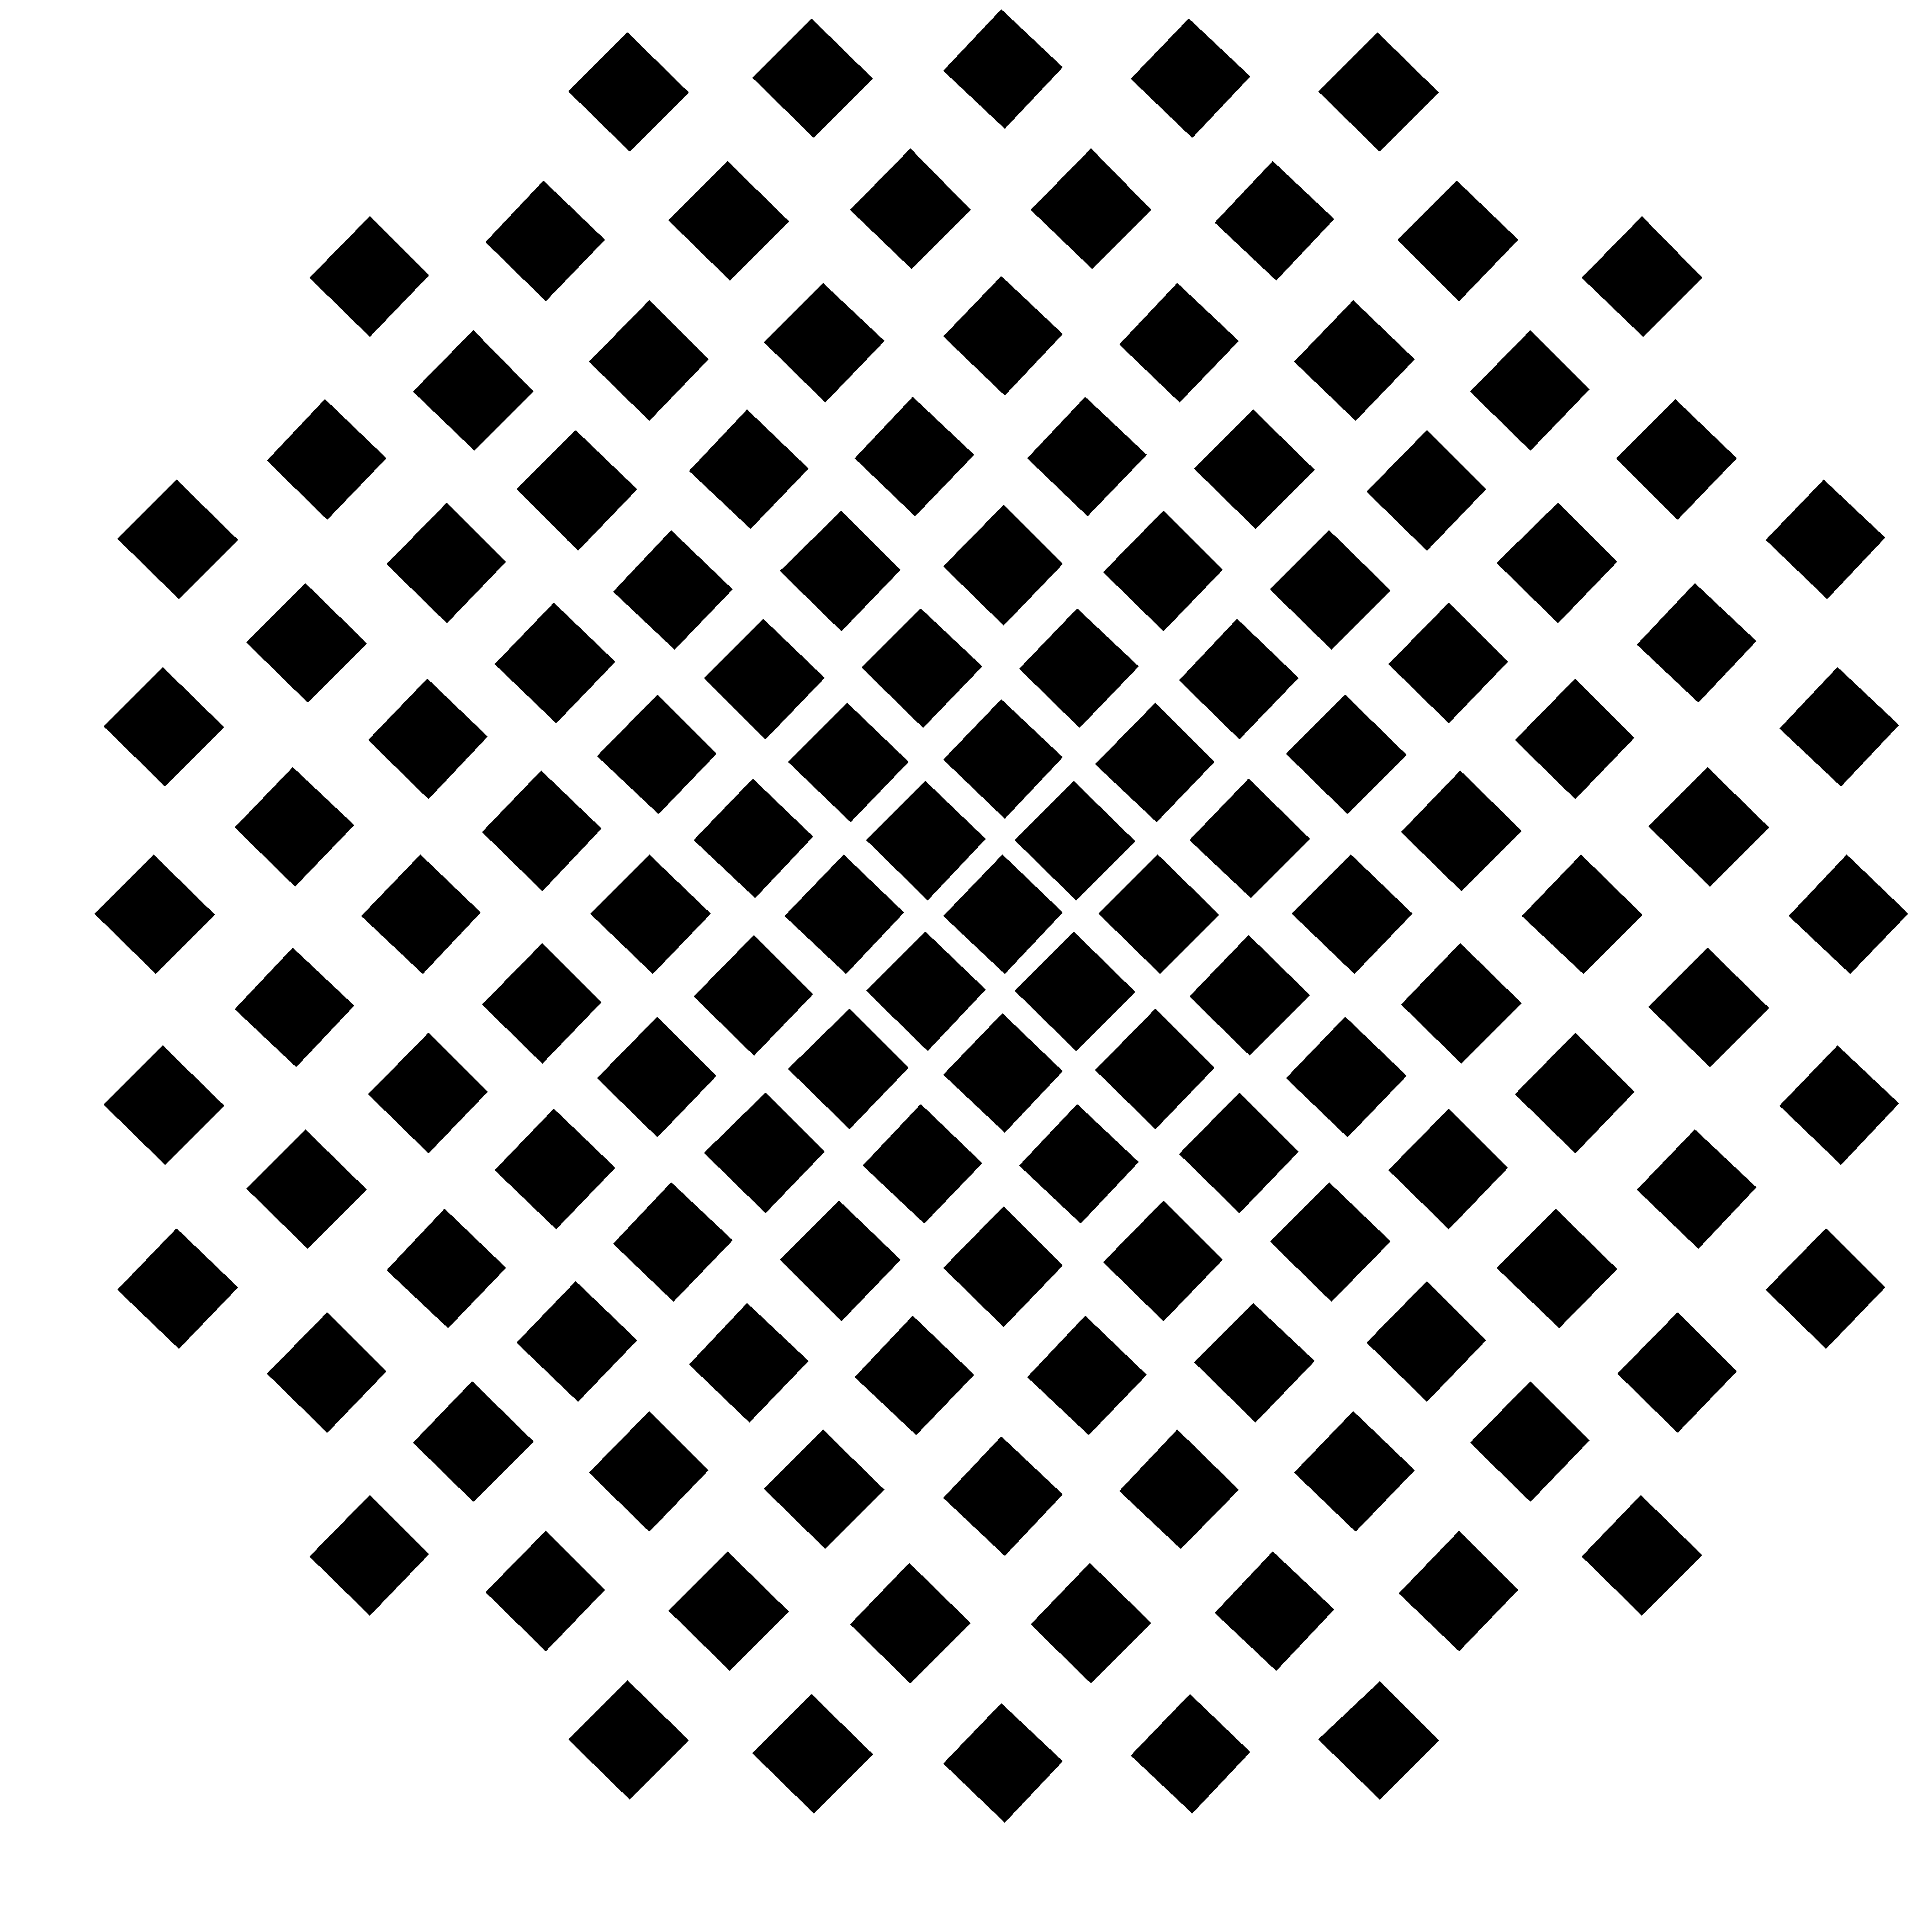
\includegraphics[width=0.9\textwidth]{./gfx/unilogo.pdf}
					%\includegraphics{./gfx/uni_logo.png}
				\end{center}
			\end{minipage}
			\begin{minipage}{3cm}
				\begin{center}
					
\includegraphics{./gfx/iaas.jpg}
				\end{center}
			\end{minipage}
		\end{center}
		%
		\vspace{1.0cm}
		%
		\begin{center}
			\begin{tabular}{ll}
				\textbf{Course of Study:} & Computer Science M.Sc\\
				&\\&\\
				\textbf{Examiner:}   & Prof. Dr. Dr. h. c. Frank Leymann\\
				\textbf{Supervisor:}   & M.Sc. C. Timurhan Sungur\\
				
				\textbf{Commenced:} & 2nd November 2015\\
				\textbf{Completed:}  & \\
				&\\
				\textbf{CR-Classification:} & \\
				
			\end{tabular}
		\end{center}
	\end{sffamily}
\end{titlepage}
%\oddsidemargin=\oddsidemarginorig
%%%%%%%%%%%%%%%%%%%%%%%%%%%%%%%%%%%%%%%%%%%
%Ende Titelblatt
%%%%%%%%%%%%%%%%%%%%%%%%%%%%%%%%%%%%%%%%%%%
	
\cleardoublepage
	
%tex4ht-Konvertierung verschönern
\iftex4ht
% tell tex4ht to create picures also for formulas starting with '$'
% WARNING: a tex4ht run now takes forever!
\Configure{$}{\PicMath}{\EndPicMath}{} 
%$ % <- syntax highlighting fix for emacs
\Css{body {text-align:justify;}}

%conversion of .pdf to .png
\Configure{graphics*}  
         {pdf}  
         {\Needs{"convert \csname Gin@base\endcsname.pdf  
                               \csname Gin@base\endcsname.png"}%  
          \Picture[pict]{\csname Gin@base\endcsname.png}%  
         }  
\fi

%Tipp von http://goemonx.blogspot.de/2012/01/pdflatex-ligaturen-und-copynpaste.html
%siehe auch http://tex.stackexchange.com/questions/4397/make-ligatures-in-linux-libertine-copyable-and-searchable
%
%ONLY WORKS ON MiKTeX
%On other systems, download glyphtounicode.tex from http://pdftex.sarovar.org/misc/
%
\input glyphtounicode.tex
\pdfgentounicode=1

\VerbatimFootnotes %verbatim text in Fußnoten erlauben. Geht normalerweise nicht.

%wird fuer Tabellen benötigt (z.B. >{centering\RBS}p{2.5cm} erzeugt einen zentrierten 2,5cm breiten Absatz in einer Tabelle
\newcommand{\RBS}{\let\\=\tabularnewline}

%% typoraphisch richtige Abkürzungen
\newcommand{\zB}[0]{z.\,B.\xspace}
\newcommand{\bzw}[0]{bzw.\xspace}
\newcommand{\usw}[0]{usw.\xspace}
\renewcommand{\dh}[0]{d.\,h.\xspace}

%from hmks makros.tex - \indexify
\newcommand{\toindex}[1]{\index{#1}#1}
%
\newcommand{\dotcup}{\ensuremath{\,\mathaccent\cdot\cup\,}} %Tipp aus The Comprehensive LaTeX Symbol List
%
%Anstatt $|x|$ $\abs{x}$ verwenden. Die Betragsstriche skalieren automatisch, falls "x" etwas größer sein sollte...
\newcommand{\abs}[1]{\left\lvert#1\right\rvert}
%
%für Zitate
\newcommand{\citeS}[2]{\cite[S.~#1]{#2}}
\newcommand{\citeSf}[2]{\cite[S.~#1\,f.]{#2}}
\newcommand{\citeSff}[2]{\cite[S.~#1\,ff.]{#2}}
\newcommand{\vgl}{vgl.\ }
\newcommand{\Vgl}{Vgl.\ }
%
\newcommand{\commentchar}{\ensuremath{/\mkern-4mu/}}
\algrenewcommand{\algorithmiccomment}[1]{\hfill $\commentchar$ #1}

% Seitengrößen - Gegen Schusterjungen und Hurenkinder...
\newcommand{\largepage}{\enlargethispage{\baselineskip}}
\newcommand{\shortpage}{\enlargethispage{-\baselineskip}}

\pagenumbering{arabic}
%\Titelblatt

%Eigener Seitenstil fuer die Kurzfassung und das Inhaltsverzeichnis
\deftripstyle{preamble}{}{}{}{}{}{\pagemark}
%Doku zu deftripstyle: scrguide.pdf
\pagestyle{preamble}
\renewcommand*{\chapterpagestyle}{preamble}

\setlength{\parindent}{0.0em}


%Kurzfassung / abstract
%auch im Stil vom Inhaltsverzeichnis
%\ifdeutsch
%\section*{Abstract}
%\else
\section*{Abstract}
%State clearly what problem has been studied and/or what is the goal of the %thesis/paper. Give a  brief  statement  on  existing  solutions  and  their  %drawbacks.  List  major  contributions  of  the  thesis.  State  briefly  %assumptions  and  limitations.  The  abstract  should  also  include  major  %idea(s), the type (e.g. performance, complexity) and result of analysis done. 

%\fi
In every field, starting from professional organization to education, human intelligence is one of the most important resource of that field. Despite its importance, it is difficult to systemize them as the human intelligence is something that perceives and acquires differently from human to human. Thus decision making for a similar problem is not going to be the same for every human or for every situations. Informal Process Essentials (IPE) is an approach, proposed to support and automate such unstructured processes. This approach provides neccessary modeling elements to create resource-centric process models. However, an editor to create descriptive models for such processes are still missing. 

Every organization thrives to achieve its intentions, these intentions can be in any levels of  organization like technical intentions that focus to satisfy technical level requirements, management intentions that focus to satisfy the management level requirements, and financial intentions to achieve financial level requirements. Intentions play critical role in many organizations because they motivate organizations towards the overall development. Therefore supporting and automating organizational intentions and associated components are absolute necessary for any organization. In our context, intentions are realized through strategies, which are associated with organizational capabilities, from which resources are created. As a result IPE models are realized as strategy that is associated with capabilities, resources and intentions. The reason for selecting resource-centric organizational modeling is, a process result  may be executed by selecting same set of resources and engaging them towards the intentions of that informal process. 

This Master thesis aims at providing means to design and realize the Resource-centric modeling of organizations. We propose a motivating scenario that helps the reader in easily acquiring the concepts and to validate the usability of developed web editor. The purpose of the web editor is to create/view/update intentions, strategies, capabilities and informal process descriptive models. 


\textbf{Key words:} Informal Process Essentials, Intentions, Capabilities, Strategies and Instances. 

% BEGIN: Verzeichnisse

\iftex4ht
\else
\microtypesetup{protrusion=false}
\fi

%%%
% Literaturverzeichnis ins TOC mit aufnehmen, aber nur wenn nichts anderes mehr hilft!
% \addcontentsline{toc}{chapter}{Literaturverzeichnis}
%
% oder zB
%\addcontentsline{toc}{section}{Abkürzungsverzeichnis}
%\section*{Abkürzungsverzeichnis}
%
%%%

%Produce table of contents
%
%In case you have trouble with headings reaching into the page numbers, enable the following three lines.
%Hint by http://golatex.de/inhaltsverzeichnis-schreibt-ueber-rand-t3106.html
%
%\makeatletter
%\renewcommand{\@pnumwidth}{2em}
%\makeatother
%


\tableofcontents

% Bei einem ungünstigen Seitenumbruch im Inhaltsverzeichnis, kann dieser mit
% \addtocontents{toc}{\protect\newpage}
% an der passenden Stelle im Fließtext erzwungen werden.

%listof* untereinandergesetzt
%ACHTUNG! Falls ein anderer Kapitelstil gewählt wird, muss der Code hier evtl.
%  angepasst werden
\begingroup 
\makeatletter
  \def\@makeschapterhead#1{%
  \vspace*{10\p@}%
  {\parindent \z@ \raggedright \reset@font
            \normalfont \vphantom{\@chapapp{} \thechapter}
        \par\nobreak\vspace*{10\p@}%
        \interlinepenalty\@M
    {\huge \bfseries %
    %
    %Default-Schrift: Serifenhaft (fuer englische Dokumente)
    % Dann sowohl A als auch B deaktivieren
    %A) Fuer serifenlose Schrift folgende Zeile aktivieren:
    \ifdeutsch
    \fontfamily{phv}\selectfont
    \fi
    %B) Fuer Kapitaelchen folgende Zeile aktivieren:
    %\fontseries{m}\fontshape{sc}\selectfont
    %
    #1\par\nobreak}
    %\vspace*{1\p@}%
\makebox[\textwidth]{\hrulefill}%    \hrulefill alone does not work
    \par\nobreak
    \vskip 5\p@
  }}
\makeatother
\cleardoublepage
\listoffigures
%\cleardoublepage
%\newpage
%\let\cleardoublepage\relax
\cleardoublepage
\listoftables

%\newpage
%Wird nur bei Verwendung von der lstlisting-Umgebung mit dem "caption"-Parameter benoetigt
%\lstlistoflistings 
%ansonsten:
\cleardoublepage
\ifdeutsch
\listof{Listing}{List of Listings}
\else
\listof{Listing}{List of Listings}
\fi

%mittels \newfloat wurde die Algorithmus-Gleitumgebung definiert.
%Mit folgendem Befehl werden alle floats dieses Typs ausgegeben
%\ifdeutsch
%\listof{Algorithmus}{List of Algorithms}
%\else
%\listof{Algorithmus}{List of Algorithms}
%\fi
%\listofalgorithms %Ist nur für Algorithmen, die mittels \begin{algorithm} umschlossen werden, nötig

\endgroup

\cleardoublepage

\iftex4ht
\else
%Optischen Randausgleich und Grauwertkorrektur wieder aktivieren
\microtypesetup{protrusion=true}
\fi

% END: Verzeichnisse


\renewcommand*{\chapterpagestyle}{scrplain}
\pagestyle{scrheadings}
\pagestyle{scrheadings}

%ihead aufgeteilt - Bezeichnungen: 4.1, S. 119, scrguide

%für die Teilversionen - nur bei Verwendung von RCS/CVS
%\ihead[Version \RCSRevision]{Version \RCSRevision}

%Für die finale Version oder bei Verwendung von SVN
\ihead[]{}


% Sowohl für die Teilversionen als auch die finale Version:

\chead[]{}
\ohead[]{\headmark}
%
\cfoot[]{}
\ofoot[\usekomafont{pagenumber}\thepage]{\usekomafont{pagenumber}\thepage}
\ifoot[]{}

%
%
% ** Hier wird der Text eingebunden **
%
\cleardoublepage
\chapter{Introduction}
\label{chap:introduction}
\begin{center}
	\textit{Creating a better world requires teamwork, partnerships, and collaboration, as we need an entire army of companies to work together to build a better world within the next few decades. This means corporations must embrace the benefits of cooperating with one another -  Simon Mainwaring}
\end{center}

 Every organization knows the benefits of collaborating a process in order to achieve its desired intention. Resources of an organization play an important role to collaborate and accomplish those tasks. Though organizations re-use data resources and tool resources during this collaboration work, business logics and decisions cannot be reused in certain types of processes. These type of processes are not structured like traditional processes because the process execution steps cannot be pre-defined due to its dynamic nature e.g processes that require involvement of human knowledge in deciding the execution steps. Such type of processes are called \textit{Informal Processes} \cite{Sungur2014}.

Humans play an important role in informal processes which makes the informal processes collaborative in nature. The participants of an informal processes collaborate to accomplish a task. These participants are the resources that drives towards the accomplishment of the task.  Developing an editor to create models for such \textit{resource-centric informal processes} is a part of realizing the automated execution of informal processes. In this document, we explain how we realized developing an editor that creates models for resource-centric informal processes. Along with this we also validate the developed prototype using a case study. This case study has been taken as an example scenario throughout this document that helps for better understanding of the concepts.

In this Chapter, the first section provides a detailed motivational reasons about why this work is relevant and what about this work is new.  The second section contains an overview about the problems in existing approaches and how this approach serves as an \textit{complemenatry approach} to the existing work. The third section discusses about the contributions done in this work i.e., the research objectives satisfied by this approach. The final section provides an overview about the following chapters. 

%%%%%%%%%%%%%%%%%%%%%%%%%%%%%%%%%%%%%%%%%%%%%%%%%%%%%%%%%%%%%%%%%%%%%%%%%
\section{Motivation}
\label{sec:motivation}
%%%%%%%%%%%%%%%%%%%%%%%%%%%%%%%%%%%%%%%%%%%%%%%%%%%%%%%%%%%%%%%%%%%%%%%%%
Nowadays, any task has both well defined predictable elements and less defined ambiguous elements. In tasks with less defined ambiguous elements, knowledge workers' decision plays an important role\footnote{White, Michael. "Case management: Combining knowledge with process." BPTrends, July (2009).}. For example, research and development projects are of type where \textit{what to do next} cannot be decided much in advance. These type of processes are highly unpredictable in nature and this makes it quite challenging to support and automate these type of processes. This work is a part in realizing the automation of such processes. These \textit{unstructured/informal/human-centric processes} are called as \textit{informal processes} \cite{Sungur2014}. Any approach that supports informal process automation is required to be more autonomous because of their dynamic behavior of enacting a process, so the existing approaches available for traditional processes are not helpful in realizing the execution of informal processes.  

Though the execution steps of informal processes cannot be determined beforehand, \textit{intentions} of informal processes are known before their enactment \cite{Sungur2015}. Achieving these intentions requires another important driving force called \textit{resources}. Resources can be anything from human actors, development environment, materials etc. These resources posses certain \textit{capabilities} to qualify for achieving an intention. So we need an approach that supports informal processes along with the support of intentions, resources, capabilities etc. This can be achieved by associating intentions with strategies, strategies with capabilities and capabilities with resources. Sungur et al. \cite{Sungur2014a} provided a descriptive meta-model approach called \textit{Informal Process Essentials}. This work serves as a part of the work by Sungur et al. Also, this work focuses to provide a web based editor to create resource-centric models of organizations. The reason for selecting descriptive modeling approach is to preserve the essential information associated with informal processes such as intentions, context information, resource definitions etc.  This work also provides means to initialize and acquire instances which can be further extended during enactment of resource-centric informal processes.  

The developed editor serves as an \textit{descriptive} web based editor tool, where the business experts can create models for informal processes, intentions, strategies, capabilities etc and this work does not comprise any functionality for compiling and executing the models. Instead this editor provides facility to plug-in the functionality for transforming the descriptive information of the models into deployable information. 

%%%%%%%%%%%%%%%%%%%%%%%%%%%%%%%%%%%%%%%%%%%%%%%%%%%%%%%%%%%%%%%%%%%%%%%%%
\section{Problem Statement}
\label{sec:problemstatement}
%%%%%%%%%%%%%%%%%%%%%%%%%%%%%%%%%%%%%%%%%%%%%%%%%%%%%%%%%%%%%%%%%%%%%%%%%
 Every organization contains multiple entities like \textit{resources} e.g., humans, tools etc., \textit{intentions} e.g., revenue based intentions, quarterly intentions etc., \textit{strategies} e.g., the process to achieve the intention and \textit{capabilities} e.g., a resource that can provide a particular capability. Thus an organization needs efficient mechanisms to handle and manage these different types of entities. Informal processes are collaborative in nature, which means that participants of informal process collaborate with each other to accomplish its intentions\cite{Sungur2015}. Designing these collaborations and assigning participants their respective privileges, plays an important role during modeling of the respective informal processes. The research work by Matthews et. al \cite{Matthews2011} mentions that below points are the major problems in adopting to a workspace collaboration tools.

\begin{enumerate}
	\item Lack of Methods
	\item Methods that focus on individuals
	\item Not well targeted groups
	\item Not well supported editors for executing abstract descriptions
\end{enumerate}

Though there are \textit{activity-centric} modeling and reusing of business processes such as Business Process Execution Language (BPEL) \footnote{http://docs.oasis-open.org/wsbpel/2.0/OS/wsbpel-v2.0-OS.pdf} and Business Process Model and Notation (BPMN) \footnote{http://www.omg.org/spec/BPMN/2.0/PDF/} are available, they are not suitable for certain type processes whose execution steps cannot be predicted in advance \cite{Sungur2014a}. Also complementary concepts such as automatic initialization and acquiring of interrelated resources are still missing in the existing work \cite{Sungur2015}. Another key thing to remember is informal processes are volatile in nature which is one of the important challenges in developing an environment that supports informal processes.

%%%%%%%%%%%%%%%%%%%%%%%%%%%%%%%%%%%%%%%%%%%%%%%%%%%%%%%%%%%%%%%%%%%%%%%%%
\section {Research Objectives}
\label{sec:researchobjectives}
%%%%%%%%%%%%%%%%%%%%%%%%%%%%%%%%%%%%%%%%%%%%%%%%%%%%%%%%%%%%%%%%%%%%%%%%%
The main focus of this work, is to realize the phase \textit{Informal Process Modeling} (P2) described in \textit{Executing Informal Processes} (InProXec) approach \cite{Sungur2015}. Coupled with the main focus of developing web based editor, the following research objectives provided in the Table \ref{tab:researchobjectives} are also satisfied by the developed editor. 

\label{sec:researchobj}
\begin{center}
	\begin{longtable}{p{5cm}p{11cm}} 
   	\toprule 
	\textbf{Research Objectives} & \textbf{Description} \\
	\midrule
	\endfirsthead
	\\
	R1 & \textit{Organizational intentions transparency}  \label{ro1} \\
	\\[-1.5ex]
	R2 & \textit{Organizational intention resource-based cost estimation}  \label{ro2} \\
	\\[-1.5ex]
	R3 & \textit{Organizational intention achieve-ability estimation} \label{ro3}\\
	\\[-1.5ex]
	R4 & \textit{Intention oriented working style}  \label{ro4}\\
	\\[-1.5ex]
	R5 & \textit{Participative organizational modeling}\label{ro5}\\
	\\[-1.5ex]
	R6 & \textit{Re-use of organizational knowledge} \label{ro6}\\	
	\bottomrule
	\caption{Research Objectives}
	\label{tab:researchobjectives}
	\end{longtable}	
\end{center}

%%%%%%%%%%%%%%%%%%%%%%%%%%%%%%%%%%%%%%%%%%%%%%%%%%%%%%%%%%%%%%%%%%%%%%%%%
\section {Outline}
\label{sec:outline}
%%%%%%%%%%%%%%%%%%%%%%%%%%%%%%%%%%%%%%%%%%%%%%%%%%%%%%%%%%%%%%%%%%%%%%%%%
The remainder of this document is organized into following chapters:
\begin{description}
	\item[Chapter ~\ref{chap:fundamentals} -- \nameref{chap:fundamentals}:] In this chapter, basic fundamental concepts and an overview of the related approaches that are essential to understand the work are provided.
	\item[Chapter ~\ref{chap:motivatingScenario} -- \nameref{chap:motivatingScenario}:] In this chapter, a motivating scenario has been taken and detailed explanation for each phases of the scenario has been provided. This aids the reader to understand the concepts of organizational modeling clearly. 
	\item[Chapter ~\ref{chap:analysis} -- \nameref{chap:analysis}:] This chapter provides detailed requirement analysis based on scientific facts published in existing works. This chapter also provides literature review of existing works.
	\item[Chapter ~\ref{chap:approach} -- \nameref{chap:approach}:] This chapter discusses about the methodology followed in realizing the concepts  of resource-centric organizational.
	\item[Chapter ~\ref{chap:casestudy} -- \nameref{chap:casestudy}:] This chapter validates the approach presented in Chapter \ref{chap:approach}. This chapter also discusses detailed system architecture and also presents the validation results. The abstract concepts motivating scenario discussed in \ref{chap:motivatingScenario} is explained in a concrete way.	
	\item[Chapter ~\ref{chap:conclusion} -- \nameref{chap:conclusion}:] This chapter summarizes the results of the work and draws conclusion. This chapter also throws some light on the future work to be carried out in the approach of executing informal processes. 
\end{description}
\cleardoublepage
\chapter{Fundamentals and Related Work}
\label{chap:fundamentals}
This chapter provides the fundamental concepts and related work that are required to understand the approach to be discussed in following Chapter \ref{chap:approach}. The first section introduces definitions of terms that are used throughout this document. The second section provides a brief introduction about the Informal Process Essentials (IPE) approach, as this provides basic information required for understanding this thesis work. The third section provides a short overview about organizational modeling notations mentioned in a thesis work \cite{Sierr2015}. Though provided notations are not part of implementation, it is introduced to assist the reader in better understanding. The fourth section also describes about fundamental information required to understand the concepts of this thesis work. The fifth section discusses about the entity types representation of the organizational modeling. The last section discusses in details about each steps of the informal process modeling phase. 

%%%%%%%%%%%%%%%%%%%%%%%%%%%%%%%%%%%%%%%%%%%%%%%%%%%%%%%%%%%%%%%%%%%%%%%%%
\section{Definitions of Terms}
\label{sec:termdefinitions}
%%%%%%%%%%%%%%%%%%%%%%%%%%%%%%%%%%%%%%%%%%%%%%%%%%%%%%%%%%%%%%%%%%%%%%%%%
In this section, the definitions of terminologies that are used throughout this document are provided briefly.

\textit{Business Process} -  A business process has been defined as the set of activities whose final output is accomplishment of a goal \cite{Weske2012}.  

\textit{Business Logic} - Business logic refers to the activities that need to be done to execute the corresponding process. 

\textit{Business Process Models} - Business process models are models to capture recurring activities during a business process execution and enact them in a automated fashion for re-using those stored knowledge. 

\textit{Informal Process} - Informal processes are the processes whose execution steps cannot be modeled or are not feasible to model before their enactments. This is because due to the dynamic changing behavior during execution of the informal processes.  For example, software development process is an informal process, where required activities and order of their execution cannot be determined beforehand \cite{Sungur2015}.    

\textit{Informal Process Essentials} - Informal Process Essentials (IPE) is a resource-driven approach that enables describing process declaratively, i.e., without describing how the intention is achieved, and providing only information about what has to be achieved \cite{Sungur2014a}. 

\textit{OASIS Topology and Orchestration Specification for Cloud Applications} (TOSCA) - TOSCA  is  a  new  OASIS (Organization for the Advancement of Structured Information Standards)  standard  to  describe  composite applications  and  their  management \cite{Kopp2013}.  

\textit{Winery} - Winery is a modeling tool offering an HTML5-based environment for graph-based modeling of application topologies and defining reusable component and their relationship types. It uses TOSCA as an internal storage, import, and export format \cite{Kopp2013}. 
 
%%%%%%%%%%%%%%%%%%%%%%%%%%%%%%%%%%%%%%%%%%%%%%%%%%%%%%%%%%%%%%%%%%%%%%%%%
\section{Overview of Informal Process Essentials}
\label{sec:basicconcepts}
%%%%%%%%%%%%%%%%%%%%%%%%%%%%%%%%%%%%%%%%%%%%%%%%%%%%%%%%%%%%%%%%%%%%%%%%%
In this section, we provide an overview about the concepts introduced in the approach Informal Process Essentials (IPE) \cite{Sungur2014a}. The execution steps of a process are recorded as models. These models can be represented as graphs, linguistic description, etc. Models are used in various fields like manufacturing, scientific, IT, etc. These models are mainly useful in re-using the predefined solutions. Such models have numerous benefits \footnote{http://www.nomagic.com/getting-started/modeling-benefits.html} like performance improvement, reduced cost of operation and design, etc. Besides the traditional processes, there are processes which requires participation of human. The performance of these processes depend on dynamic nature of human knowledge i.e., they are subject to change and carried out based on experience of previous knowledge. 

The authors describe following as the properties of an informal process (1) business logic of informal processes is not defined explicitly before the enactment, (2) informal processes are collaborative in nature which requires resources with interrelationships (3) a resource can participate in multiple informal processes and (4) resources can change dynamically.

The authors also suggest following requirements that support informal processes with the above described properties. The summarized requirements are (1) ability to represent informal process as models and ability to execute it, (2) due to involvement of multiple resources, ability to define relationships among the resources, (3) resources should be visible in process representations and (4) support for dynamically changing resources. 

The authors also compare existing approaches in the literature with the above requirements. It has also been concluded that analyzed approaches only satisfies some of the requirements but not all the requirements completely. So the author proposes a new \textit{meta-model} approach that satisifies all the requirements. In this IPE meta-model approach, resources are related to each other and work towards achievement of an intention i.e., goal.   

This thesis work also realizes the concept of \textit{resource-centric modeling of informal processes}, specified in the Informal Process Essentials (IPE) \cite{Sungur2014a}.  As mentioned in Section \ref{sec:termdefinitions}, resources are drivers to achieve intentions in the informal processes. In the IPE approach, author states that when the desired process result is repeated the same set of resources can be selected and engaged towards collective intention of the informal processes. 
 
It has been mentioned in the IPE approach that Informal Process Essentials (IPE) meta-model describes the following about informal process: (1) describes the constituents informal process such as performers, data and software tools and (2) describes how to make core element ready for the enactment of the informal process i.e resource providers. IPE models begin from initial context and after achieving the main intention it results in another context. 

%%%%%%%%%%%%%%%%%%%%%%%%%%%%%%%%%%%%%%%%%%%%%%%%%%%%%%%%%%%%%%%%%%%%%%%%%
\section{Human Centric Process}
\label{sec:humancentric}
%%%%%%%%%%%%%%%%%%%%%%%%%%%%%%%%%%%%%%%%%%%%%%%%%%%%%%%%%%%%%%%%%%%%%%%%%
The role of humans in organizations has been evolving over time. The shift from "personnel" to "human resources" acknowledges the importance of humans as organizational resources. There are incredible number of pressure on today's organizations \footnote{http://www.siop.org/tip/backissues/tipjan98/may.aspx} due to dynamic nature of organizations. For example, organizational changes like addition of new organizational alliances, new structures and hierarchies, new ways of assigning work, and a very high rate of changes like changes in the workforce, including employees' priorities, capabilities, and demographic characteristics. Thus it is impossible to do one hundred percent perfect forecasting of dynamically changing processes in an organization.

In order to manage such a dynamic environment, organizations need skilled human resources with previous knowledge of handling unforeseen scenarios. Thus human resources are vital part of any organizations as they have skills of acute future orientation to understand changing organizational environment. Humans in organizations carry out many important activities. Managers and Human Resource (HR) professionals organize jobs of each and every human in the organization so that they can effectively perform these jobs. Thus humans in any organization are viewed as resources of the organization which is a contemporary part of Human Resource Management \footnote{http://smallbusiness.chron.com/role-human-resource-management-organizations-21077.html}.

When there are multiple human resources working for a process, then there should be some sort of co-ordination and understanding between the humans which is called \textit{collaboration} at an organizational level. Collaboration exists in every levels of an organization. For example at management levels of an organization, managers and HR professionals work together to assign employees their roles and task in the organization. This helps the employees of the organization to adapt to its environment. In a flexible organization, employees' roles and responsiblities changes dynamically based on the requirements and business priorities. Thus the need for network of representations between the human resources arising. This network of representation sets up an environment to support collaborative work of business related process. This kind of support to represent human resource network has been realized in the work by author Canko \cite{Canko2015}. The concept of \textit{virtual human representation} described by author \cite{Canko2015} is an extension of actor-concept described in \textit{Informal Process Essentials} \cite{Sungur2014a}. The developed prototype \textit{Human Resource Representation} in the work by the author Canko\cite{Canko2015} saves the information such as capabilities, roles, responsibilities etc.  as a virtual human web ontology instance which can be re-used in web based environments.

These kind of human representation are highly helpful to organizations with dynamically changing resources. These representations can describe and match resources with their capabilities based on the requirements. As we have mentioned in Chapter \ref{chap:introduction}, in our context of resource-centric modeling humans are also considered as resources and we associate \textit{capabilities} with every resources. Moreover, associating capabilities with resources is helpful in the following example situation. For example, there can be a situation where resources producing more accurate results for a processing task are preferred than resources which can produce higher throughput for a processing task. Thus we need to associate capabilities with each resources and need to automate the process of discovering and matching the resources with their capabilities based on their process. 

%%%%%%%%%%%%%%%%%%%%%%%%%%%%%%%%%%%%%%%%%%%%%%%%%%%%%%%%%%%%%%%%%%%%%%%%%
\section{Organizational Modeling Notations}
\label{sec:resourcecentricorganizationalmodeling}
%%%%%%%%%%%%%%%%%%%%%%%%%%%%%%%%%%%%%%%%%%%%%%%%%%%%%%%%%%%%%%%%%%%%%%%%%
The organizational modeling element notation has been selected as per the guidelines mentioned in the literature \cite{Moody2009} and these notations are taken from a thesis work \cite{Sierr2015}. Though these notations modeling are not part of this master thesis, this has been provided in this section for the sole purpose of aiding the reader to understand the concepts much better through pictorial representations. Also by observing  the fact that business process modelers are already well-known with the present process modeling notations such as Business Process Modeling Notation 2.0 (BPMN) \cite{bpm2011} and ArchiMate notation\cite{arc2013}, the shape depiction of organizational model elements has been designed similar to those existing process notations. 

Due to the importance of shapes in expressing information visually \cite{Moody2009}, the notations are chosen in such a way that each element of organizational modeling  differ by shape. Also a legend will be always shown in the modeling notation to denote the meaning of each shape. The description of each element in the organizational model notation is shown in the Table \ref{tab:notations}. 

\begin{center}
	\begin{longtable}{p{3cm}p{10cm}p{3cm}}
		\toprule 
		\textbf{Element} & \textbf{Definition} & \textbf{Notation} \\
		\midrule
		\endfirsthead
		Intentions 			& Intentions are purposeful concrete steps taken by organizations or individuals to achieve an expected outcome. & \begin{center} 
\includegraphics[width= 0.07\textwidth]{Intention.pdf}  \end{center}  \\
		
		Capabilities	&  Capability is an ability that should be possessed by a resource that work towards achievement of one or several intentions.   & \begin{center} 
\includegraphics[width= 0.07\textwidth]{Capability.pdf} \end{center}  \\
		
		Context				& The environment that forms the setting for an event, statement, or idea and in terms of which it can be fully understood. There are two Contexts: initial and final. Initial context is the situation which describes the driving forces that trigger the process to start. Final context is the expected situation once the process has finished. Both initial and final context are represented by an hexagonal shape except the final context has thick edges than initial context.  & \begin{center} 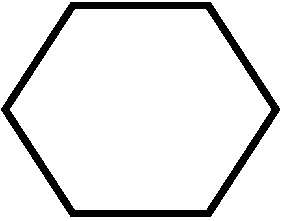
\includegraphics[width= 0.07\textwidth]{Context.pdf} \end{center}   \\
		\newline
		Strategy		& \newline  A method or plan chosen to bring about a desired future, such as accomplishment of an intention.   & \begin{center} 
\includegraphics[width= 0.07\textwidth]{Strategy.pdf} \end{center}  \\
		
		Resources					& The people or tools those/that needed to fulfill the middle objectives or work towards the achievement of intentions . & \begin{center} 
\includegraphics[width= 0.07\textwidth]{Resource.pdf} \end{center}  \\
		
		Relationship				& A relationship is used specify the fixed links between the elements of the model.  & \begin{center} 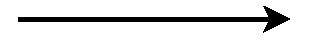
\includegraphics[width= 0.07\textwidth]{Relationship.pdf} \end{center}   \\
		
		\bottomrule
		\caption{Organizational Modeling Notations}
		\label{tab:notations}		
	\end{longtable}	
\end{center}


%%%%%%%%%%%%%%%%%%%%%%%%%%%%%%%%%%%%%%%%%%%%%%%%%%%%%%%%%%%%%%%%%%%%%%%%%
\section{Intention-oriented Organizational Modeling - Conceptual Model}
\label{sec:entitytypesrepresentation}
%%%%%%%%%%%%%%%%%%%%%%%%%%%%%%%%%%%%%%%%%%%%%%%%%%%%%%%%%%%%%%%%%%%%%%%%%
The conceptual model of entity types in organizational modeling is shown in Figure \ref{fig:entitymodel}. This model shows that among all the entity types, intentions are in the top level of hierarchy which can be further divided into \textit{strategies}. An intention can either contradict or be a sub intention of another intention. These type of sub-intention and contradicting intention has been explained in detail with a suitable example in Chapter \ref{chap:motivatingScenario}.  An intention can be achieved through a strategy, which is a plan of action designed to meet the intention. An intention can be achieved through none or many strategies. Strategies also describe none or many capabilities and processes required to achieve intention. The capabilities and processes can be further resolved into resources or resource models. Thus starting from defining intentions, we define strategies then required capabilities and process models. The capabilities and process models define the required resources. 

Organizational process modeling of this approach is a \textit{intention-oriented} approach as they support processes by providing required resources and thrives to successfully execute the processes by using qualified autonomous agents, i.e., actors under certain \textit{context definitions}.  As we mentioned before, in our context resources can be anything like people, IT tools, data that are used to accomplish the objectives. Emerging intentions can result in the requirement of new capabilities, i.e., resources. Resource models are also provided in the developed prototype to make precise definitions of resources needed.

\begin{figure}
	\centering
	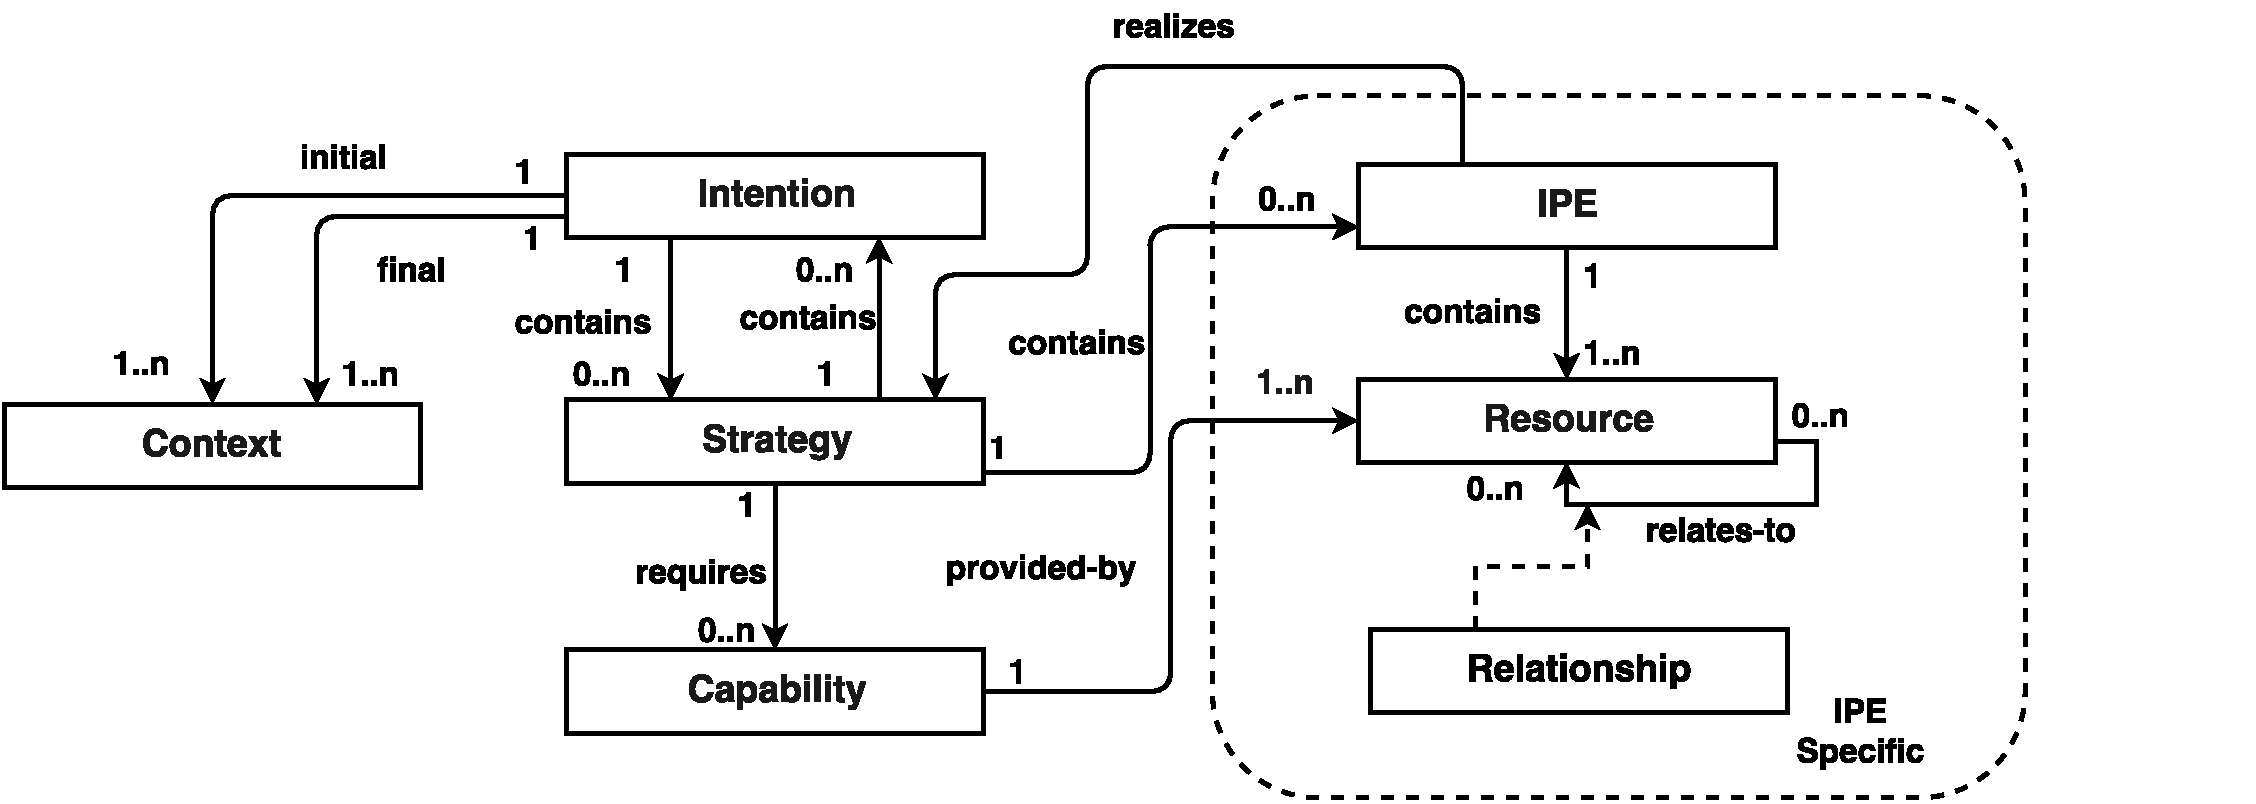
\includegraphics[width=1.1\textwidth]{entity.pdf}
	\caption{Intention-oriented Organizational Modeling: Conceptual Model}
	\label{fig:entitymodel}
\end{figure}

In Sungur et al \cite{Sungur2014a} work, the concept of \textit{Informal Process Support Model} (IPSM) has been introduced which is to make use of existing knowledge of human performers. Here the initial creator of the model is experienced human performers. Based on their experience, they add relevant  resources of an informal process. The models are generated at runtime based on the interactions and activities of corresponding human performers. An informal process targets for accomplishment of an intention. The intentions can be refined by defining sub-intentions and/or strategies, which can then be further refined recursively as independent informal processes. The intention-based approach enables describing processes declaratively, i.e., without describing \textit{how} the intention is achieved, and providing only information about \textit{what} is achieved. As the author \cite{Sungur2014a} suggests that this avoids need of predefined business logic in the representations of informal processes. Each resource can be related to another resource in the context of an informal process using predefined or custom \textit{Relationships}. Informal Process Essentials are realized through strategies. Each informal process starts from an initial context, i.e., \textit{initial context} and aims to achieve an intention. After accomplishing the intention, there is a resulting context called as \textit{final context}. The beginning state before achieving intention is called as initial context and the end state after achieving intention is called as final context. On completion of intention execution, the process state changes from one state to another.

%%%%%%%%%%%%%%%%%%%%%%%%%%%%%%%%%%%%%%%%%%%%%%%%%%%%%%%%%%%%%%%%%%%%%%%%%
\section{Second Phase of InProcXec}
\label{sec:inproxec}
%%%%%%%%%%%%%%%%%%%%%%%%%%%%%%%%%%%%%%%%%%%%%%%%%%%%%%%%%%%%%%%%%%%%%%%%%
In this section, we present an overview about the \textit{Executing Informal Processes} (InProXec) method, proposed by Sungur et al. \cite{Sungur2015}. Implementing IPE approach in organization requires the application of InProXec with different phases. The InProXec method enables modeling of informal processes and automated provisioning of resources modeled in these processes. Since this thesis work is realizing intention-oriented modeling of organizations, the main focus of this section is on the second phase of InProXec which is \textit{Informal Process Modeling}(P2). The method described in Figure \ref{fig:inprocxec_steps}, initializes informal process models in an automated fashion. The author also proves feasibility of the approach with a suitable case study.  In the following paragraphs, a short overview about different phases of the InProXec method has been provided and with a detailed description about the second phase of the \textit{InProXec} method. 

\begin{figure}
	\centering
	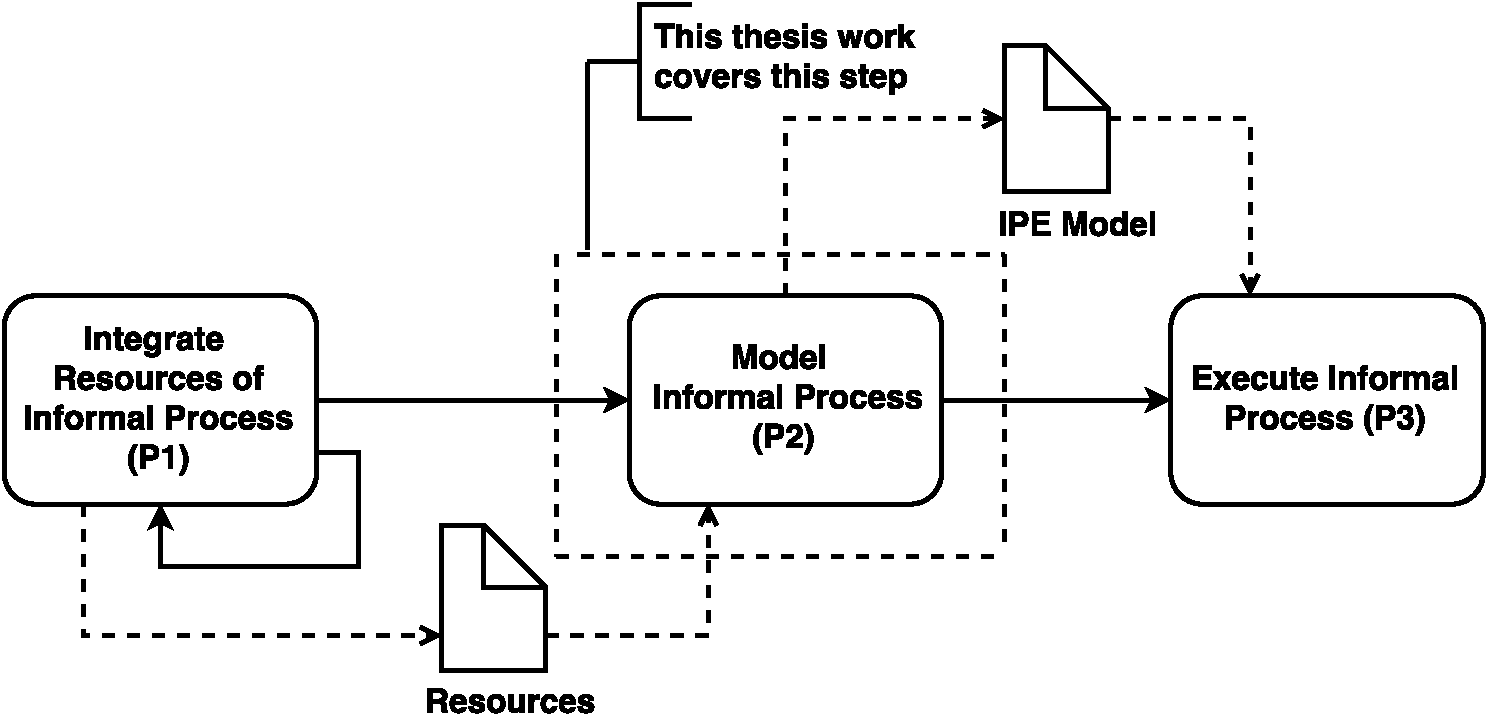
\includegraphics[width= \textwidth]{InProXec_Steps.pdf}
	\caption{Steps of the InProXec approach \cite{Sungur2015}}
	\label{fig:inprocxec_steps}
\end{figure} 

As shown in the Figure \ref{fig:inprocxec_steps}, the InProcXec method consists of three different phases:


Therefore, technical experts develop execution environment integrators  capable of allocating resource defintiions
Included in the informal process models. After this phase, business experts can create informal process models 
Using the resources provided and initizialization of these models happens automatically using execution environment integrators


\textit{Integrate Resources of Informal Processes (P1)} - The first phase aims for creating the required infrastructure to enable modeling and automated initialization of informal processes. This is because modeling tools of informal processes need to present business experts  all
resource definitions important for informal processes of the respective organization. The required resource definitions for an informal process are allocated by \textit{execution environment integrators} developed by technical experts. The final output of this phase is \textit{resources definitions} which are used by next phase P2. 

\textit{Model Informal Processes (P2)} - This phase receives resource definitions made available in the first phase P1 as an input.  Based on this, business experts model informal processes. This phase has been explained in detail in the following sub-section \ref{subsec:informalprocessmodeling} of Chapter \ref{chap:approach}

\textit{Execute Informal Processes (P3)} - Initialization of models developed in phase P2 happens automatically using execution environment integrators developed in phase P1. In phase P2, the functionality to instantiate acquirable entities are not included. Thus in third phase P3, the output of phase P2 is taken i.e IPE models and are transformed into initialize-able self-contained \textit{Deployable Informal Process Essentials Archives(DIPEA)} \cite{Sungur2015} takes place. This results in DIPEAs enacting required informal process. To realize, phase P3 an \textit{IPE Model Compiler} also been introduced in the approach. Additionally, this phase also employs \textit{IPE Runtime} which parses DIPEAs and runs the executables contained in those archives. During this phase, the autonomous actors work towards intentions of informal processes using acquired resources and other involved resources.  












\cleardoublepage
\chapter{Motivating Scenario}
\label{chap:motivatingScenario}

In order to help in understanding the concepts of organizational modeling, the below motivating scenario has been taken and explained through the notations mentioned in Section \ref{sec:resourcecentricorganizationalmodeling}. This scenario also helps in validating the developed web editor in Chapter \ref{chap:casestudy}. The motivating scenario has been chosen based on the collected real life scenarios provided in the thesis work \cite{Sierr2015}. The scenario of this example was taken from the context of manufacturing sector. The main intention of the organization in this scenario is \textit{to increase the quarterly revenue and number of unit sales}. In order to achieve this main intention through our organizational modeling approach, as a first step we need to break the intention from abstract level into concrete levels like strategies, sub-intentions, process definitions, resource definitions etc. This intention can be achieved by following all of the below mentioned strategies, which requires resources with matching capabilities.  
\begin{enumerate}
	\item Increasing the revenue through expanding the market sales. 
	\item Through improving the excellence of the product which in turn brings back old and new customers.
	\item Through increasing the advertisement which helps in customer knowing about the product.
\end{enumerate}

In this chapter, the first section provides an overview about the motivating scenario followed by second section that explains in detail about the motivating scenario. The third section provides an abstract overview about the entity types in the motivating scenario which will be explained in a concrete way, in the following Chapter \ref{chap:casestudy}.

%%%%%%%%%%%%%%%%%%%%%%%%%%%%%%%%%%%%%%%%%%%%%%%%%%%%%%%%%%%%%%%%%%%%%%%%%
\section{Overview of Motivating Scenario}
\label{sec:overview}
%%%%%%%%%%%%%%%%%%%%%%%%%%%%%%%%%%%%%%%%%%%%%%%%%%%%%%%%%%%%%%%%%%%%%%%%%
The motivating scenario provided in this chapter serves as a running example throughout this document, to help the reader in understanding the concepts better. We have taken a scenario of laptop manufacturing company, where the \textit{main intention} of the organization in current context is to increase the revenue of the company. The participating resources work towards one \textit{main intention} and certain \textit{sub-intentions}. Sub-intentions are part of main intention, which helps the resources to modularize and achieve the main intention. Also each sub-intention has certain type of relationship with main-intention. For example in our below described motivating scenario in Section \ref{sec:scenario} one of the sub-intention is to \textit{expand sales geographically} . Before executing this sub-intention, few ground works like collection of laptop usage statistics such as average buying capacity of the consumers, average computer knowledge in the new area has to be done. Thus the execution of main intention i.e \textit{increase revenue and number of unit sales}, requires collaboration of people with different skills and expertise. People who has skills to collect and study statistics can serve as external resources. As new intentions may emerge dynamically the team working towards the achievement of main intention should also be ready to accommodate new resources with new capabilities and skills. There is also a software development team, which work towards achievement of one of the sub-intention \textit{improve help desk}, i.e this team develops software that automatically attends and records user queries.  The management of the project is done through the support of project management software called Redmine \footnote{http://www.redmine.org/}. The participating human resources are members of business oriented social network called XING \footnote{http://www.xing.com/}.
 


%%%%%%%%%%%%%%%%%%%%%%%%%%%%%%%%%%%%%%%%%%%%%%%%%%%%%%%%%%%%%%%%%%%%%%%%%
\section{Resource-centric Organizational Modeling Example}
\label{sec:scenario}
%%%%%%%%%%%%%%%%%%%%%%%%%%%%%%%%%%%%%%%%%%%%%%%%%%%%%%%%%%%%%%%%%%%%%%%%%
 The concept of resource centric organizational modeling can be explained with the following scenario in a manufacturing organization. ABC Ltd. is a budding computer technology company which designs, develops, manufactures and sells personal computers, tablets and laptops. The CEO's intention of the quarter is to increase the revenue and number of unit sales. The initial context describes the situation before starting the execution of intention. The initial context also provides description that motivates to start the process. The final context describes the situation that is achieved once the intention executed successfully. Intentions connect initial context definitions with final context definitions \cite{Sungur2014a}. The sub-intentions are the intermediate intentions which describes the expected outcome in a measurable form. Intentions reach strategy implementations through achieving strategies which are plans of action designed to meet a specific intention. 

 The example scenario ABC Ltd. follows top-down approach of organizational modeling i.e., how organization's higher level intentions can be achieved by amalgamation of specific, measurable and realistic sub-intentions, strategies etc. The whole view has been divided into Intention view and Strategy view. The \textit{Intention View} shown in the Figure\ref{fig:motivatingscenario} provides only the details of intention and its associated strategies. There can be multiple strategies followed to achieve an intention. The \textit{Strategy View} shown in the Figure\ref{fig:motivatingscenario} connects big picture of each strategy with individual intentions that has to be carried out. In this type of process modeling, strategies are self-contained and loosely coupled. This is the reason when we extract only the strategies from Organizational Process Modeling it would be similar to Informal Process Essential Modeling. 
 
 \begin{figure}
 	\centering
 	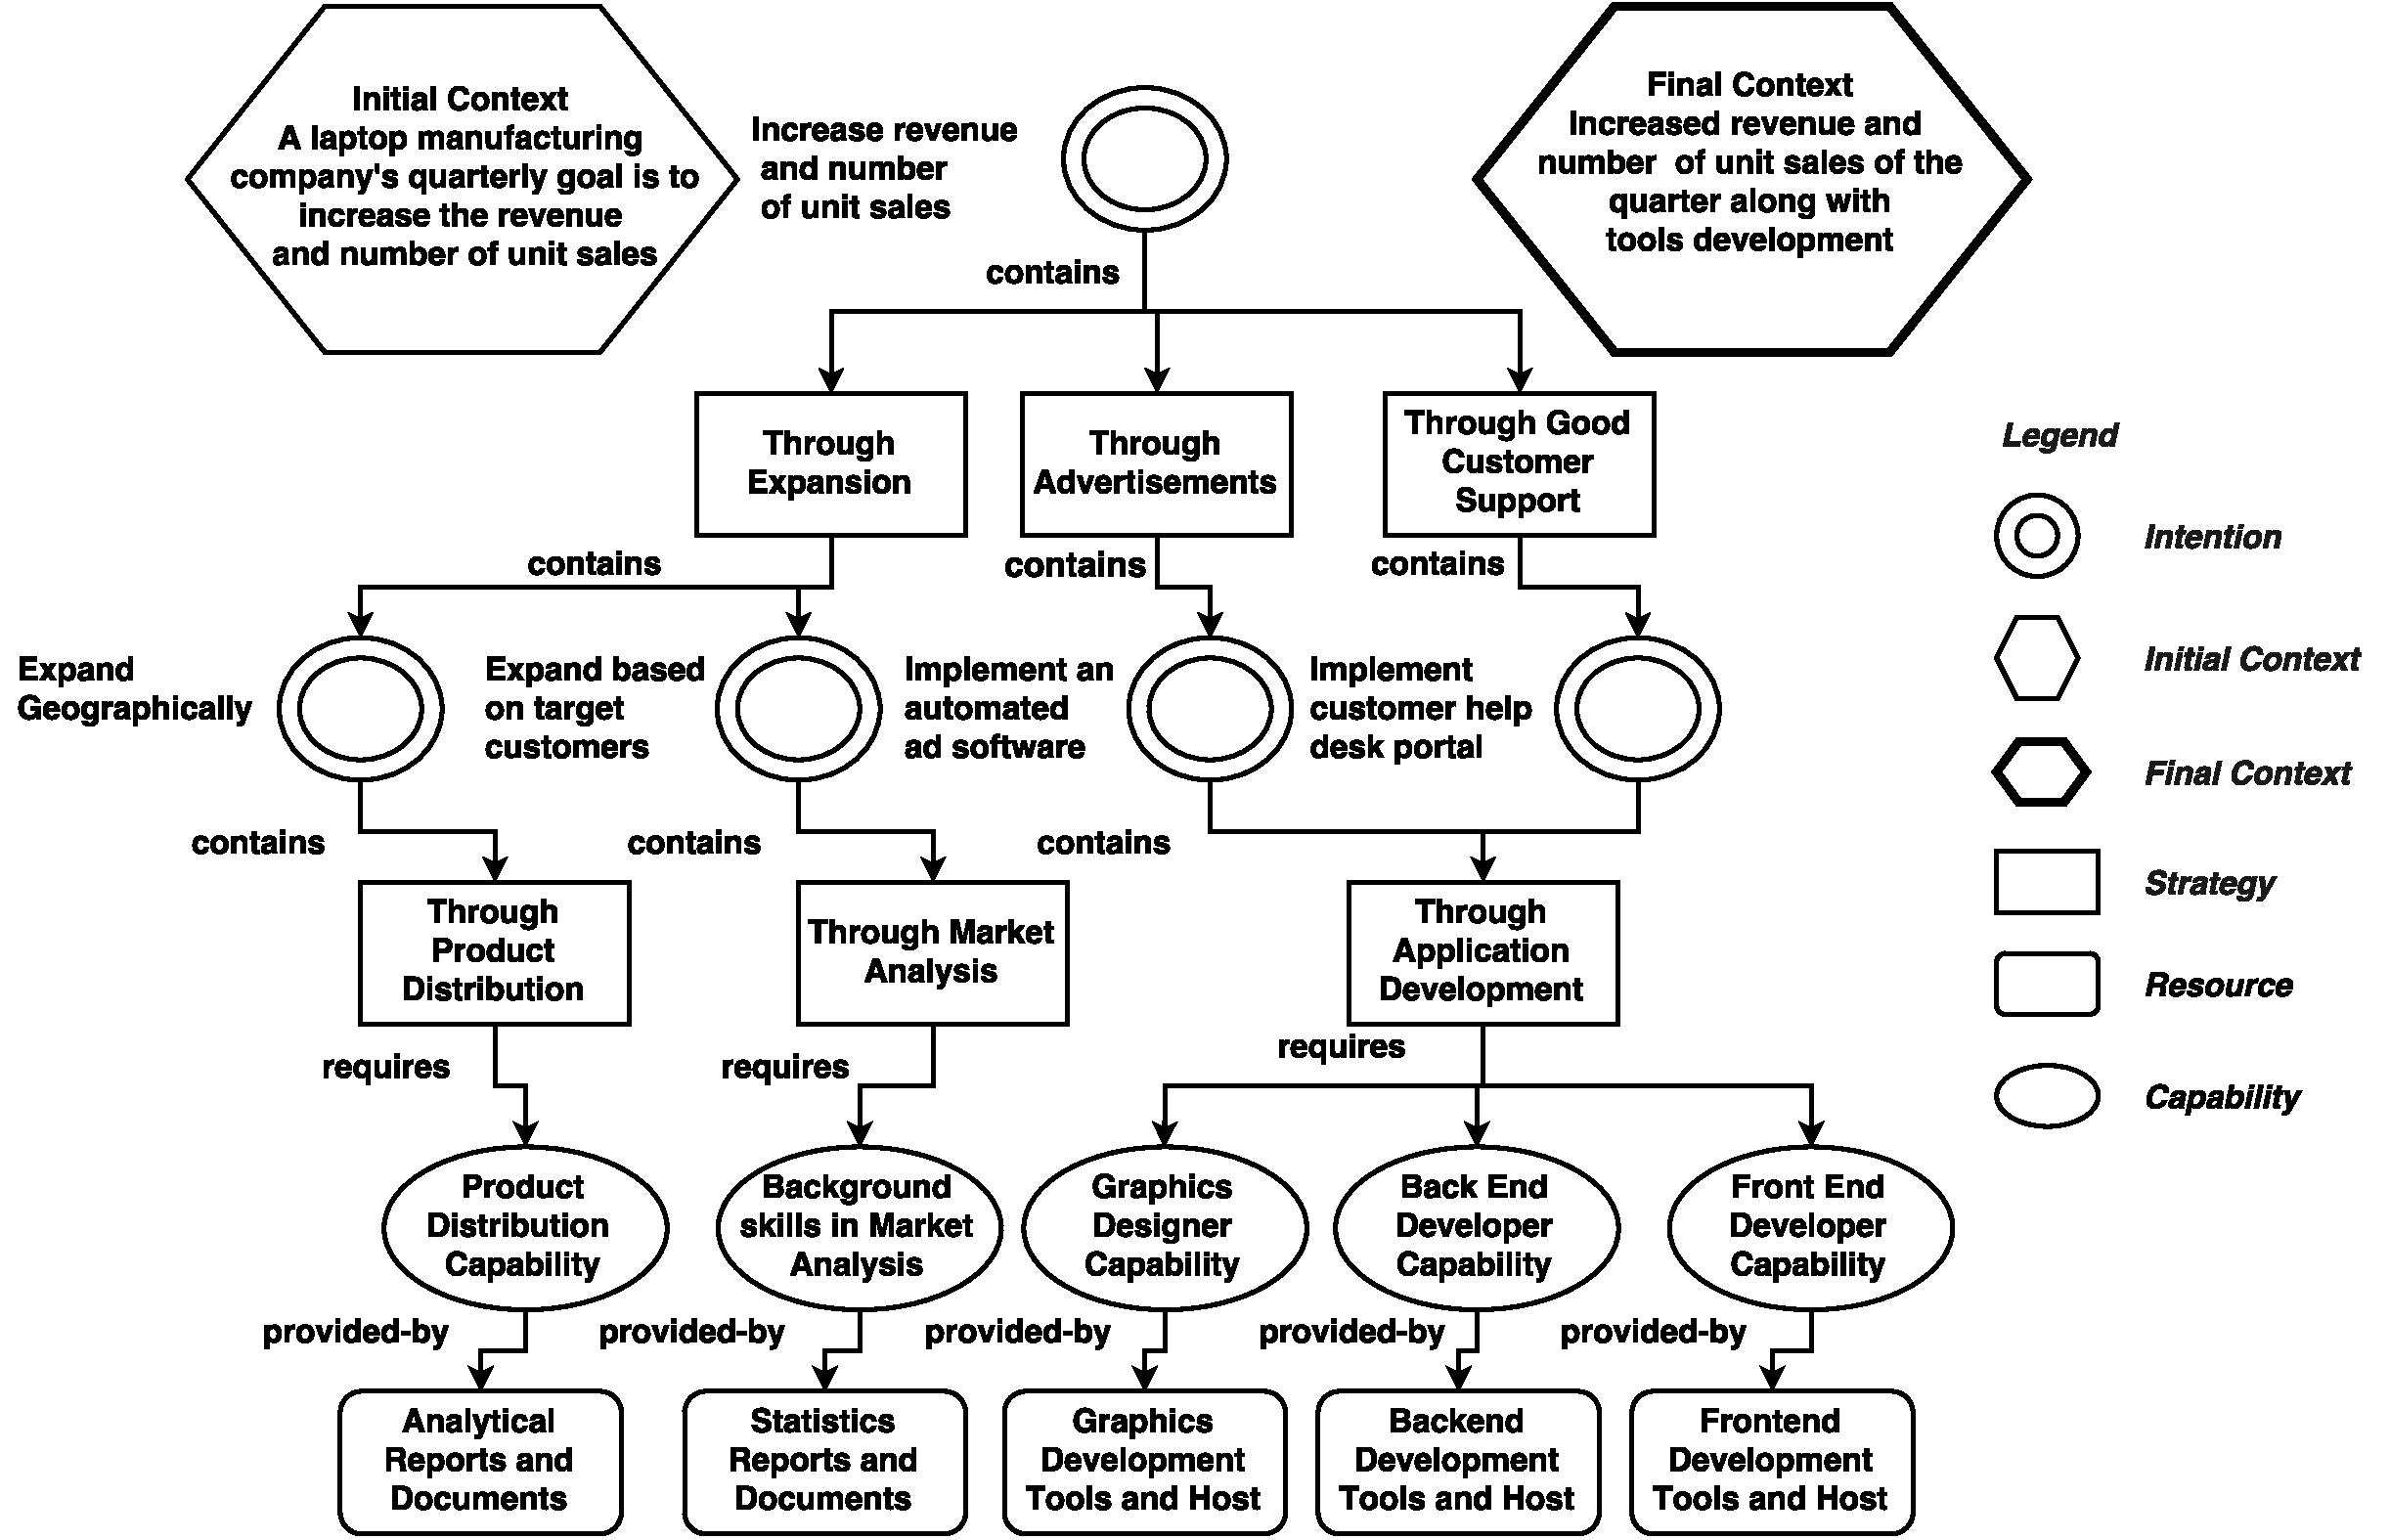
\includegraphics[width=\textwidth]{MotivatingScenario.pdf}
 	\caption{Motivating Scenario}
 	\label{fig:motivatingscenario}
 \end{figure}

 The Strategy view  in the Figure\ref{fig:motivatingscenario} depicts big picture of each strategy. Strategies are associated with both intentions and capabilities. Capabilities are related to resources. As each intention needs certain capability to successfully execute the intention they both are connected using the verb \textit{"requires"}. Resources are the potential holder of the capability i.e., to satisfy a capability we need resources. The capability and its associated resources are linked using the verb \textit{"satisfied-by"}. 






%%%%%%%%%%%%%%%%%%%%%%%%%%%%%%%%%%%%%%%%%%%%%%%%%%%%%%%%%%%%%%%%%%%%%%%%%
\section{An Abstract View of Entity Types}
\label{sec:entities}
%%%%%%%%%%%%%%%%%%%%%%%%%%%%%%%%%%%%%%%%%%%%%%%%%%%%%%%%%%%%%%%%%%%%%%%%%
 --- This section discusses in details, about each entity types of the motivating scenario and 
 their images---
 

%%%%%%%%%%%%%%%%%%%%%%%%%%%%%%%%%%%%%%%%%%%%%%%%%%%%%%%%%%%%%%%%%%%%%%%%%
\subsection{Organizational Intentions} 
\label{sec:intentions}
%%%%%%%%%%%%%%%%%%%%%%%%%%%%%%%%%%%%%%%%%%%%%%%%%%%%%%%%%%%%%%%%%%%%%%%%%
Intentions can contradict themselves, for example in our motivating scenario IT system managers are not willing to give up the systems they are working for a long time even if it is a better solution for organization as whole . This real life example scenario has been provided in the thesis work \cite{Sierr2015} and also it has been suggested that such contradicting intentions has to be handled in some way. Thus our developed web editor has also provision to add both sub-intentions and contradicting intentions for any intention.  


%%%%%%%%%%%%%%%%%%%%%%%%%%%%%%%%%%%%%%%%%%%%%%%%%%%%%%%%%%%%%%%%%%%%%%%%%
\subsection{Organizational Strategies} 
\label{sec:strategies}
%%%%%%%%%%%%%%%%%%%%%%%%%%%%%%%%%%%%%%%%%%%%%%%%%%%%%%%%%%%%%%%%%%%%%%%%%
Strategies are used to identify the most appropriate method of utilizing the capabilities. 


%%%%%%%%%%%%%%%%%%%%%%%%%%%%%%%%%%%%%%%%%%%%%%%%%%%%%%%%%%%%%%%%%%%%%%%%%
\subsection{Organizational Capabilities}
\label{sec:capabilities}
%%%%%%%%%%%%%%%%%%%%%%%%%%%%%%%%%%%%%%%%%%%%%%%%%%%%%%%%%%%%%%%%%%%%%%%%%
Describing  capabilities as \textit{ability to do something}, suggests that capabilities are related to intentions. Resources tends to posses certain capabilities that allow them to do something that they want or need to do something. 



%%%%%%%%%%%%%%%%%%%%%%%%%%%%%%%%%%%%%%%%%%%%%%%%%%%%%%%%%%%%%%%%%%%%%%%%%
\subsection{Organizational Resources} 
\label{sec:resources}
%%%%%%%%%%%%%%%%%%%%%%%%%%%%%%%%%%%%%%%%%%%%%%%%%%%%%%%%%%%%%%%%%%%%%%%%%

Each resources has different types of relationship with other resources based on how they communicate with other resources \cite{Sungur2015}. For example in our motivating scenario described in Section \ref{sec:scenario} has one of the sub-intention as \textit{through excellence}. This sub-intention can be achieved by providing skills improvement training to the employees or by recuriting newly skilled employee. Here the manager has permissions to decide whether to improve skills of existing employee or recruit new employee. But the team lead has restricted permission like what type of skills are required for the project based on decision of manager. The Informal Process Essentials (IPE) approach proposed by Sungur et al. \cite{Sungur2015}, paves the way to create models with definitions of key actors e.g manager, team lead and definitions of suppoting resources such as Mediawiki \footnote{http://www.mediawiki.org/}.

A \textit{resource organizer} is responsible for gathering definitions about the resources which are required by business experts for modeling \cite{Sungur2014a}.  



%%%%%%%%%%%%%%%%%%%%%%%%%%%%%%%%%%%%%%%%%%%%%%%%%%%%%%%%%%%%%%%%%%%%%%%%%
\subsection{Organizational Processes} 
\label{sec:processes}
%%%%%%%%%%%%%%%%%%%%%%%%%%%%%%%%%%%%%%%%%%%%%%%%%%%%%%%%%%%%%%%%%%%%%%%%%

%%%%%%%%%%%%%%%%%%%%%%%%%%%%%%%%%%%%%%%%%%%%%%%%%%%%%%%%%%%%%%%%%%%%%%%%%
\subsection{Informal Process Instances} 
\label{sec:ipinstances}
%%%%%%%%%%%%%%%%%%%%%%%%%%%%%%%%%%%%%%%%%%%%%%%%%%%%%%%%%%%%%%%%%%%%%%%%%
\cleardoublepage
\chapter{Requirements for Supporting Intention-oriented Organizational Modeling}
\label{chap:analysis}
This chapter positions the thesis work in the field of organizational modeling with respect to the other existing approaches. The first section provides detailed requirement analysis of intention-oriented organizational modeling. The final section provides a detailed literature review about the existing approaches. A detailed evaluation of the existing approaches with the proposed requirements is also provided in the last section.

%%%%%%%%%%%%%%%%%%%%%%%%%%%%%%%%%%%%%%%%%%%%%%%%%%%%%%%%%%%%%%%%%%%%%%%%%
\section{Requirement Analysis of Intention-oriented Organizational Modeling}
\label{sec:requirementssupoorting}
%%%%%%%%%%%%%%%%%%%%%%%%%%%%%%%%%%%%%%%%%%%%%%%%%%%%%%%%%%%%%%%%%%%%%%%%%
The requirements of intention-oriented organizational modeling has been derived from existing literatures \cite{McManus2007, Mandic2010 ,Bleistein2006, Lacom, Brambilla2012} and from the motivating scenario described in Chapter \ref{chap:motivatingScenario}. 

\subsection{Organizational Intention Transparency (R1)}
An intention can be broken down into definitive actionable components upon which individual resources can act. When these lower level intentions are made achievable for individual resources, they can be combined to provide successful execution of higher level intention. This requires privilege for different organizational members to observe lower level and higher level intentions. Additionally, intentions should also be traceable in the different levels of the organizational hierarchy. This means that the status of each intention can be accessed by members in different levels of the organizations based on their privilege. This level of transparency within an organization reduces inefficiencies in intention execution, and is a key factor in attracting and retaining high performers in the labor market \cite{McManus2007}. Requirement R1 has to be satisfied in the modeling phase itself as the designing of intentions, strategies and their recursive structures are done during the modeling phase. The main pre-requisites for this requirement to be satisfied are intentions can be refinable and organizational members can view intentions at different levels. 

\subsection{Organizational Strategy-based Cost Estimation (R2)}
Linking strategies with capabilities that has matching resource enable us a cost estimation for each strategy. This is because strategies are associated with organizational capabilities which in turn is associated with organizational resources. To incorporate the cost estimation of strategies, we have to understand the recursive structure of the strategies associated with process definitions and then with the resource definitions. Further on, the cost of a strategy can be analyzed using the costs of derived process definitions and then with resource definitions. Including resources cost in strategy cost calculation is important. This is achieved by associating resource models' cost with process models' cost. The recursion is stopped when each resource definition is associated with cost. At the moment an intention is achieved, some resources should be allocated to maintain the desired state \cite{Mandic2010}. Since intentions are achieved through strategy we should also be able to calculate cost of intention based on cost of its strategies. Allocation of resources is mainly done at the operational level, hence requirement R2 has to be satisfied during the modeling phase. It is essential to do cost calculation during modeling phase as it helps to determine the affordable resources. The pre-requisites to satisfy this requirement are resources associated with cost and strategy cost estimation that includes all recursive structure.

\subsection{Organizational Strategy Achieve-ability Estimation (R3)}
 The validity of an organizational strategy is assured when the strategy is associated with valid capbilities. A capability can be considered as a valid capability when it has matching resource. A valid strategy can be implemented as independent informal process. Lower-level entities can be validated against higher-level entities, thus enabling validation of strategic alignment of strategies' recursive structure \cite{Bleistein2006}. Requirement R3  can be done during the modeling phase of the process as strategy achieve-ability estimations are done before starting the execution of the process. For a strategy to be achieve-able the required pre-requisites are, strategy should have associated with valid capability that is associated with matching resources and the strategy can be implemented as independent informal process.
 
\subsection{Intention Oriented Working Style (R4)}
As each member of the organization is aware of the higher level and lower level intentions, member can engage for explicit intentions. Intention orientation is the degree to which a person or organization focuses on tasks and its end results. Strong intention orientation advocates that focus on a task is more. Such a focused task ends in a result that is favorable to both employees and organization. Those with strong intention orientation will be able to accurately judge the effects of reaching the intention as well as the ability to fulfill that particular intention with current resources and skills \cite{Lacom}. Hence we associate processes implicitly with intentions through strategies which enables people to work towards certain intentions. The distinction between explicit knowledge of each low level intention should not be seen as a division but rather as a continuum which aligns towards achieving the higher level intention. Though requirement R4 seems to be part of requirement R1, R4 happens during modeling phase and could also happen during execution phase due to the dynamic nature of informal process. The pre-requisites for this requirement are satisfaction of R1 and organizational members requiring understanding of the intentions.  

\subsection{Participative Organizational Modeling (R5)}
 Different members of an organization participate to create organizational intentions, as a result organizational models are shaped based on input proided by different members but directed by the executives. The social extension of a business process can be regarded as a process optimization phase, where the organization seeks efficiency by extending the reach of a business process to a broader class of people \cite{Brambilla2012}. Since the requirement itself is about developing models based on input from different organizational members, the requirement has to be satisfied during modeling phase. The pre-requisites to satisfy this requirement are satisfaction of R1 and intention-oriented modeling has to be done based on input provided by different members of the organization.  
 
 The requirement satisfaction phase and pre-requisites to satisfy each requirement is provided in the Table \ref{tab:subrequirements}

\begin{table} [htbp]
	\centering
	\begin{tabular} {p{2.5cm}p{3cm}p{8cm}}
		\toprule
		\textbf{Requirement} & \textbf{Requirement Satisfaction Phase} & \textbf{Pre-requisites}    \\
		\midrule                                                                                                               
		R1    & Modeling phase    &(1) Main intention can be refinable, (2) Organizational members can view the intentions at different levels    \\ 
		
		R2   & Modeling phase    &(1) Resources associated with cost, (2) Strategy cost estimation that includes all recursive structure \\         
			
		R3   & Modeling phase       &(1) A valid capability which has matching resource, (2) Strategies can be implemented as independent informal process \\      
		
		R4   & Modeling and Execution phases     &(1) Satisfaction of R1, (2) Organizational members require understanding of the intentions and how they can be reached \\                         
			
		R5  &Modeling phase  &(1) Satisfaction of R1, (2) Intentions has to be modeled based on the input provided by different members of the organization               \\ 
		    
		\bottomrule
	\end{tabular}
	\caption{Requirements Analysis}
	\label{tab:subrequirements}
\end{table}

%%%%%%%%%%%%%%%%%%%%%%%%%%%%%%%%%%%%%%%%%%%%%%%%%%%%%%%%%%%%%%%%%%%%%%%%%
\section{Literature Review and Evaluation of Related Work}
\label{sec:literaturereview}
%%%%%%%%%%%%%%%%%%%%%%%%%%%%%%%%%%%%%%%%%%%%%%%%%%%%%%%%%%%%%%%%%%%%%%%%%
In the literature, several work has been done in order to support and automate the business process modeling such as strategy-driven \cite{Bider2005}, activity-centric\cite{Yarosh2009}, activity-oriented \cite{Leymann2000}, artifact-centric \cite{Cohn2009}, capability-driven \cite{Stirna2012}, ArchiMate \cite{Group2012} and subject-oriented \cite{Fleischmann2013}.  A detailed description about these approaches and their level of satisfying the requirements mentioned in Section \ref{sec:requirementssupoorting} has also been provided. 

\subsection{Strategy-driven} 
Strategy driven approach is decision oriented modeling approach that focus on goals of the processes and refine goals until the operational level. This approach defines business process in terms of goals and strategies in order to achieve the goals. It also uses map representation system that contains goals and strategies. In this approach, goals are refinable and details regarding visibility of goals has not been addressed. Thus requirement R1 is partially satisfied as the approach satisfies one of the pre-requisites. The details about cost of strategy and resources is not addressed. Hence requirement R2 is not satisfied. The requirement R3 contradicts with the process rule of this approach which states that "There is no goal/strategy in the map that can be considered as the subset of another one". So achieve-ability estimation of a strategy based on its association with valid capability cannot be determined in this approach. Requirement R4 is partially satisfied, as it satisfies R1 partially and this approach also requires understanding of goals by the organizational members. The requirement R5 is partially satisfied, as the approach partially satisfies requirement R1. But another pre-requisite (i.e., intentions has to be modeled based on the inputs provided by different members of the organization) to satisfy R5, is not addressed by the approach. 

\subsection{Activity-oriented} 
Traditional workflows are based on activity-oriented process models and executed based on these models. Requirements R1, R4 and R5 are not satisfied as details of intentions and modeling based on intentions are not provided. The details about cost calculation is addressed but cost calculation of strategies are not addressed. Hence, requirement R2 is partially satisfied. Though this approach does not support sub-processes directly, it provides support for plugging in sub process extensions which can be executed as independent process. Since none of the pre-requisites of requirement R3 is met, the requirement is not satisfied by the approach. 

\subsection{Activity-centric} 
The activity-centric approach also supports knowledge workers by providing shared activity constructs (i.e., activity-oriented constructs) as a computational unit for organizing the work. Though this approach provides team level view of past and ongoing work by supporting propagation of completed activities to the existing activities, the approach is not goal-oriented. Thus requirements R1, R4 and R5 are not met. The information about cost of achieving a goal or activity has not been mentioned. Thus requirement R2 is not satisfied. The approach also does not provide any information regarding association of strategies with valid capability.  
 
\subsection{Artifact-centric} 
Artifact-centric is a data-centric approach to model business processes based on business relevant data. The artifact-centric approach combines business data (artifacts) and business process in a holistic way. Requirements R1, R4 and R5 are not satisfied as details of intentions and modeling based on intentions are not provided. The requirement R2 which is about cost calculation is also not addressed. Though the approach allows modularity of business operations at various levels, it is not associated with strategies. Hence requirement R3 is also not satisfied. 

\subsection{Capability-driven} 
The capability driven approach also proposes to support the changing environment of organizations. This approach aims to aid development of business models by connecting goals and capabilities. Though goals are refinable in this approach, there is no information about the visibility of goals. Hence requirement R1 is partially met. This approach claims that, it overcomes the challenge of high cost in developing applications but there is no clear details about how cost calculation is done, hence requirement R2 is not addressed. It does not provide any information about strategy associated with valid capability. Hence, requirement R3 is also not addressed. The first pre-requisite for requirement R4 is partially satisfied and second pre-requisite is also satisfied by the approach. Thus, requirement R4 is partially satisfied. The first pre-requisite for requirement R5 is partially satisfied and second pre-requisite is not addressed by the approach. Thus, requirement R5 is also partially satisfied. 

\subsection{ArchiMate}
ArchiMate provides an integrated modeling approach by allowing to model based on both activities, i.e., business process and business functions such as knowledge, resources, etc. ArchiMate allows modeling based on goals and provides visibility of whole process, supports viewpoints in different levels of modeling. Thus requirement R1 is addressed. Requirement R2 which is cost calculation of goals is addressed. Thus requirement R2 is partially satisfied as details regarding the cost calculation of strategies not provided. The pre-requisites to satisfy requirement R3 are not addressed. Thus, requirement R3 is not addressed. Requirement R4 is satisfied because both the first and second pre-requisites are satisfied. Similarly, requirement R5 is also satisfied because the approach also satisfies first and second pre-requisites.  

\subsection {Summary of the Evaluation}
 The approach \textit{Adaptive Case Management}, proposed by Hermann et. al \cite{Herrmann2011} bridges the gap between business processes management and flexibility in adapting knowledge intensive processes by defining activities and re-using created activity structure. When the required activities changes dynamically, capturing them for re-use are not helpful \cite{Sungur2015}. Though the approach \textit{Ad-hoc and Collaborative Processes} proposed by Dustdar et. al. overcomes the challenges in process aware collaborations, defining activities in ad-hoc fashion does not support human actor in various cases \cite{Sungur2015}. The Table \ref{tab:evaluationoftheapproach}, shows the evaluation of related works based on the derived requirements. 

\begin{table}[]
	\scriptsize 
	\centering
	\begin{tabular}{p{2cm}p{2.5cm}p{2.5cm}p{2.5cm}p{2.5cm}p{2.5cm}}
	\toprule
		Approach & R1               & R2               & R3         & R4       & R5        \\
	\midrule
	Strategy-driven & (1)+Refinable, (2)-Not Addressed  & (1)-Not Addressed, (2)-Not Addressed  & (1)-Not Addressed, (2)-Not Addressed  & (1)~R1 partially satisfied, (2)+Addressed  & (1)~R1 partially satisfied, (2)-Not Addressed \\
	Activity-oriented & (1)-Activity-oriented, (2)-Activity-oriented
	 &(1)~Addressed, (2)- Not Addressed  & (1)-Not addressed, (2)-Not addressed   &(1)-Activity-oriented, (2)-Activity-oriented  &(1)-Activity-oriented, (2)-Activity-oriented \\
	Activity-centric & (1)-Activity-centric, (2)-Activity-centric  & (1)-Not Addressed, (2)-Not Addressed  & (1)-Not Addressed, (2)-Not Addressed  &  (1)-Activity-centric, (2)-Activity-centric &  (1)-Activity-centric, (2)-Activity-centric \\
	Artifact-centric    & (1)-Artifact-centric, (2)-Artifact-centric  & (1)-Not Addressed, (2)-Not Addressed  & (1)-Not Addressed, (2)-Not Addressed  & (1)-Artifact-centric, (2)-Artifact-centric & (1)-Artifact-centric, (2)-Artifact-centric  \\ 
	Capability-driven   & (1)+Refinable, (2)-Not addressed & (1)-Not addressed, (2)-Not addressed   & (1)-Not addressed, (2)-Not addressed  & (1)~R1 partially satisfied, (2)+Addressed  & (1)~R1 partially satisfied, (2)-Not Addressed  \\
	ArchiMate  & (1)~Addressed, (2)- Not Addressed & (1)+Addressed, (2)+Addressed & (1)-Not addressed, (2)-Not addressed  & (1)+R1 satisfied, (2)+Addressed & (1)+R1 satisfied, (2)+Addressed\\
	\bottomrule   
	\end{tabular}
	\caption{Summary of the Evaluation}
	\label{tab:evaluationoftheapproach}  
\end{table}


From the Table \ref{tab:evaluationoftheapproach}, one could comprehend that none of the evaluated approaches satisfy all the requirements together. Thus, we propose a new intention-oriented organizational modeling approach in Chapter \ref{chap:approach} that satisfies all of the requirements. 
 



\cleardoublepage
\chapter{An Approach to Resource-centric Organizational Modeling}
\label{chap:approach}

%%Description of the approach you have taken to solve the scientific or technical problem which you were posed.
%%Outline the design, the methodology and overall structure of your experinmental approach.

%%%%%%%%%%%%%%%%%%%%%%%%%%%%%%%%%%%%%%%%%%%%%%%%%%%%%%%%%%%%%%%%%%%%%%%%%
\section{Overview of Modeling Process}
\label{sec:overviewmodelingprocess}
%%%%%%%%%%%%%%%%%%%%%%%%%%%%%%%%%%%%%%%%%%%%%%%%%%%%%%%%%%%%%%%%%%%%%%%%%
 The Organizational Modeling element notation has been selected as per the guidelines mentioned in the paper by Moody \cite{Moody2009}. Also by observing  the fact that business process modelers are already well-known with the present process modeling notations such as Business Process Modeling Notation 2.0 (BPMN) \cite{bpm2011} and ArchiMate notation \cite{arc2013}, the shape depiction of organizational model elements are designed similar to those existing process notations. 




%%%%%%%%%%%%%%%%%%%%%%%%%%%%%%%%%%%%%%%%%%%%%%%%%%%%%%%%%%%%%%%%%%%%%%%%%
\section{Evaluation of the Approach}
\label{sec:evaluationoftheapproach}
%%%%%%%%%%%%%%%%%%%%%%%%%%%%%%%%%%%%%%%%%%%%%%%%%%%%%%%%%%%%%%%%%%%%%%%%%

The Table \ref{tab:evaluationoftheapproach}, provides an evaluation of the approaches. The description of each symbol used in the  Table \ref{tab:evaluationoftheapproach} is given as a legend.


\begin{center}
	\begin{longtable}{p{5cm}p{2cm}p{2cm}p{2cm}p{2cm}p{2cm}} 
		\toprule 
		\textbf{Approach} & \textbf{RO1}  & \textbf{RO2}  & \textbf{RO2}  & \textbf{RO4}  & \textbf{RO5} \\
		\midrule
		\endfirsthead
		\\
	   	Strategy-Driven & -  & -  & +  & -  & + \\
	   	Activity-centric System  \\
	   	Activity-oriented System  \\
	   	Artifact-centric System  \\
	   	Capability-driven Development \\
	   	ArchiMate \\
	    Subject-Oriented System \\
		
		\bottomrule
		\caption{Evaluation of the Approach}
		\label{tab:evaluationoftheapproach}
	\end{longtable}	
\end{center}

Legend :
\begin{description}
	\item[+]  Addressed in the approach
	\item[-]  Not addressed in the approach
	\item[\~] Partially addressed in the approach
\end{description}

%%%%%%%%%%%%%%%%%%%%%%%%%%%%%%%%%%%%%%%%%%%%%%%%%%%%%%%%%%%%%%%%%%%%%%%%%
\section{Specifications}
\label{subsec:specifications}
%%%%%%%%%%%%%%%%%%%%%%%%%%%%%%%%%%%%%%%%%%%%%%%%%%%%%%%%%%%%%%%%%%%%%%%%%
In order to realize the web editor of Intention-centric Organizational Modeling, a formal inquiry has been done and concluded with the below specifications.

\begin{enumerate}   
	\item \textbf{Clojurescript} as the programming language
	\item \textbf{IntelliJIDEA} as the IDE
	\item \textbf{MVC} as the architecture pattern
	\item \textbf{Re-frame} as the pattern for writing SPAs in ClojureScript, using Reagent	
\end{enumerate}

%%%%%%%%%%%%%%%%%%%%%%%%%%%%%%%%%%%%%%%%%%%%%%%%%%%%%%%%%%%%%%%%%%%%%%%%%
\section{Architecture}
\label{subsec:mvcarch}
%%%%%%%%%%%%%%%%%%%%%%%%%%%%%%%%%%%%%%%%%%%%%%%%%%%%%%%%%%%%%%%%%%%%%%%%%
 The architecture of the UI editor is based on the \textbf{Model-View-Control (MVC)} design pattern. The MVC paradigm allows to separate business logic from the code that controls presentation and event handling \cite{Oracle2016}.Each entity view in the web page is made up of combination of at least on Model and View, and one or more Controls. The individual files which acts an Model, View and Controller has been shown in the Figure \ref{fig:mvc_arch}

\begin{itemize}
	\item \textbf{Model} artifact stores the required data structure for web-editor. In the developed model artifact, the four main types of data stored inside the artifact are intentions, strategies, capabilities and informal process instances. 
	\item \textbf{View} artifact contains HTML elements and HTML constructs that describe the way of displaying the data from Model to the user.
	\item \textbf{Control} artifact contains the handler functions which can only change the model. Even the initial values of the model are put inside the control. 
\end{itemize}


\begin{figure}
	\centering
	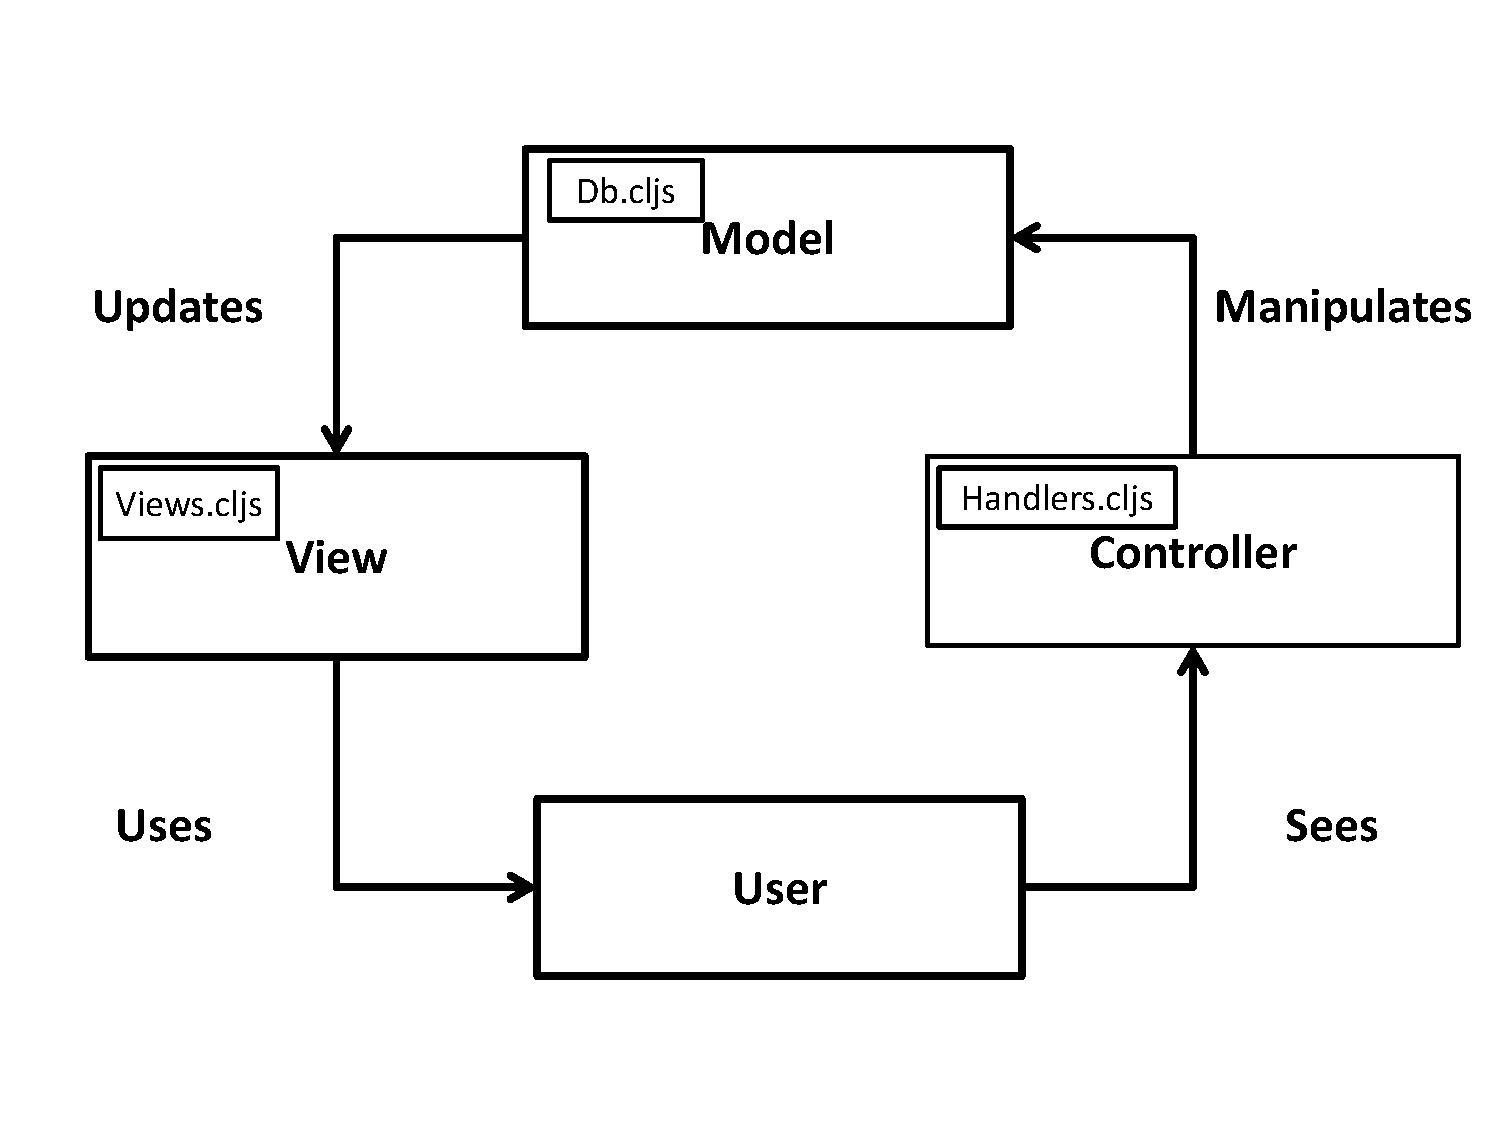
\includegraphics [width= 0.75\textwidth]{mvc_arch.pdf}
	\caption{Relationship between developed web editor artifacts and MVC architecture components}
	\label{fig:mvc_arch}
\end{figure}


%%%%%%%%%%%%%%%%%%%%%%%%%%%%%%%%%%%%%%%%%%%%%%%%%%%%%%%%%%%%%%%%%%%%%%%%%
\subsubsection{Example: Component using MVC Pattern }
%%%%%%%%%%%%%%%%%%%%%%%%%%%%%%%%%%%%%%%%%%%%%%%%%%%%%%%%%%%%%%%%%%%%%%%%%
 The Figure \ref{fig:mvc_arch} below shows the simplifed version of how the components interact with each other using the Model-View-Control (MVC) pattern, for the functionality adding new entity data. This functionality is same for all the types intentions, strategies, capabilities and informal proceess instances and below is the detailed explanation of each interaction.

\begin{enumerate}
	\item User clicks the tab \textbf{Add New} in the web editor.
	\item View, in response to the user click displays the UI component for entering the new entity data details.
	\item User enters the required basic details for adding new entity data and clicks save button.
	\item View dispatches the data to Control, which can only modify the Model.
	\item Control inserts/updates data into the model.
	\item View displays the updated model as it has been subscribed to the model.
\end{enumerate}

\begin{figure}
	\centering
	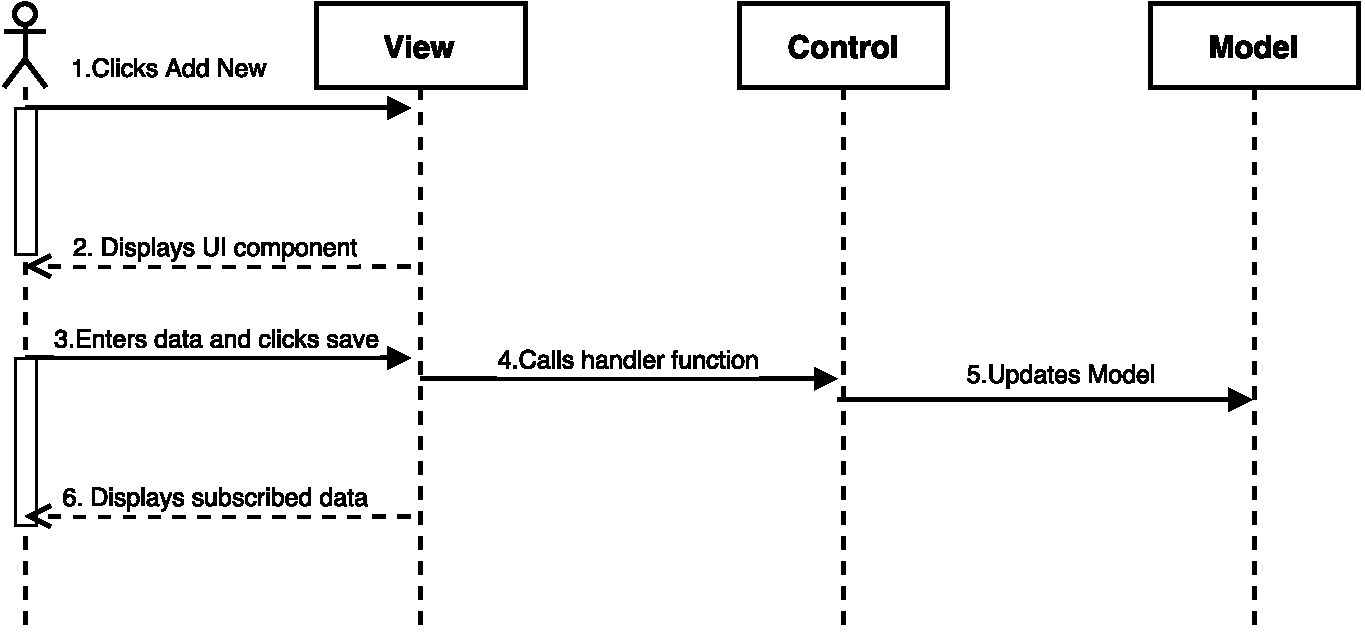
\includegraphics [width= \textwidth]{mvc_pattern.pdf}
	\caption{MVC Pattern of adding new entity}
	\label{fig:mvc_pattern}
\end{figure}


%%%%%%%%%%%%%%%%%%%%%%%%%%%%%%%%%%%%%%%%%%%%%%%%%%%%%%%%%%%%%%%%%%%%%%%%%
\subsection{Using Reagent Framework}
\label{subsec:reagent}
%%%%%%%%%%%%%%%%%%%%%%%%%%%%%%%%%%%%%%%%%%%%%%%%%%%%%%%%%%%%%%%%%%%%%%%%%

The Reagent Framework architecture has been reused Fig. \ref{fig:mvc_pattern23} \footnote{Source: https://github.com/Day8/re-frame}


\begin{figure}
	\centering
	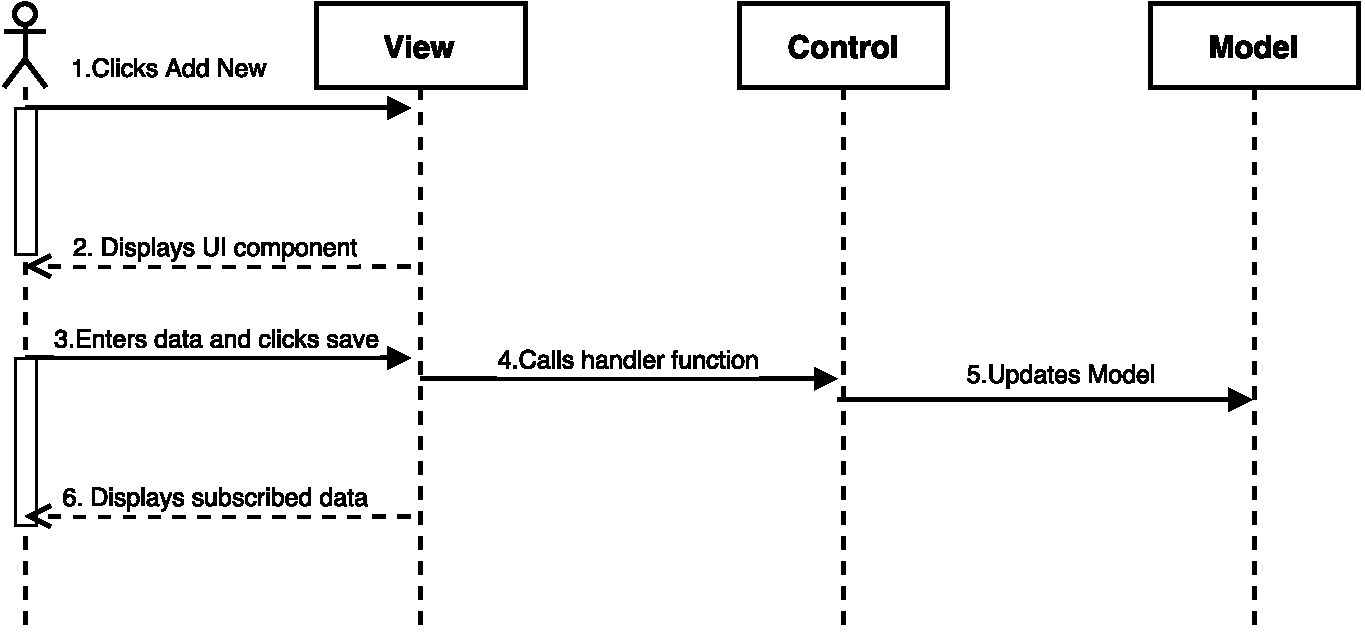
\includegraphics [width= \textwidth]{mvc_pattern.pdf}
	\caption{MVC Pattern of adding new entity }
	\label{fig:mvc_pattern23}
\end{figure}



%%%%%%%%%%%%%%%%%%%%%%%%%%%%%%%%%%%%%%%%%%%%%%%%%%%%%%%%%%%%%%%%%%%%%%%%%
\section{Entity Type Relationship}
\label{sec:enttyperelation}
%%%%%%%%%%%%%%%%%%%%%%%%%%%%%%%%%%%%%%%%%%%%%%%%%%%%%%%%%%%%%%%%%%%%%%%%%

%%%%%%%%%%%%%%%%%%%%%%%%%%%%%%%%%%%%%%%%%%%%%%%%%%%%%%%%%%%%%%%%%%%%%%%%%
\subsection{Context Intention Relationship}
\label{sec:ctxintrel}
%%%%%%%%%%%%%%%%%%%%%%%%%%%%%%%%%%%%%%%%%%%%%%%%%%%%%%%%%%%%%%%%%%%%%%%%%
Intentions connect initial context definitions with final context definitions. \ref{fig:CtxIntRel}


\begin{figure}
	\centering
	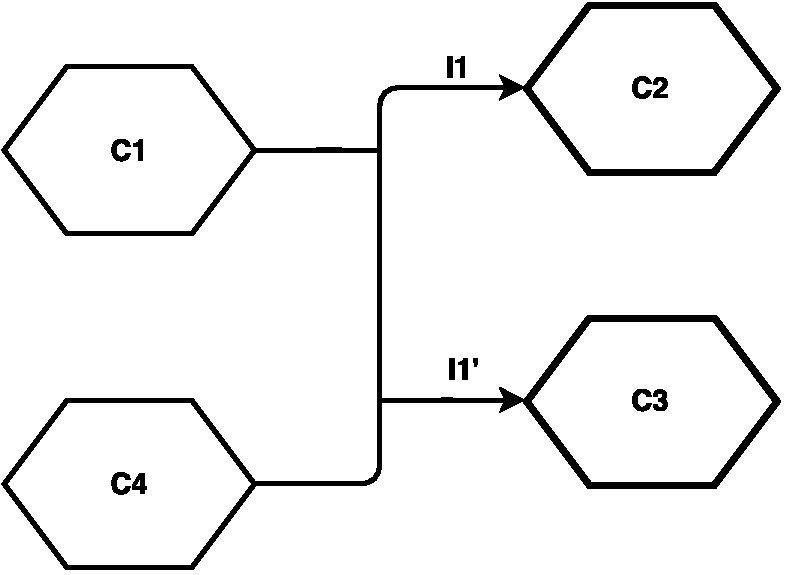
\includegraphics [width= 0.5\textwidth]{CtxIntRel.pdf}
	\caption{Context Intentions Relationship}
	\label{fig:CtxIntRel}
\end{figure}


%%%%%%%%%%%%%%%%%%%%%%%%%%%%%%%%%%%%%%%%%%%%%%%%%%%%%%%%%%%%%%%%%%%%%%%%%
\section{User Interface Diagram}
\label{sec:uidiagram}
%%%%%%%%%%%%%%%%%%%%%%%%%%%%%%%%%%%%%%%%%%%%%%%%%%%%%%%%%%%%%%%%%%%%%%%%%

%%%%%%%%%%%%%%%%%%%%%%%%%%%%%%%%%%%%%%%%%%%%%%%%%%%%%%%%%%%%%%%%%%%%%%%%%
\section{Design Methodology}
\label{sec:designmethodology}
%%%%%%%%%%%%%%%%%%%%%%%%%%%%%%%%%%%%%%%%%%%%%%%%%%%%%%%%%%%%%%%%%%%%%%%%%

On the left list we should have all organizational context definitions and on the right one only ones that are contained in an informal process. The dropdown box of the initial and final context defines the selection inside of an informal process, thus right side.

So, in db.cljs, we should have only a list of context definitions no :initial-contexts and :desired-final-contexts. Only :organizational-contexts and under this all available contexts. Under the left list, we present these elements. Right list should refer to the initial-context, final-contexts, etc. of the informal process model depending on the selection of the dropbox button. For instance if we have initial contexts selected on the dropdown box, we should present the initial contexts in the right list.

I have changed the code accordingly and provided you an example how you should change data from views.cljs. All data should be stored in db.cljs. This applies to the text fields of all elements. Whenever, we want to update something we need to update the map in db.cljs and this will be propagated to the views.


On the left side of each list item, you should present all available items of context definitions or intentions whatever type is selected there. On the right side only the ones contained in the respective informal process model. Inside of another entity, you should refer to other entities using their ids and these ids should be resolved using, for instance, intentions vector. You check each intention in the intentions vector, if it’s id is the same as the id you are looking for it, you found it and you use the information about it.  


Please align it with the structure and names of the IPSM.xsd. Each variableName like this is written like variable-name. Each complex type is a map each attribute is a key value pair and each element in another element is another key value pair.

\begin{Listing}
	\begin{lstlisting}
	:entity-data {:informal-process-definitions [ipd1 ipd2]
	:context-definitions [ctx1 ctx2 ctx3]
	:intentions [int1 int2]} 
	\end{lstlisting}
	\caption{Entity data definition inside db.cljs}
	\label{lst:entitydatalist}
\end{Listing}





\cleardoublepage
\chapter{Case Study on a Manufacturing Company}
\label{chap:casestudy}

In this chapter, the first three sections provide the implementation details along with the reason for making certain decisions regarding the implementation of web-based modeling tool. The fourth section provides an architecture of the functioning system and fifth section provides application flow of the functioning system. The sixth section explains how motivating scenario has been realized using the proposed modeling approach. Successful modeling of the motivating scenario using the developed editor serves as a proof for usability of the web-based modeling tool. Hence, the final section validates the system by evaluating it with the requirements for supporting intention-oriented organizational modeling. 

%%%%%%%%%%%%%%%%%%%%%%%%%%%%%%%%%%%%%%%%%%%%%%%%%%%%%%%%%%%%%%%%%%%%%%%%%
\section{Technologies and Frameworks}
\label{subsec:specifications}
%%%%%%%%%%%%%%%%%%%%%%%%%%%%%%%%%%%%%%%%%%%%%%%%%%%%%%%%%%%%%%%%%%%%%%%%%
In order to, realize the approach presented in the Section \ref{sec:topdownapproach} of the previous Chapter \ref{chap:approach}, a formal inquiry was done to choose suitable technologies and frameworks required. The below specifications were finalized and \textit{single page web application} (SPA) using\textit{client-side scripting} was chosen. The single page web application is a web application that fits on a single web page with user experience similar to a desktop application. In a SPA, the necessary code is retrieved within a single page load and they are easily updated and distributed, usually without requiring any action from the user \cite{Mikowski2013}. The client side scripting refers to the script code that is executed on the user's web browser instead on the web server \cite{Sierra2012}. The reason for selecting client side scripting is because of their advantages such as (1) no refreshing of the page while using the application, (2) suitable for applications that uses Javascript framework for evaluating SPA, etc. 

\begin{enumerate}   
	\item \textit{ClojureScript}\footnote{http://clojure.org/about/clojurescript} as the programming language
	\item \textit{Model-view-controller (MVC)} \cite{Deacon2009}  as the architecture pattern
	\item \textit{Re-frame}\footnote{https://github.com/Day8/re-frame} as the pattern for writing SPA in ClojureScript, using Reagent\footnote{http://reagent-project.github.io/}	
\end{enumerate}

Other than the above listed frameworks and technologies, frameworks like \textit{react-bootstrap}\footnote{https://react-bootstrap.github.io/}, jquery\footnote{https://jquery.com/} were also used, to provide more optimal view of the tool. Along with this, we have also used libraries like bidi\footnote{https://github.com/juxt/bidi} and pushy\footnote{https://github.com/kibu-australia/pushy}, to handle page navigation from current location to the desired location in the URL (Uniform Resource Locator) of the browser. \textit{Clojure}\footnote{https://clojure.org/} is a dynamic, general-purpose programming language, combining the approachability and interactive development of a scripting language. \textit{ClojureScript} is a compiler for Clojure that targets JavaScript which has been designed to emit JavaScript code. In our implementation, we have used both Clojure and Clojurescript artifacts. We also used \textit{Reagent} which provides minimalistic interface between ClojureScript and React\footnote{https://facebook.github.io/react/}. \textit{Re-frame}\footnote{https://github.com/Day8/re-frame} is a pattern for writing applications in ClojureScript, using Reagent.

%%%%%%%%%%%%%%%%%%%%%%%%%%%%%%%%%%%%%%%%%%%%%%%%%%%%%%%%%%%%%%%%%%%%%%%%%
\subsection{MVC Architecture}
\label{subsec:mvcarch}
%%%%%%%%%%%%%%%%%%%%%%%%%%%%%%%%%%%%%%%%%%%%%%%%%%%%%%%%%%%%%%%%%%%%%%%%%
The architecture of the developed user interface is based on the MVC design pattern. The MVC paradigm allows to separate business logic from the code that controls presentation of user interface and event handling \cite{Oracle2016}. Each entity view in the web page is made as a combination of at least one model, view and one or more controls. 

\textit{Model} stores the required data structure for web-based modeling tool. In the developed model artifact, the data structure of modeling elements with their values are stored. 

\textit{View} contains HTML (HyperText Markup Language) elements and HTML constructs that describe the way of displaying the data from Model to the user. Most of the common functionalities that render user interface components are re-used. 

\textit{Control} contains the handler functions which can only change the model. Even the initial values of the model are put inside the control. This artifact has functions that updates default database, which then causes a re-render of view that makes the user to see a new view.

Apart from the above, there is another important component that registers subscription functions, i.e., query layer of the data. Subscription functions returns values that change over time, i.e., based on user events.

%%%%%%%%%%%%%%%%%%%%%%%%%%%%%%%%%%%%%%%%%%%%%%%%%%%%%%%%%%%%%%%%%%%%%%%%%
\subsubsection{Example: Component using the MVC Pattern }
%%%%%%%%%%%%%%%%%%%%%%%%%%%%%%%%%%%%%%%%%%%%%%%%%%%%%%%%%%%%%%%%%%%%%%%%%
The Figure \ref{fig:mvc_pattern} below shows how components interact with each other using the MVC pattern with a simple example of adding new modeling entity data. This functionality is same for all the types such as intentions, strategies, capabilities and informal processes.  

\begin{figure}
	\centering
	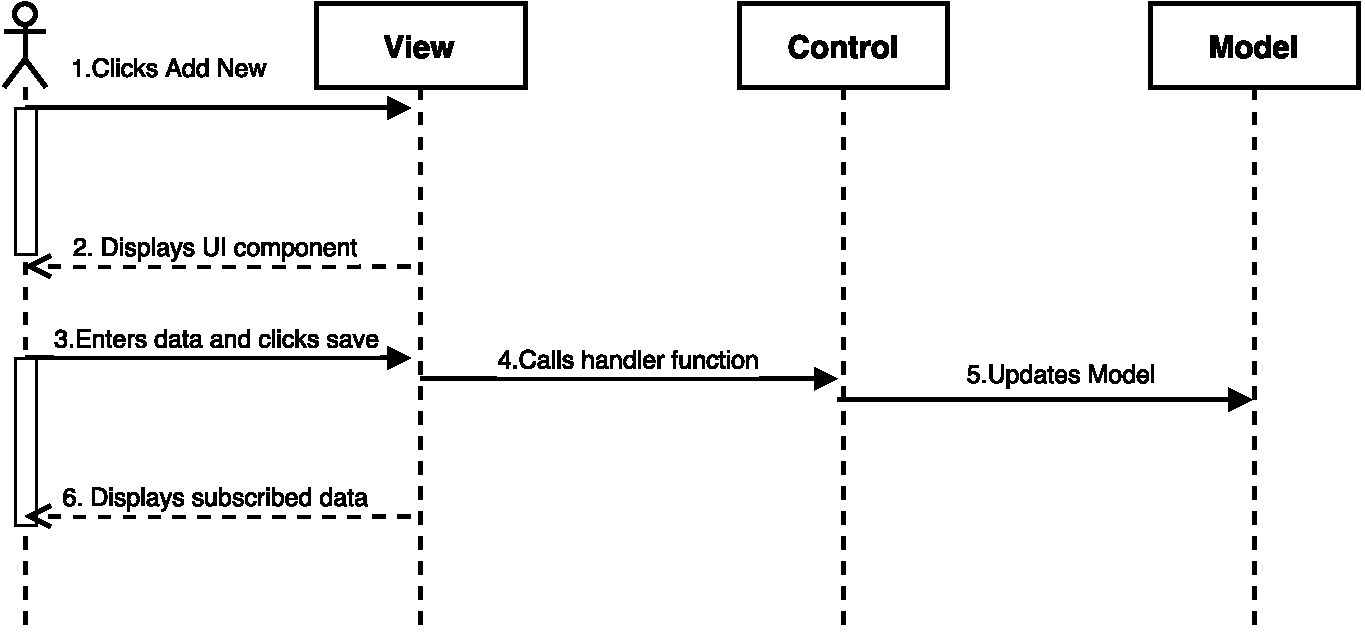
\includegraphics [width= \textwidth]{mvc_pattern.pdf}
	\caption{MVC Pattern of Adding New Entity}
	\label{fig:mvc_pattern}
\end{figure}

\begin{enumerate}
	\item User clicks the \textit{Add New} button in the developed editor.
	\item Responding to the user click, view displays the respective user interface component for entering the new entity data details.
	\item User enters the required basic details for adding new entity data and clicks save button.
	\item View dispatches data to control, as control can only modify the model.
	\item Control inserts/updates data into the model.
	\item View displays the updated model as it has been subscribed to the model.
\end{enumerate}

%%%%%%%%%%%%%%%%%%%%%%%%%%%%%%%%%%%%%%%%%%%%%%%%%%%%%%%%%%%%%%%%%%%%%%%%%
\section{Architecture of the Functioning System}
\label{sec:architectureofthefunctioningsystem}
%%%%%%%%%%%%%%%%%%%%%%%%%%%%%%%%%%%%%%%%%%%%%%%%%%%%%%%%%%%%%%%%%%%%%%%%%
Also from the Figure \ref{fig:architectureofthecasestudy}, it is clear that we followed the MVC architecture to design the user interface. Business experts can use the web-based modeling tool to view/update the descriptive entity details. Whenever a change in the model data is detected respective handler function is \textit{dispatched} and the corresponding handler function can only \textit{update} the model. Since we associate every modeling element with another modeling element, model data of an element is required by another element which are resolved using the unique reference identifier. For example, intention model's unique reference identifier of intention \textit{improve help customer help portal} is required by the strategy \textit{through application development}. This is because, for strategy (through application development), intention (improve help customer help portal) is the target intention. 

\begin{figure}
	\centering
	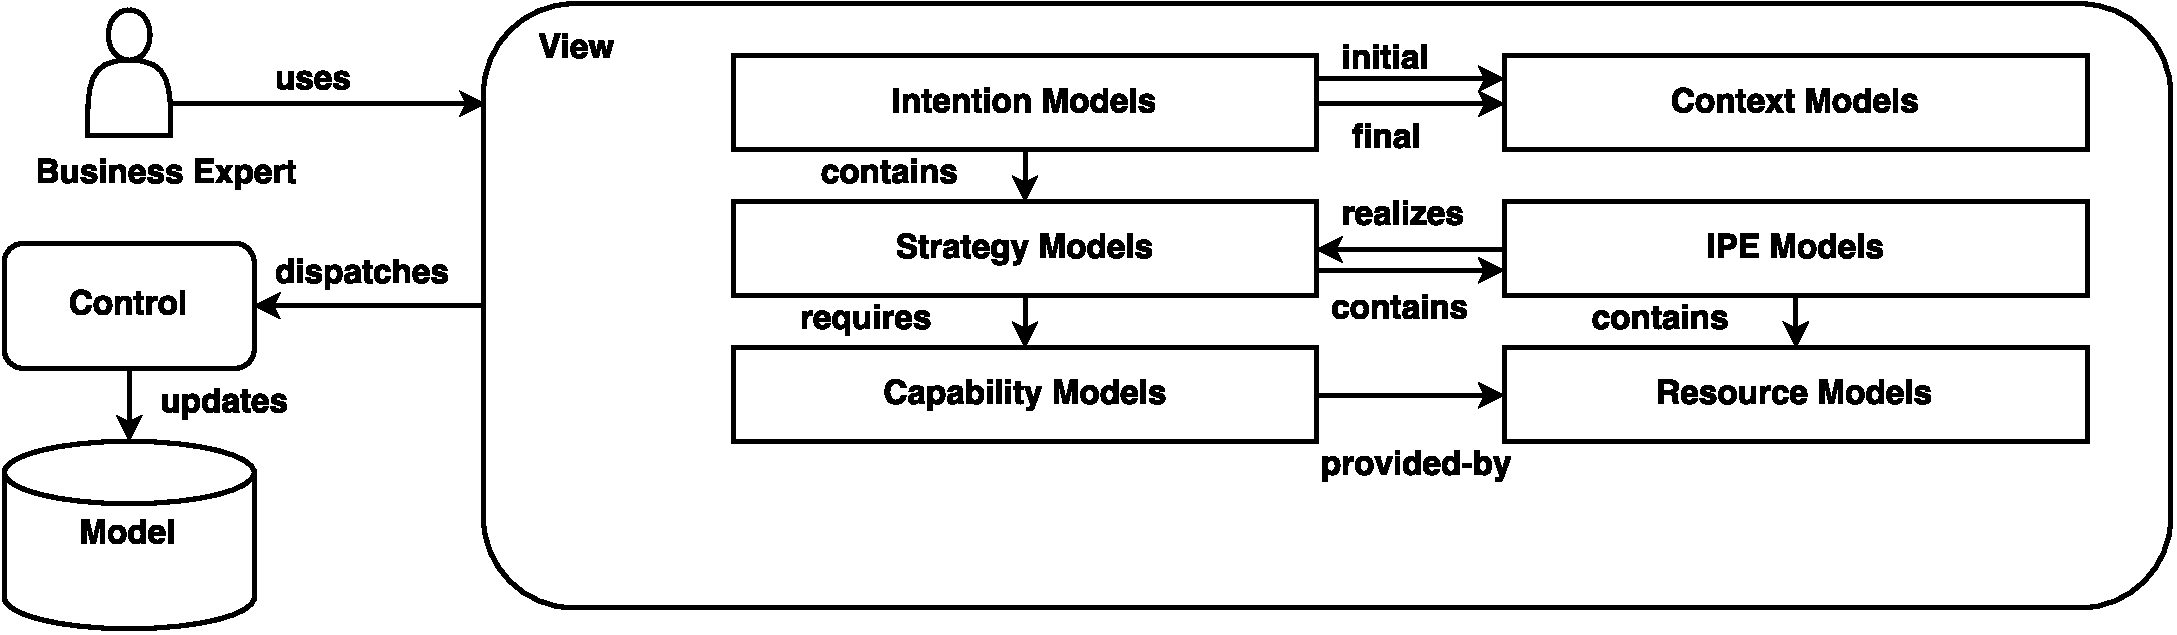
\includegraphics [width= \textwidth]{architectureofthecasestudy.pdf}
	\caption{Architecture of the Functioning System}
	\label{fig:architectureofthecasestudy}
\end{figure}


%%%%%%%%%%%%%%%%%%%%%%%%%%%%%%%%%%%%%%%%%%%%%%%%%%%%%%%%%%%%%%%%%%%%%%%%%
\subsection{Application Flow}
\label{subsec:applicationflow}
%%%%%%%%%%%%%%%%%%%%%%%%%%%%%%%%%%%%%%%%%%%%%%%%%%%%%%%%%%%%%%%%%%%%%%%%%
 In this subsection, we provide an overview about how page navigation from current location to the desired location happens in URL of the browser. The external libraries used for route navigation, parses URL into data structures and generates URL from data structure defined as required routes. We call a function to dispatch route, with the matched route. Then we also have another function that parses the URL, to turn URL into data structure representing it. From the Figure \ref{fig:UIArchitecture}, it is clear that route navigation for each entity items happens based on their entity type and its own unique reference identifier.

\begin{figure}
	\centering
	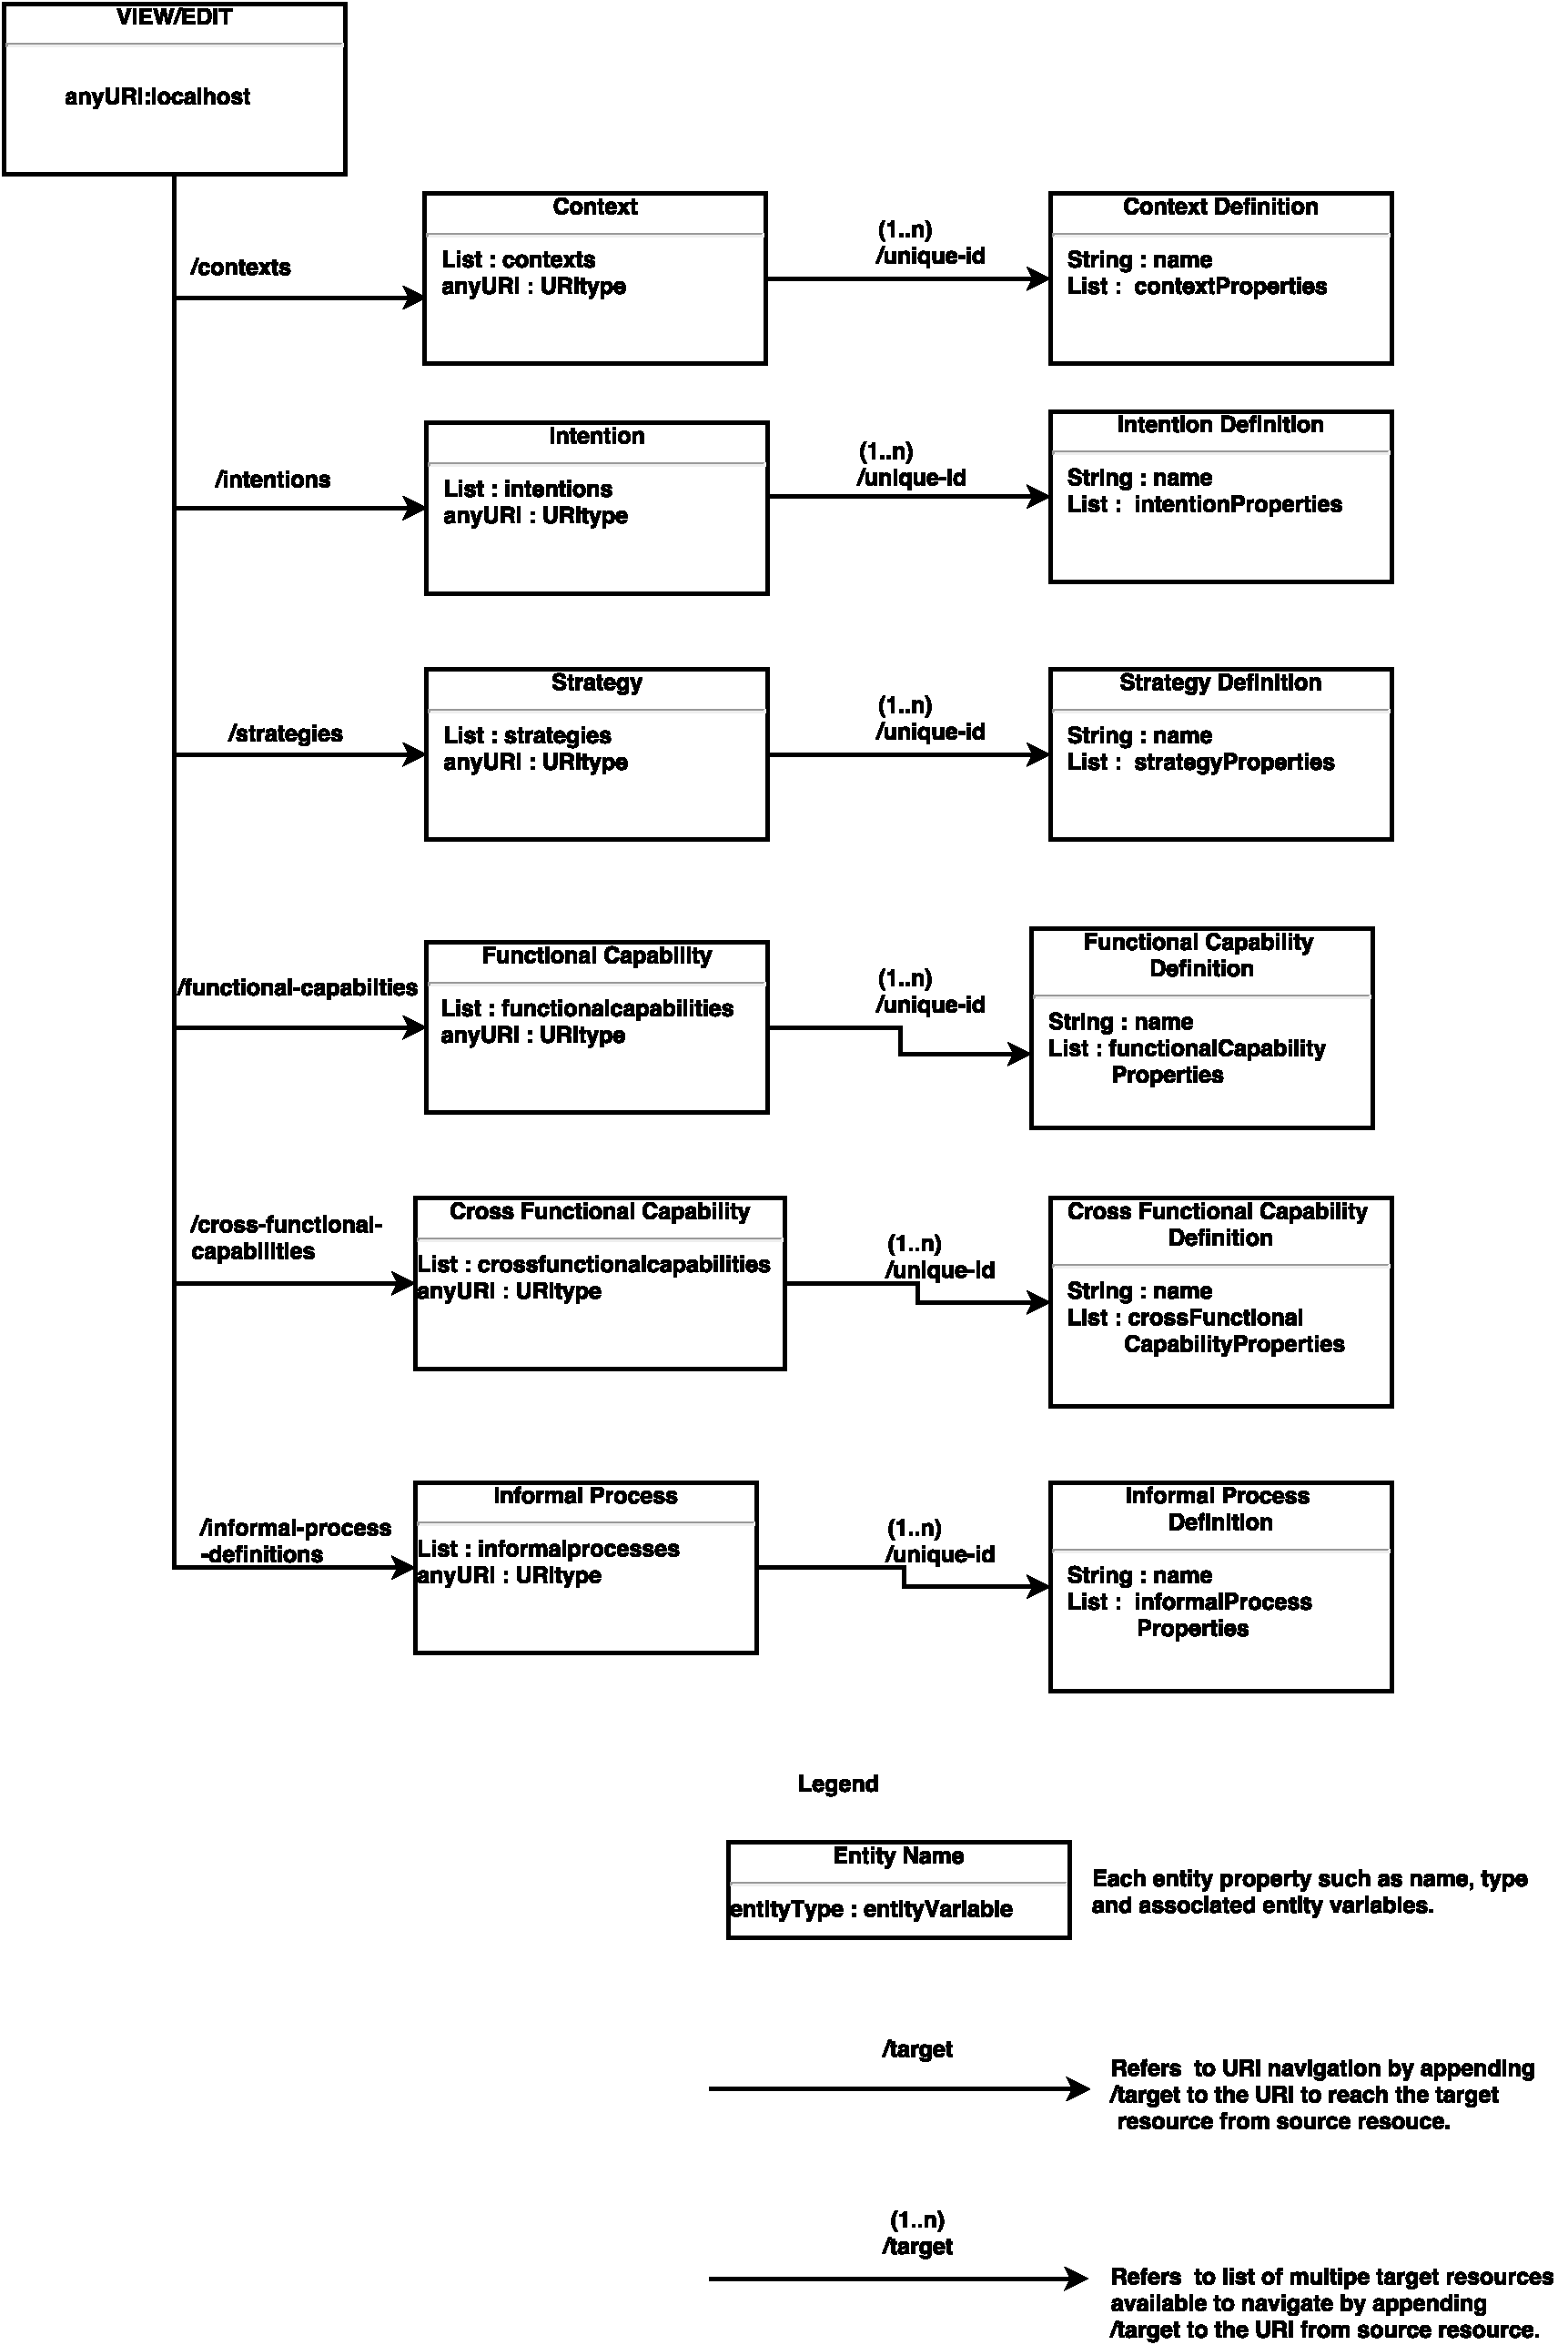
\includegraphics [width= \textwidth]{UIArchitecture.pdf}
	\caption{Implementation of URL Navigation}
	\label{fig:UIArchitecture}
\end{figure} 

Each entity item has basic properties such as \textit{name} and \textit{target namespace}. The entities are identified using their unique id which is generated using the unique combination of name and target namespace. The entities that are associated with a particular entity are resolved through unique identifier. For example, in our motivating scenario consider the intention \textit{improve the customer help desk portal} when creating model for this intention, business expert provide name and namespace for this intention and add it to the database. A unique identifier is generated for the intention model using the combination of name and namespace by the system. For example, the strategy in the motivating scenario \textit{through application  development} that is associated with an intention, contains only the unique identifier of intention as reference. 

%%%%%%%%%%%%%%%%%%%%%%%%%%%%%%%%%%%%%%%%%%%%%%%%%%%%%%%%%%%%%%%%%%%%%%%%%
\section{User Interface Design of the Modeling Tool}
\label{sec:designmethodology}
%%%%%%%%%%%%%%%%%%%%%%%%%%%%%%%%%%%%%%%%%%%%%%%%%%%%%%%%%%%%%%%%%%%%%%%%%
This section discusses in detail the methods followed for designing the web-based modeling tool. The developed tool realizes the approach proposed in the Section \ref{sec:topdownapproach}. When designing the user interface components and functionalities, most of the similar functionalities are designed as common functions for the purpose of reusing the functions. This reduced unnecessary functional redundancies and overhead. It is also important to provide an introduction about the user interface design of the modeling tool, as it helps in understanding the following sections. Also to ensure consistency of the design, all the modeling elements' layout have similar user interface design as follows:



\subsection{Basic Properties}
From the Figure \ref{fig:samplescreen}, we could see that basic properties such as name and target namespace of a modeling element are displayed under the basic properties tab. 

\begin{figure}[H]
	\centering
	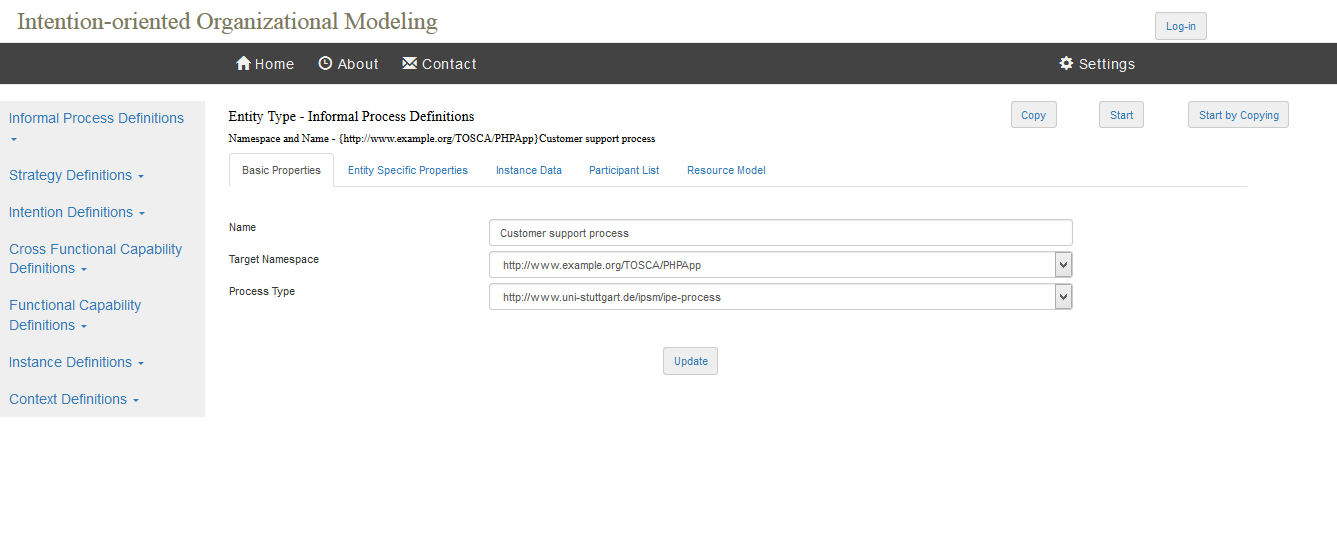
\includegraphics[width=\textwidth,angle=0]{Design_UI.png}
	\caption{User Interface Design of the Basic Properties Tab}
	\label{fig:samplescreen}
\end{figure}

\subsection{Entity Specific Properties}
The entity specific properties of a modeling element are displayed under this tab. The entity specific properties differ from each entity type, i.e., intention, strategy, etc. For example, intention models contain achieving strategies, related intentions, etc., under entity specific properties tab but strategy models contain details like target intentions, required organizational capabilities, etc. From the Figure \ref{fig:samplescreen_esp}, we could see that entity specific properties of a process model includes details of associated contexts, intentions and estimated cost of the process model.

\begin{figure} [H]
	\centering
	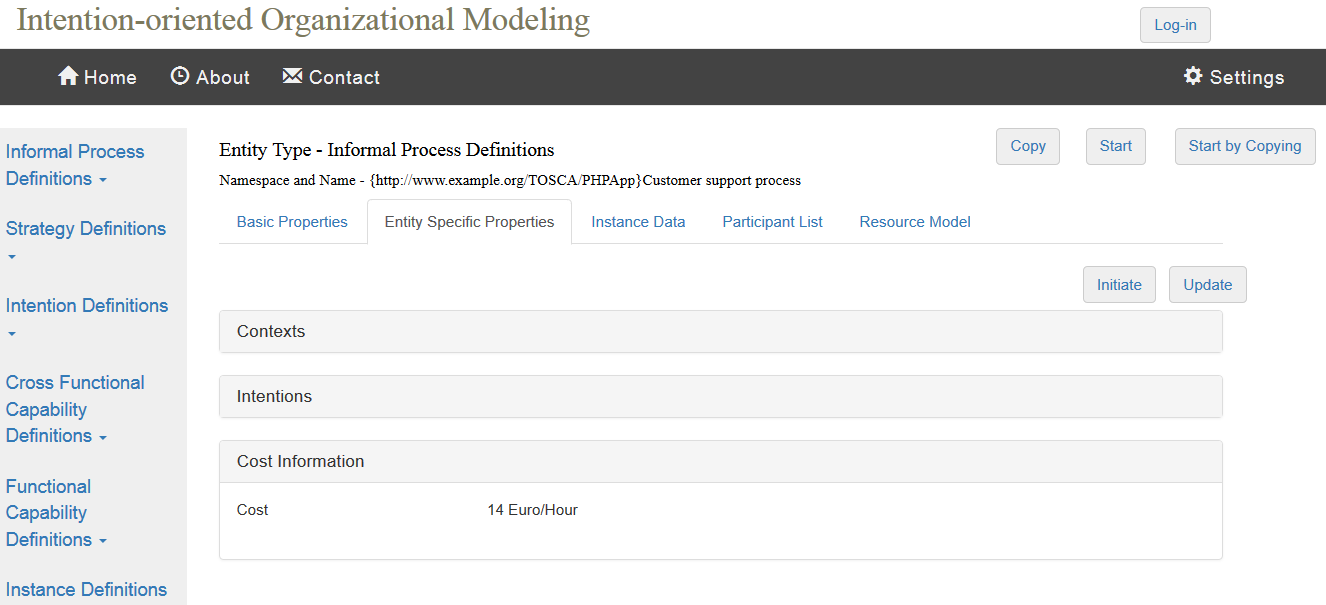
\includegraphics[width=\textwidth,angle=0]{Design_UI_ESP.png}
	\caption{User Interface Design of the Entity Specific Properties Tab}
	\label{fig:samplescreen_esp}
\end{figure}

\subsection{Participant List}
Since intention-oriented organizational modeling satisfies the requirement of participative organizational modeling, we provide participant list tab. This tab holds details of organizational members and their respective privileges. The current design includes only adding and removing of the organizational members as participants. The design also includes assigning privileges to participants such as priviliege to edit, view, follow and own. But the current functioning system, could not check if the members do work based on their privileges. For example, consider a participant who has privilege to only view an intention model and suppose if the participant edits the model then the functioning system does not have functionalities to prevent him from doing so. From the Figure \ref{fig:samplescreen_pl}, we could see that participant list tab of a modeling element contains the details of participants those who can edit, view, follow or own a particular model. 
From thr Figure \ref{fig:samplescreen_pl_editor}, we could see how privileges for a particular participant can be provided and revoked.  
\begin{figure} [H]
	\centering
	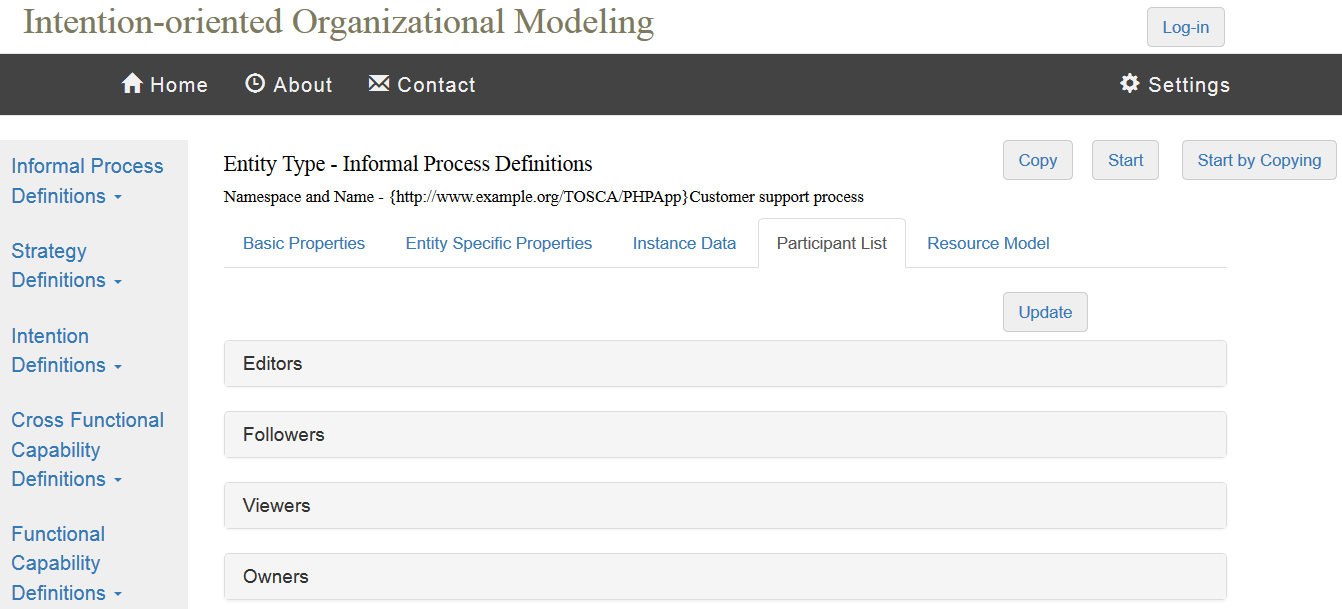
\includegraphics[width=\textwidth,angle=0]{Design_UI_Participant_2.png}
	\caption{User Interface Design of the Participant List Tab}
	\label{fig:samplescreen_pl}
\end{figure}

\begin{figure} [H]
	\centering
	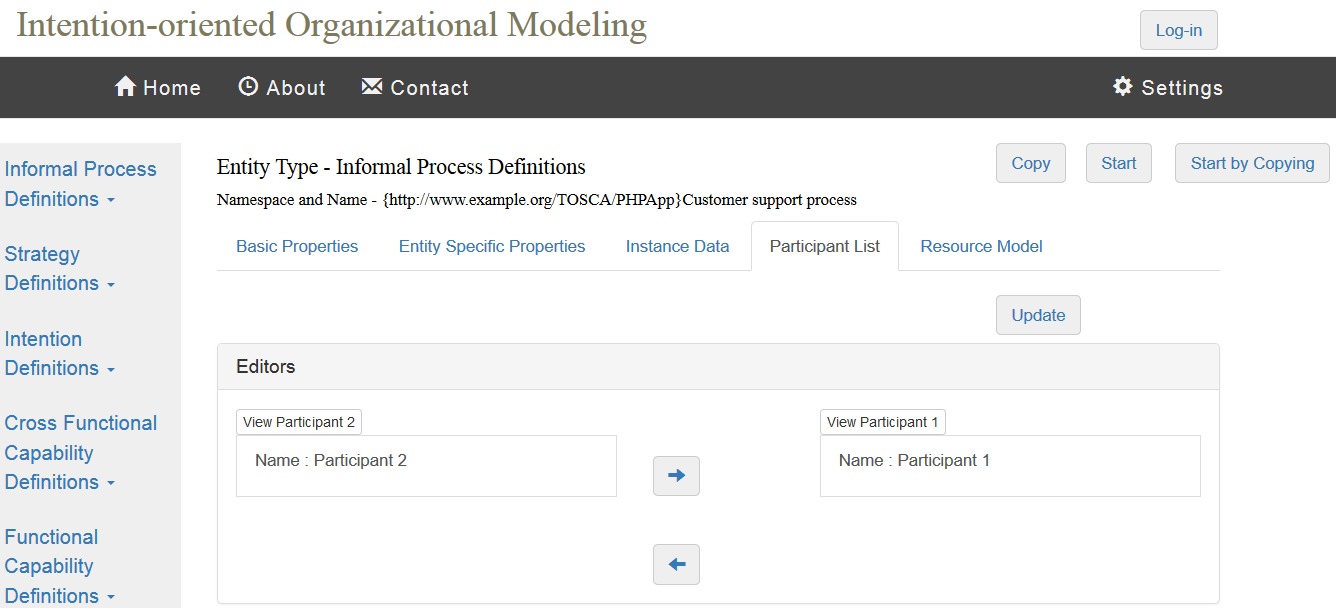
\includegraphics[width=\textwidth,angle=0]{Design_UI_Participant.png}
	\caption{User Interface Design of the Participant as an Editor of the Model}
	\label{fig:samplescreen_pl_editor}
\end{figure}

\subsection{Instance Data}
When a model is initialized, it results in a model instance. As mentioned earlier, a model instance contains additional metadata.
The instances contained under a model are shown inside the instance data tab. For example, the Figure \ref{fig:samplescreen_instance} shows the instance contained under an informal process model. 
  

\begin{figure} [H]
	\centering
	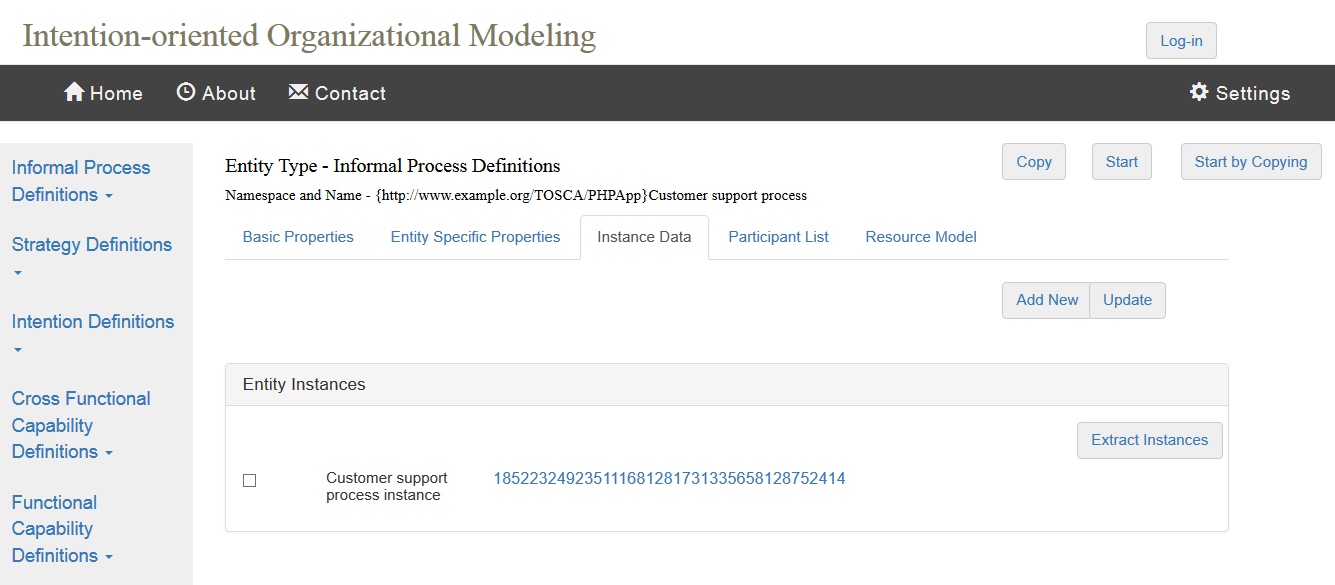
\includegraphics[width=\textwidth,angle=0]{Design_UI_InstanceData.png}
	\caption{User Interface Design of the Instance Data Tab}
	\label{fig:samplescreen_instance}
\end{figure}


Some of the important methodologies followed with respect to user interface components design are (1) multiple items to be selected from multiple list items are displayed as \textit{list group} and (2) selecting single item from multiple items are displayed as \textit{drop down}. For example, to select multiple strategies from a list of strategies, available strategies are displayed as a list from which the user can select desired number of strategies. Another important methodology followed during user interface design is, for every entity the properties should be displayed only under the respective properties tab. For example, in the Figure \ref{fig:samplescreen}, the basic properties such as name, target namespace and process type of an informal process model should be displayed only under the respective basic properties tab and similarly for all other tabs. This methodology is followed uniformly throughout the design of all the entity types such as intention definitions, strategy definitions, capability definitions, context definitions, instance definitions and informal process definitions. 

All data are stored only under the data artifact. This applies to the labels and text fields of all user interface elements and this data can be updated only through the handler function. Through the \textit{settings} option, user can add new namespace type and intention relation type. From the Figure \ref{fig:samplescreen}, it is clear that a consistent design methodology has been followed to display the list of available entity types such as intentions, strategies, capabilities etc., and to display their respective properties such as basic, entity specific, instance data, etc., properties. Though the top-down modeling approach \ref{sec:topdownapproach}, shows that definition of each entity type is contained within another entity type, as per the user interface design, separate entities references each other using the unique reference identifier but does not contain all properties of referenced entity. For instance, a strategy containing an intention should contain only the intention's unique reference identifier but not the actual intention itself. Later in the view of strategy, actual intention properties are fetched and displayed based on the unique reference identifier. 


%%%%%%%%%%%%%%%%%%%%%%%%%%%%%%%%%%%%%%%%%%%%%%%%%%%%%%%%%%%%%%%%%%%%%%%%%
\section{Realization of the Approach}
\label{sec:realization}
%%%%%%%%%%%%%%%%%%%%%%%%%%%%%%%%%%%%%%%%%%%%%%%%%%%%%%%%%%%%%%%%%%%%%%%%%
In order to realize the proposed approach in the Section \ref{sec:topdownapproach} of Chapter \ref{chap:approach}, we create models using the developed web-based modeling tool for the motivating scenario discussed in the Chapter \ref{chap:motivatingScenario}. It is also important to model them step by step as mentioned in the Section \ref{chap:approach}. As we mentioned earlier, to realize the approach in organizations, we model the motivating scenario step by step as mentioned in the second phase of the InProXec method. The step of modeling are discussed in the Section \ref{sec:informalprocessmodeling} of previous Chapter \ref{chap:approach}. As each models are designed in an individual modeling step, details of individual modeling steps are provided in the following subsections. 

%%%%%%%%%%%%%%%%%%%%%%%%%%%%%%%%%%%%%%%%%%%%%%%%%%%%%%%%%%%%%%%%%%%%%%%%%
\subsection{Modeling of Contexts}
%%%%%%%%%%%%%%%%%%%%%%%%%%%%%%%%%%%%%%%%%%%%%%%%%%%%%%%%%%%%%%%%%%%%%%%%%
In the informal process modeling approach, the first modeling step is to model the context definitions (M1). Each informal process starts from an initial context and aims to achieve an intention \cite{Sungur2014a}. After reaching an intention, there is resulting IPE Context. To realize the motivating scenario, user can add new contexts by providing basic properties such as name of the context and target namespace of the context as they serve as unique reference identifier for these contexts. After successfully adding the basic properties, user can provide entity specific properties such as contained contexts inside the main context, entity definition details about the contexts and participant list with respective privileges for each participant are also provided. The required context definitions are modeled first because these definition are required for modeling intention definitions and process definitions.  

%%%%%%%%%%%%%%%%%%%%%%%%%%%%%%%%%%%%%%%%%%%%%%%%%%%%%%%%%%%%%%%%%%%%%%%%%
\subsection{Modeling of Intentions}
%%%%%%%%%%%%%%%%%%%%%%%%%%%%%%%%%%%%%%%%%%%%%%%%%%%%%%%%%%%%%%%%%%%%%%%%%
After modeling context definitions(M1), the second step of the modeling is to model the intentions (M2). For example, in our motivating scenario we have main intention as "increase revenue and number of unit sales" and other low level intentions that emerged out of main intention and strategies of the main intention. The user can provide descriptive information about particular intention as intention definition. Similar to context modeling, the user has to provide basic properties such as name and target namespace required for unique identification of the entity. After providing basic properties, the user has to provide entity specific details of the intention such as due date and time for intention completion, priority of the intention, cost of the intention, other related intentions that are contained under this particular intention. The strategies to achieve this intention and contexts of the intention are also provided as entity specific properties. The participant list with respective privileges for each participant are also provided when an entity is of type interactive acquirable entity. 

%%%%%%%%%%%%%%%%%%%%%%%%%%%%%%%%%%%%%%%%%%%%%%%%%%%%%%%%%%%%%%%%%%%%%%%%%
\subsection{Modeling of Strategies}
%%%%%%%%%%%%%%%%%%%%%%%%%%%%%%%%%%%%%%%%%%%%%%%%%%%%%%%%%%%%%%%%%%%%%%%%%
After modeling context definitions (M1) and intention definitions (M2) user can proceed to model the strategies (M3) which is third step of the modeling process. For example, in our motivating scenario user can model the strategies such as \textit{through expansion}, \textit{through advertisements} and other required strategies as third step of the modeling process. Similar to earlier modeling steps, during modeling of strategy user required to provide basic properties such as name and target namespace. After providing the basic properties, entity specific properties such as target intentions of the strategy, capabilities and process definitions associated with strategy are also provided. Since, strategy is also an interactive acquirable entity similar to intention, participant list details are also provided during modeling of strategies

%%%%%%%%%%%%%%%%%%%%%%%%%%%%%%%%%%%%%%%%%%%%%%%%%%%%%%%%%%%%%%%%%%%%%%%%%
\subsection{Modeling of Capabilities}
%%%%%%%%%%%%%%%%%%%%%%%%%%%%%%%%%%%%%%%%%%%%%%%%%%%%%%%%%%%%%%%%%%%%%%%%%
Modeling of capability (M4) is the fourth step in intention-oriented organizational modeling. There are two types of capabilities. Functional capabilities and cross-functional capabilities. Functional capabilities are the capabilites that associated with other entity types. Cross-functional capabilities contains multiple functional capabilities. Similar to earlier entity types' basic properties such as name and target namespace are added to get the unique reference identifier and entity specific properties for capabilities are added. Since cross functional capability contains functional capabilities, it holds the identifiers of the functional capabilities contained in it. Functional capability definitions also has participant list details similar to intention definitions and strategy definitions. 


%%%%%%%%%%%%%%%%%%%%%%%%%%%%%%%%%%%%%%%%%%%%%%%%%%%%%%%%%%%%%%%%%%%%%%%%%
\subsection{Modeling of Resources}
%%%%%%%%%%%%%%%%%%%%%%%%%%%%%%%%%%%%%%%%%%%%%%%%%%%%%%%%%%%%%%%%%%%%%%%%%
Each resource that provides certain capability can be related to another resource which are defined using predefined or custom \textit{relationships} \cite{Sungur2014a}. These resources are managed through \textit{resource organizers}, this is because resource organizers are used to bring together the relevant interrelated resources that work towards to achieve an intention. TOSCA \cite{Binz2014} can be used to model all nodes and relationship among them. In this work, authors consider resources as nodes to make use of the TOSCA's service. In the developed modeling tool, the resource models are managed by embedding the open source modeling tool Winery web page \cite{Kopp2013} in the modeling tool's web page. This is because it creates a new service template that contains an application topology by using the topology modeler. Winery also offers all available node types in a palette. From there, user can drag the desired node type and drop it into the editing area. There the node type becomes a node template i.e., a node in the topology graph. Node templates can be annotated with requirements and capabilities, property values, and policies.

In order to achieve this, we use TOSCA repository URL referring to winery and topology modeler of the winery. Using these values we create corresponding URL required for our modeling based on the name and namespace properties of an entity. 

%%%%%%%%%%%%%%%%%%%%%%%%%%%%%%%%%%%%%%%%%%%%%%%%%%%%%%%%%%%%%%%%%%%%%%%%%
\subsection{Additional Features of the Tool}
%%%%%%%%%%%%%%%%%%%%%%%%%%%%%%%%%%%%%%%%%%%%%%%%%%%%%%%%%%%%%%%%%%%%%%%%%		
Initializing resource-centric processes require acquiring and engaging interrelated resources \cite{Sungur2015}. As mentioned earlier, the phases of compiling and initializing of informal process models are not within scope of this work. Only the functionalities such as creating instances, extracting instances and editing instances are part of the functioning tool. This is because initializing informal process models starts after the initial context defined in an IPE model \cite{Sungur2015}. Thus, it is important to discuss realization of instance creation which are required for phase P3 of Executing Informal Processes (InProXec) method. Acquirable entity types' models can be converted into instances. For example, process definition is converted into \textit{process instance} when the model is compiled and engaged with resources. A model instance contains additional meta-data about the executed processes such as the information about the start date and time, end date and time, instance status, cost, source model etc. From the screen-shot image \ref{fig:realizationofinstances2} it is clear that these properties of an instance can be edited through the developed tool. Only when a acquirable model is successfully initialized it can be engaged to adapt the process execution of emerging requirements \cite{Sungur2015}. 

The developed tool supports creation and updation of descriptive information about instances. Each instance belong to any one of the acquirable entity type such strategies, intentions and informal processes. Any entity that has instances are also listed inside the \textit{Instance data} tab of each entity. From the user interface screen Figure \ref{fig:realizationofinstances}, it is clear that the editor has ability to add, remove and extract instance descriptors for any entity type. An instance descriptor of a functional capability refers to a resource definition meaning that a capability is provided by a resource.
 
\begin{figure} [H]
	\centering
	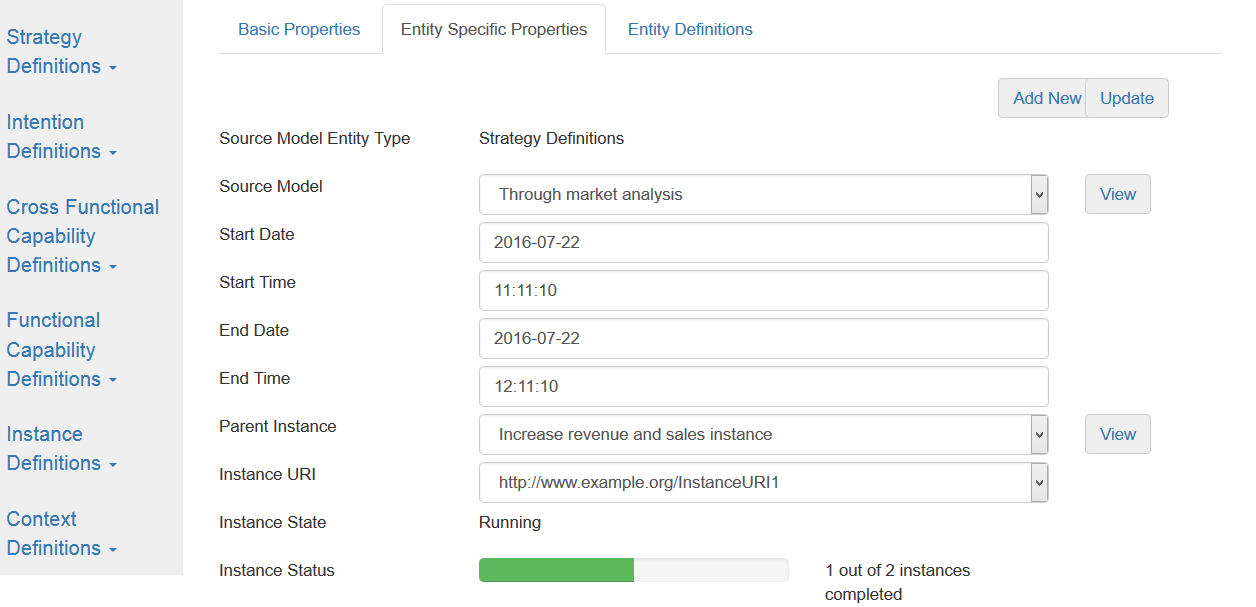
\includegraphics[width=\textwidth,angle=0]{Design_UI_Instance.png}
	\caption{User Interface Screen of an Instance Model}
	\label{fig:realizationofinstances}
\end{figure}

		
%%%%%%%%%%%%%%%%%%%%%%%%%%%%%%%%%%%%%%%%%%%%%%%%%%%%%%%%%%%%%%%%%%%%%%%%%
\section{Realization of the Requirements}
\label{sec:validation}
%%%%%%%%%%%%%%%%%%%%%%%%%%%%%%%%%%%%%%%%%%%%%%%%%%%%%%%%%%%%%%%%%%%%%%%%%	
This section provides details of realizing the requirements of intention-oriented organizational modeling that are satisfied by the proposed approach. 

\textit{Organizational Intention Transparency} (R1):  Using the modeling tool intentions at different levels can be modeled which satisfies first pre-requisite of R1. With the current functioning system any user can view intention at different levels which satisfies second pre-requisite of R2. Thus, requirement R1 is satisfied by the functioning system as both of its pre-requisites are satisfied .

\textit{Organizational Strategy-based Cost Estimation} (R2): The modeling tool itself calculates and displays the estimated strategy cost calculation based on strategy implementation and resource cost. This cost information helps the business experts to make certain decision based on cost calculation during modeling. The functioning tool satisfies requirement R2 as both of its pre-requisites are met by the tool. 

\textit{Organizational Strategy Achievability Estimation} (R3): Similar to cost calculation, strategy achievability estimation based on its association with valid capability is also determined and displayed during modeling phase itself. The functioning tool satisfies requirement R3 as both of its pre-requisites are met by the tool.

\textit{Intention Oriented Working Style} (R4): Any user can create intention models, strategy models, informal process models etc., through the developed tool provided the user has understanding about main intention and its recursive structure. The requirement R4 is also satisfied by the functioning tool as it satisfies both the pre-requisites of R4.

\textit{Participative Organizational Modeling} (R5): Each entity type that can be interactively acquirable has list of participants with their corresponding privileges. The users can edit, view, own or follow based on their privilege. Thus, the tool satisfies the requirement R5.


\cleardoublepage
\chapter{Conclusion and Future Work}
\label{chap:conclusion}

In this document, we first started Chapter \ref{chap:introduction} with motivational and problem statement followed by contributions of this work. In Chapter \ref{chap:fundamentals}, the fundamental concepts and related work from existing literature has been provided in detail. In Chapter \ref{chap:motivatingScenario}, a motivating scenario has been taken and explained based on the guidelines and real life scenarios discussed in some previous work. In Chapter \ref{chap:analysis}, a detailed requirements analysis based on existing literatures, a motivating scenario and evaluation of existing approaches has been provided. This is followed by Chapter \ref{chap:approach}, which provides an approach that satisfies all of the derived requirements. A detailed case study has been provided in Chapter \ref{chap:casestudy}, which helps to assess feasibility of the proposed approach. This chapter also validates the developed web–based modeling tool by providing examples that satisfies the derived requirements discussed in Chapter \ref{chap:analysis} and also conformance of the motivating scenario discussed in Chapter \ref{chap:motivatingScenario} with the developed system.

This work provides an approach that satisfies all of the requirements of intention-oriented organizational modeling and realized the proposed approach as a web-based modeling tool. The models developed through this approach act as a complementary informal guides and definitions required for intention-oriented organizational modeling. 

%%%%%%%%%%%%%%%%%%%%%%%%%%%%%%%%%%%%%%%%%%%%%%%%%%%%%%%%%%%%%%%%%%%%%%%%%
\section*{Future Work}
\label{sec:futurework}
%%%%%%%%%%%%%%%%%%%%%%%%%%%%%%%%%%%%%%%%%%%%%%%%%%%%%%%%%%%%%%%%%%%%%%%%%
The web-based modeling tool developed as a part of this master thesis work will be integrated with back end such that it can generate deployable entities from the current descriptive information. The future work also includes providing mobile modeling approach, enabling logging in functionality through few of the popular social network accounts and enhancing the user interface features of the modeling tool. 






%
%
%\renewcommand{\appendixtocname}{Anhang}
%\renewcommand{\appendixname}{Anhang}
%\renewcommand{\appendixpagename}{Anhang}
\appendix
%% !TeX spellcheck = de_DE
%Die Angabe des schlauen Spruchs auf diesem Wege funtioniert nur,
%wenn keine Änderung des Kapitels mittels den in preambel/chapterheads.tex
%vorgeschlagenen Möglichkeiten durchgeführt wurde.
\setchapterpreamble[u]{%
\dictum[Albert Einstein]{Probleme kann man niemals mit derselben Denkweise lösen, durch die sie entstanden sind.}
}
\chapter{LaTeX-Tipps}
\label{chap:latextipps}

\section{File-Encoding und Unterstützung von Umlauten}
Die Vorlage wurde 2010 auf UTF-8 umgestellt.
Alle neueren Editoren sollten damit keine Schwierigkeiten haben.

\section{Zitate}
Referenzen werden mittels \texttt{\textbackslash cite[key]} gesetzt.
Beispiel: \cite{WSPA} oder mit Autorenangabe: \citet{WSPA}.

Wörter am besten mittels \texttt{\textbackslash enquote\{...\}} \enquote{einschließen}, dann werden die richtigen Anführungszeichen verwendet.

\section{Mathematische Formeln}
\label{sec:mf}
Mathematische Formeln kann man $so$ setzen. \texttt{symbols-a4.pdf} (zu finden auf \url{http://www.ctan.org/tex-archive/info/symbols/comprehensive/symbols-a4.pdf}) enthält eine Liste der unter LaTeX direkt verfügbaren Symbole.
Z.\,B.\ $\mathbb{N}$ für die Menge der natürlichen Zahlen.
Für eine vollständige Dokumentation für mathematischen Formelsatz sollte die Dokumentation zu \texttt{amsmath}, \url{ftp://ftp.ams.org/pub/tex/doc/amsmath/} gelesen werden.

Folgende Gleichung erhält keine Nummer, da \texttt{\textbackslash equation*} verwendet wurde.
\begin{equation*}
x = y
\end{equation*}

Die Gleichung~\ref{eq:test} erhält eine Nummer:
\begin{equation}
\label{eq:test}
x = y
\end{equation}

Eine ausführliche Anleitung zum Mathematikmodus von LaTeX findet sich in \url{http://www.ctan.org/tex-archive/help/Catalogue/entries/voss-mathmode.html}.

\section{Quellcode}
\Cref{lst:ListingANDlstlisting} zeigt, wie man Programmlistings einbindet.
Mittels \texttt{\textbackslash lstinputlisting} kann man den Inhalt direkt aus Dateien lesen.

%Listing-Umgebung wurde durch \newfloat{Listing} definiert
\begin{Listing}
\begin{lstlisting}
<listing name="second sample">
  <content>not interesting</content>
</listing>
\end{lstlisting}
\caption{lstlisting in einer Listings-Umgebung, damit das Listing durch Balken abgetrennt ist}
\label{lst:ListingANDlstlisting}
\end{Listing}

Quellcode im \lstinline|<listing />| ist auch möglich.

\section{Abbildungen}
Die Abbildungen~\ref{fig:chor1} und~\ref{fig:chor2} sind für das Verständnis dieses Dokuments wichtig.
Im Anhang zeigt \vref{fig:AnhangsChor} erneut die komplette Choreographie.

%Die Parameter in eckigen Klammern sind optionale Parameter - z.B. [htb!]
%htb! bedeutet: "Liebes LaTeX, bitte platziere diese Abbildung zuerst hier ("_h_ere"). Falls das nicht funktioniert, dann bitte oben auf der Seite ("_t_op"). Und falls das nicht geht, bitte unten auf der Seite ("_b_ottom"). Und bitte, bitte bevorzuge hier und oben, auch wenn's net so optimal aussieht ("!")
%Diese sollten nach Möglichkeit NICHT verwendet werden. LaTeX's Algorithmus für das Platzieren der Gleitumgebung ist schon sehr gut!
\begin{figure}
  \centering
  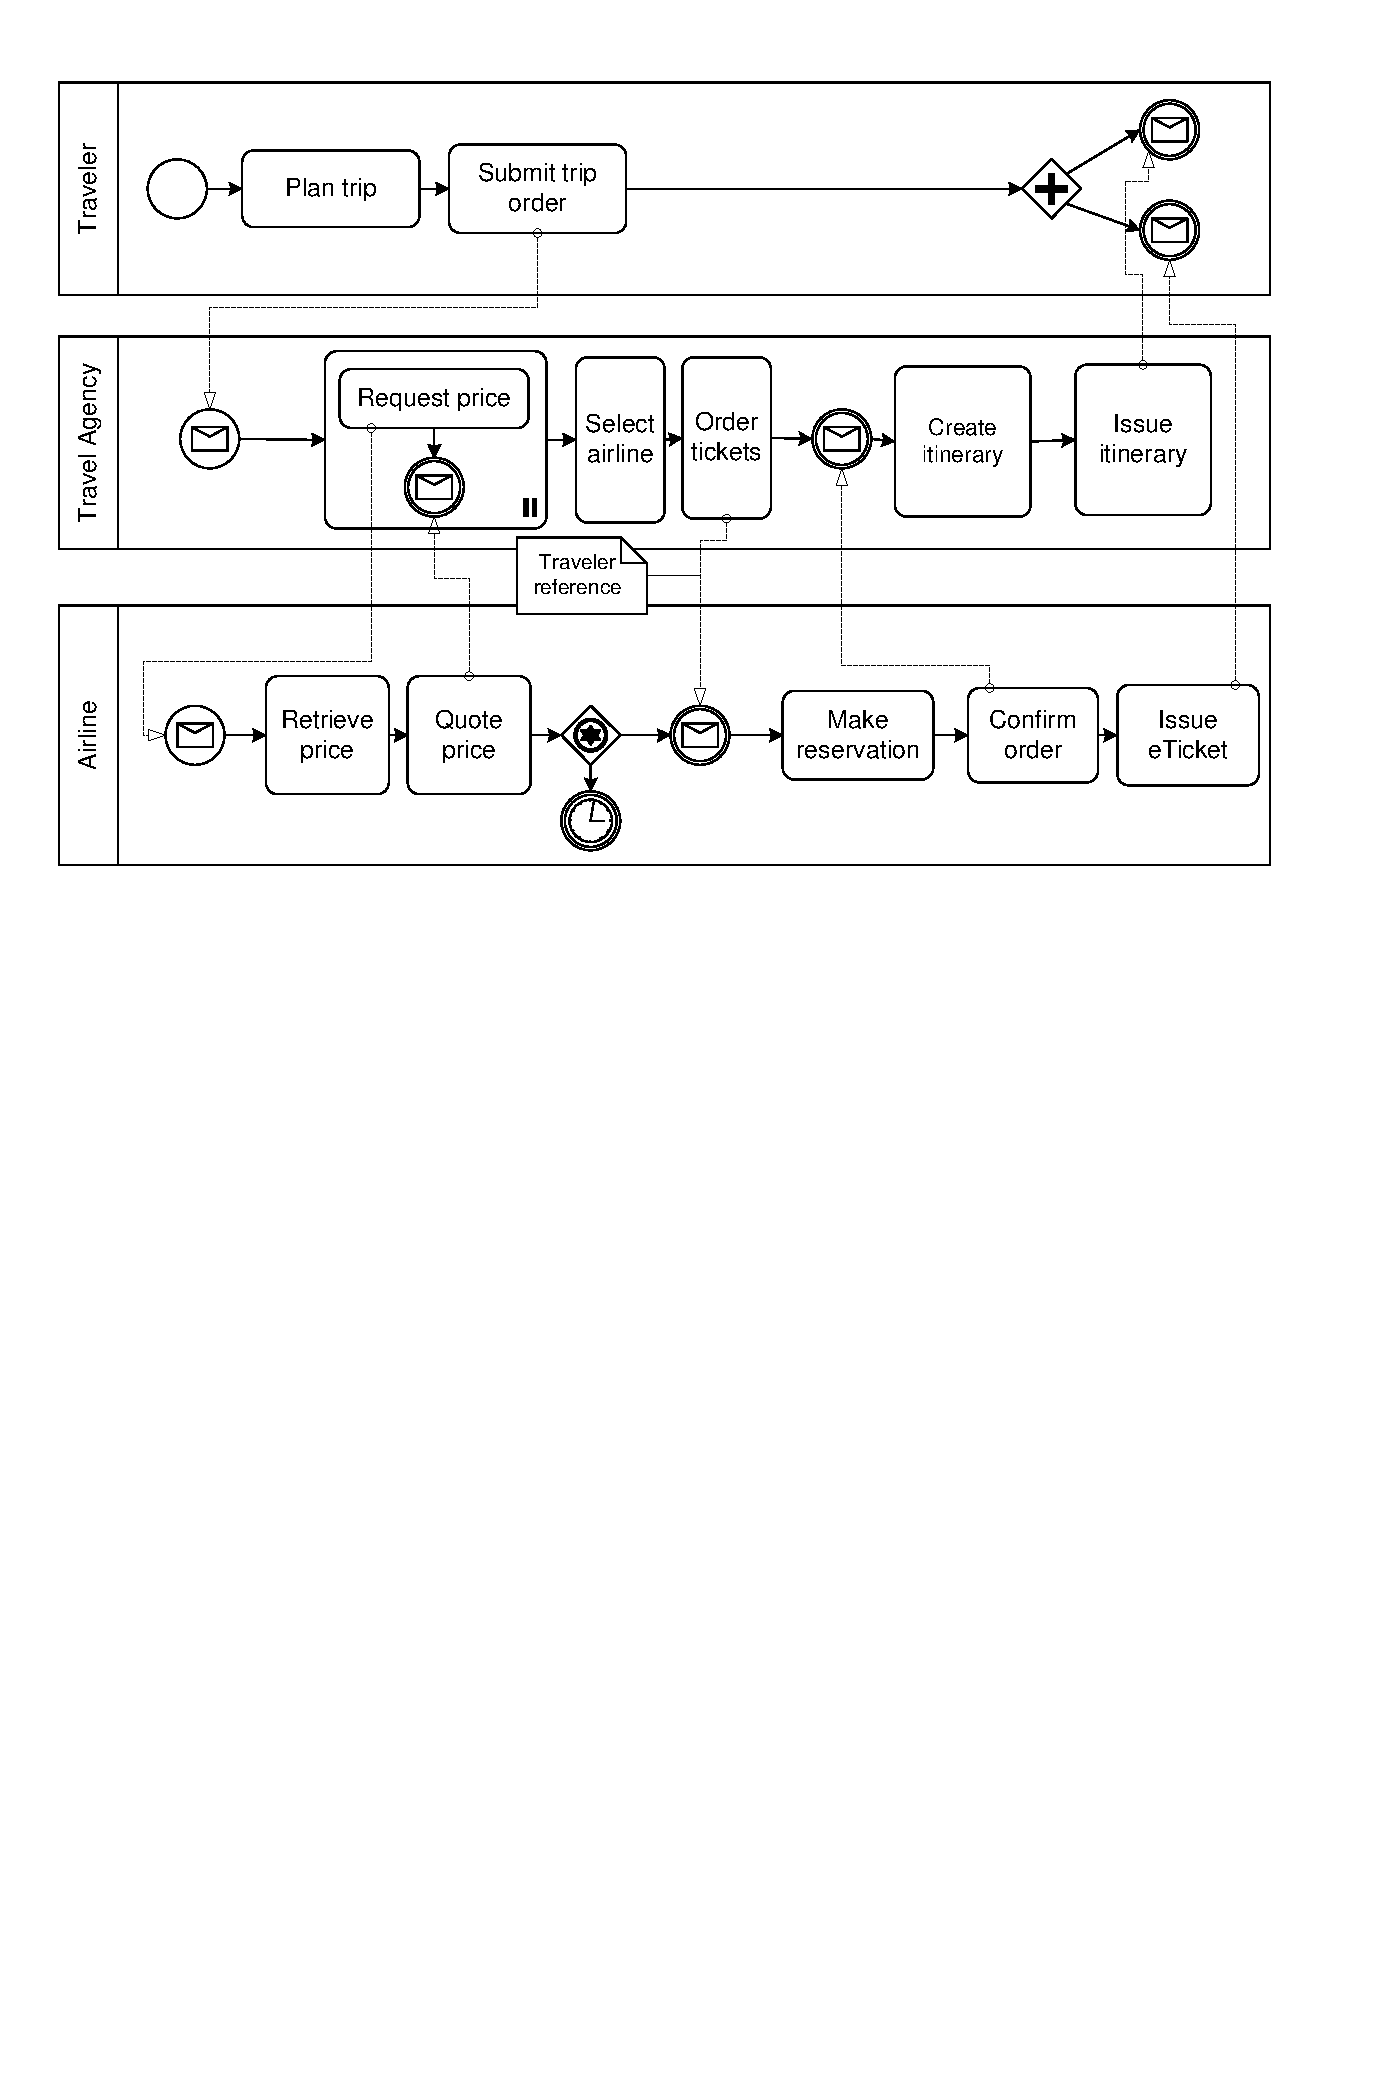
\includegraphics[width=\textwidth]{choreography.pdf}
  \caption{Beispiel-Choreographie}
  \label{fig:chor1}
\end{figure}

\begin{figure}
  \centering
  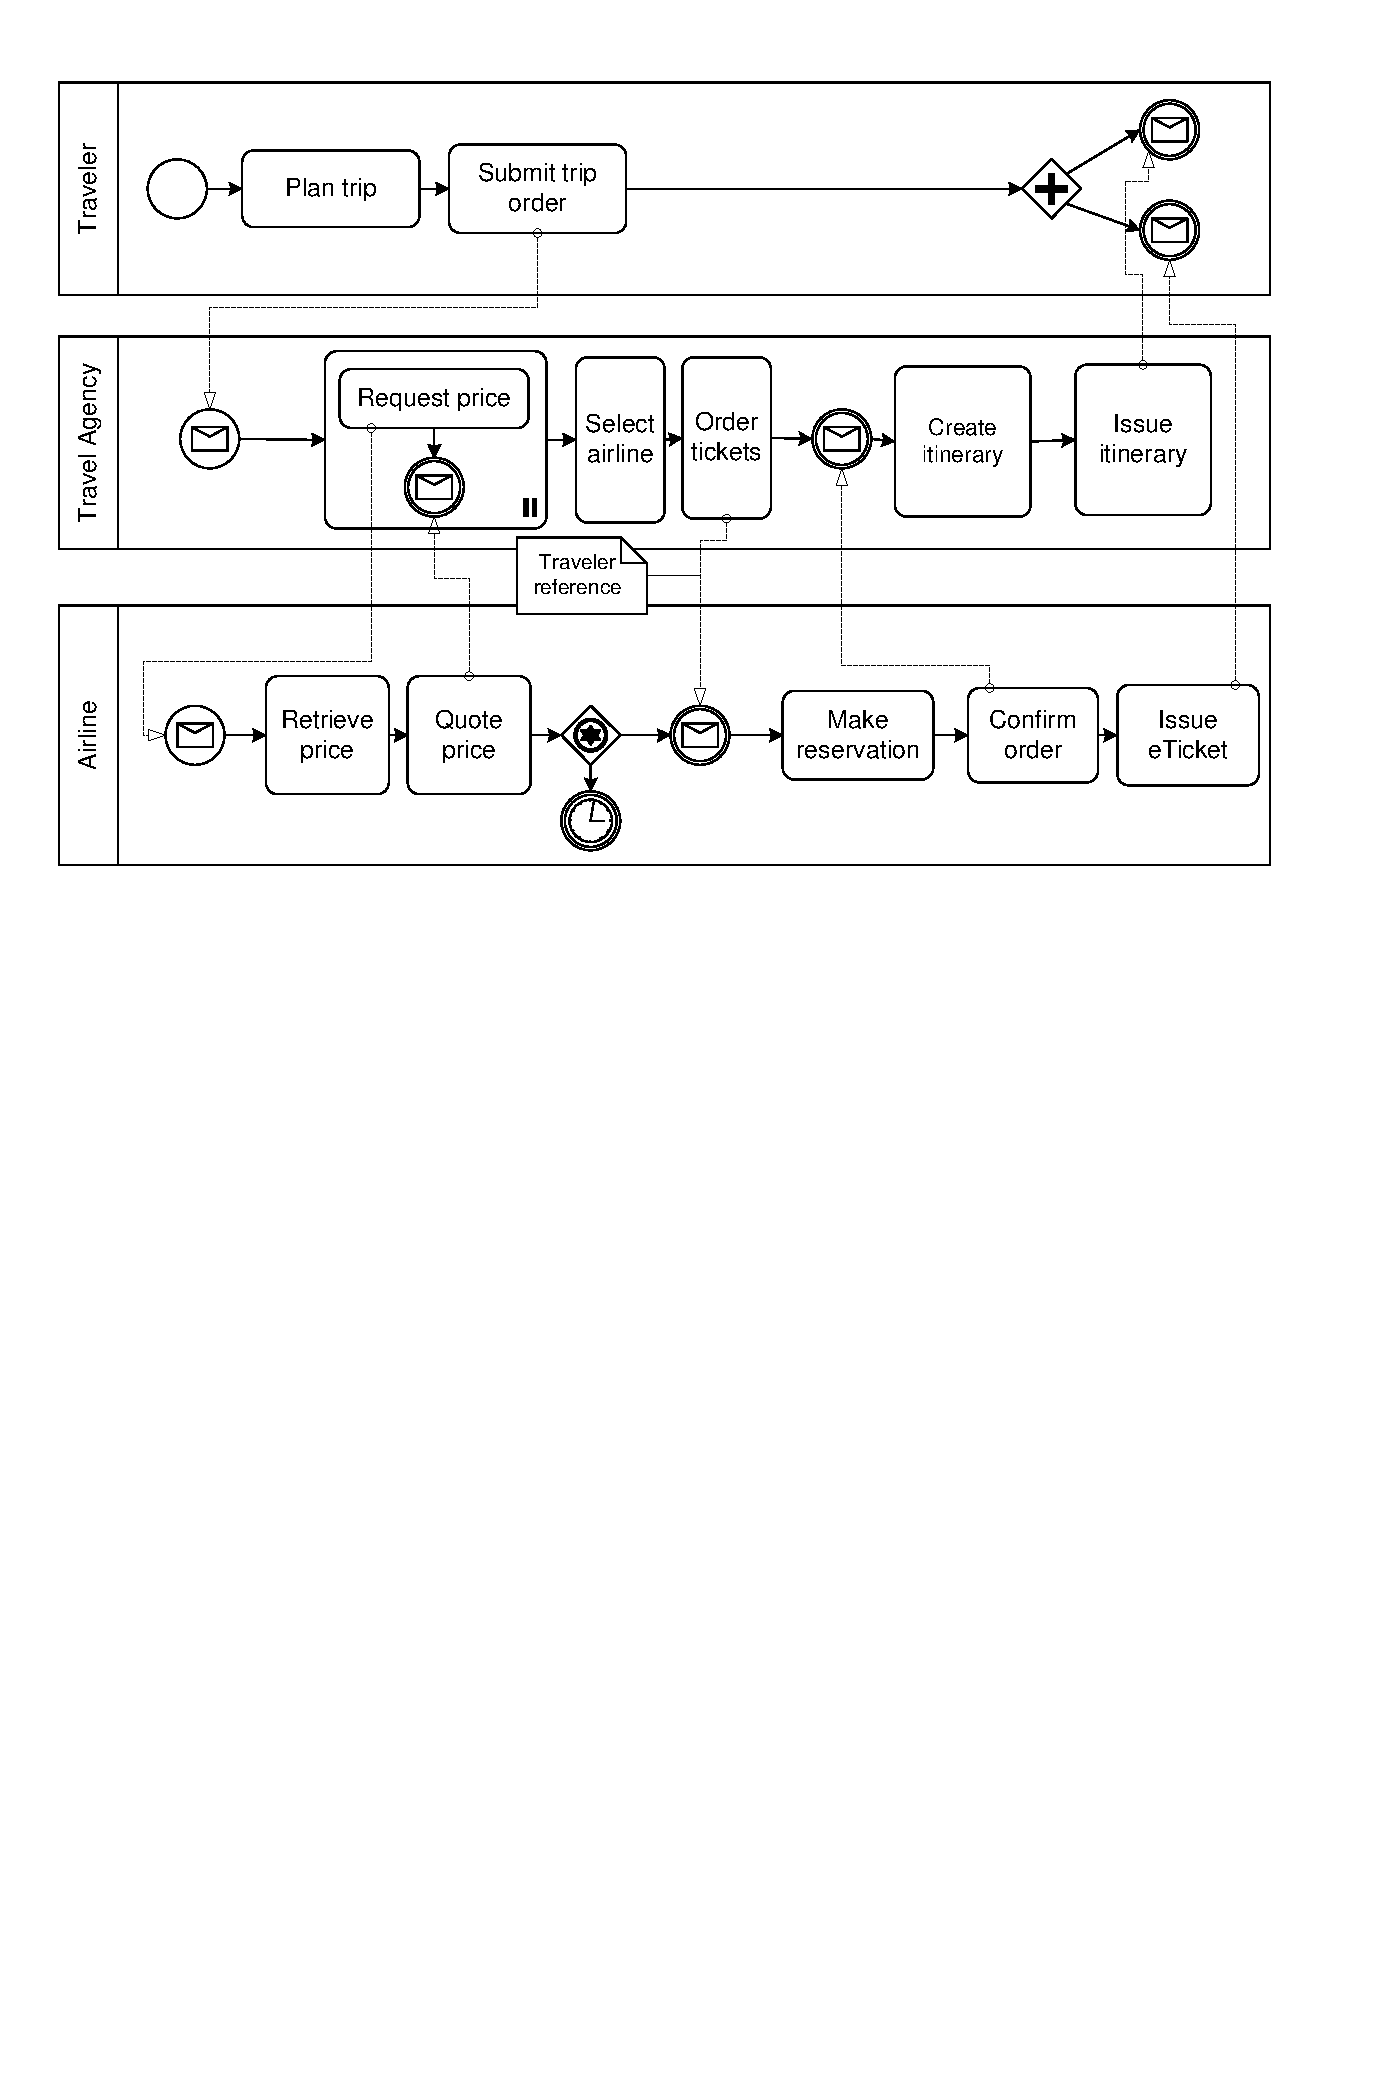
\includegraphics[width=.8\textwidth]{choreography.pdf}
  \caption[Beispiel-Choreographie]{Die Beispiel-Choreographie. Nun etwas kleiner, damit \texttt{\textbackslash textwidth} demonstriert wird. Und auch die Verwendung von alternativen Bildunterschriften für das Verzeichnis der Abbildungen. Letzteres ist allerdings nur Bedingt zu empfehlen, denn wer liest schon so viel Text unter einem Bild? Oder ist es einfach nur Stilsache?}
  \label{fig:chor2}
\end{figure}

Das SVG in \cref{fig:directSVG} ist direkt eingebunden, während der Text im SVG in \cref{fig:latexSVG} mittels pdflatex gesetzt ist.
\todo{Falls man die Graphiken sehen möchte, muss inkscape im PATH sein und im Tex-Quelltext \texttt{\textbackslash{}iffalse} und \texttt{\textbackslash{}iftrue} auskommentiert sein.}

\iffalse % <-- Das hier wegnehmen, falls inkscape im Pfad ist
\begin{figure}
\centering

\includegraphics{svgexample.svg}
\caption{SVG direkt eingebunden}
\label{fig:directSVG}
\end{figure}

\begin{figure}
\centering
\def\svgwidth{.4\textwidth}
\includesvg{svgexample}
\caption{Text im SVG mittels \LaTeX{} gesetzt}
\label{fig:latexSVG}
\end{figure}
\fi % <-- Das hier wegnehmen, falls inkscape im Pfad ist

\section{Tabellen}
Tabelle~\ref{tab:Ergebnisse} zeigt Ergebnisse.
\begin{table}
  \centering
  \begin{tabular}{ccc}
  \toprule
  \multicolumn{2}{c}{\textbf{zusammengefasst}} & \textbf{Titel} \\ \midrule
  Tabelle & wie & in \\
  \url{tabsatz.pdf}& empfohlen & gesetzt\\

  \multirow{2}{*}{Beispiel} & \multicolumn{2}{c}{ein schönes Beispiel}\\
   & \multicolumn{2}{c}{für die Verwendung von \enquote{multirow}}\\
  \bottomrule
  \end{tabular}
  \caption[Beispieltabelle]{Beispieltabelle -- siehe \url{http://www.ctan.org/tex-archive/info/german/tabsatz/}}
  \label{tab:Ergebnisse}
\end{table}

\section{Pseudocode}
\Cref{alg:sample} zeigt einen Beispielalgorithmus.
\begin{Algorithmus} %Die Umgebung nur benutzen, wenn man den Algorithmus ähnlich wie Graphiken von TeX platzieren lassen möchte
\caption{Sample algorithm}
\label{alg:sample}
\begin{algorithmic}
\Procedure{Sample}{$a$,$v_e$}
\State $\mathsf{parentHandled} \gets (a = \mathsf{process}) \lor \mathsf{visited}(a'), (a',c,a) \in \mathsf{HR}$
\State \Comment $(a',c'a) \in \mathsf{HR}$ denotes that $a'$ is the parent of $a$
\If{$\mathsf{parentHandled}\,\land(\mathcal{L}_\mathit{in}(a)=\emptyset\,\lor\,\forall l \in \mathcal{L}_\mathit{in}(a): \mathsf{visited}(l))$}
\State $\mathsf{visited}(a) \gets \text{true}$
\State $\mathsf{writes}_\circ(a,v_e) \gets
\begin{cases}
\mathsf{joinLinks}(a,v_e) & \abs{\mathcal{L}_\mathit{in}(a)} > 0\\
\mathsf{writes}_\circ(p,v_e)
& \exists p: (p,c,a) \in \mathsf{HR}\\
(\emptyset, \emptyset, \emptyset, false) & \text{otherwise}
\end{cases}
$
\If{$a\in\mathcal{A}_\mathit{basic}$}
  \State \Call{HandleBasicActivity}{$a$,$v_e$}
\ElsIf{$a\in\mathcal{A}_\mathit{flow}$}
  \State \Call{HandleFlow}{$a$,$v_e$}
\ElsIf{$a = \mathsf{process}$} \Comment Directly handle the contained activity
  \State \Call{HandleActivity}{$a'$,$v_e$}, $(a,\bot,a') \in \mathsf{HR}$
  \State $\mathsf{writes}_\bullet(a) \gets \mathsf{writes}_\bullet(a')$
\EndIf
\ForAll{$l \in \mathcal{L}_\mathit{out}(a)$}
  \State \Call{HandleLink}{$l$,$v_e$}
\EndFor
\EndIf
\EndProcedure
\end{algorithmic}
\end{Algorithmus}

\clearpage
Und wer einen Algorithmus schreiben möchte, der über mehrere Seiten geht, der kann das nur mit folgendem \textbf{üblen} Hack tun:

{
\begin{minipage}{\textwidth}
\hrule height .8pt width\textwidth
\vskip.15em%\vskip\abovecaptionskip\relax
\stepcounter{Algorithmus}
\addcontentsline{alg}{Algorithmus}{\protect\numberline{\theAlgorithmus}{\ignorespaces Description \relax}}
\noindent\textbf{Algorithmus \theAlgorithmus} Description
%\stepcounter{algorithm}
%\addcontentsline{alg}{Algorithmus}{\thealgorithm{}\hskip0em Description}
%\textbf{Algorithmus \thealgorithm} Description
\vskip.3em%\vskip\belowcaptionskip\relax
\hrule height .5pt width\textwidth
\end{minipage}
code goes here\\
test2\\
\vskip-.9em
\hrule height .5pt width\textwidth
}

\section{Verweise}
Für weit entfernte Abschnitte ist \enquote{varioref} zu empfehlen:
\enquote{Siehe \vref{sec:mf}}.
Das Kommando \texttt{\textbackslash{}vref} funktioniert ähnlich wie \texttt{\textbackslash{}cref} mit dem Unterschied, dass zusätzlich ein Verweis auf die Seite hinzugefügt wird.
\texttt{vref}: \enquote{\vref{sec:diff}}, \texttt{cref}: \enquote{\cref{sec:diff}}, \texttt{ref}: \enquote{\ref{sec:diff}}.

Falls \enquote{varioref} Schwierigkeiten macht, dann kann man stattdessen \enquote{cref} verwenden.
Dies erzeugt auch das Wort \enquote{Abschnitt} automatisch: \cref{sec:mf}.
Das geht auch für Abbildungen usw.
Im Englischen bitte \verb1\Cref{...}1 (mit großen \enquote{C} am Anfang) verwenden.


%Mit MiKTeX Installation ab dem 2012-01-16 nicht mehr nötig
%Falls ein Abschnitt länger als eine Seite wird und man mittels \texttt{\textbackslash{}vref} auf eine konkrete Stelle in der Section
%verweisen möchte, dann sollte man \texttt{\textbackslash{}phantomsection} verwenden und dann wird
%auch bei \texttt{vref} die richtige Seite angeben.

%%The link location will be placed on the line below.
%%Tipp von http://en.wikibooks.org/wiki/LaTeX/Labels_and_Cross-referencing#The_hyperref_package_and_.5Cphantomsection
%\phantomsection
%\label{alabel}
%Das Beispiel für \texttt{\textbackslash{}phantomsection} bitte im \LaTeX{}-Quellcode anschauen.

%Hier das Beispiel: Siehe Abschnitt \vref{hack1} und Abschnitt \vref{hack2}.

\section{Definitionen}
\begin{definition}[Title]
\label{def:def1}
Definition Text
\end{definition}

\Cref{def:def1} zeigt \ldots

\section{Verschiedenes}
\label{sec:diff}
\ifdeutsch
Ziffern (123\,654\,789) werden schön gesetzt.
Entweder in einer Linie oder als Minuskel-Ziffern.
Letzteres erreicht man durch den Parameter \texttt{osf} bei dem Paket \texttt{libertine} bzw.\ \texttt{mathpazo} in \texttt{fonts.tex}.
\fi

\textsc{Kapitälchen} werden schön gesperrt...

\begin{compactenum}[I]
\item Man kann auch die Nummerierung dank paralist kompakt halten
\item und auf eine andere Nummerierung umstellen
\end{compactenum}

\section{Weitere Informationen}
Verbesserungsvorschläge für diese Vorlage sind immer willkommen.
Bitte bei github ein Ticket eintragen (\url{https://github.com/latextemplates/uni-stuttgart-computer-science-template/issues}).
\section{Weitere Illustrationen}
Abbildungen~\ref{fig:AnhangsChor} und~\ref{fig:AnhangsChor2} zeigen zwei Choreographien, die den
Sachverhalt weiter erläutern sollen. Die zweite Abbildung ist um 90 Grad gedreht, um das Paket
\texttt{rotating} zu demonstrieren.

\begin{figure}
  \centering
  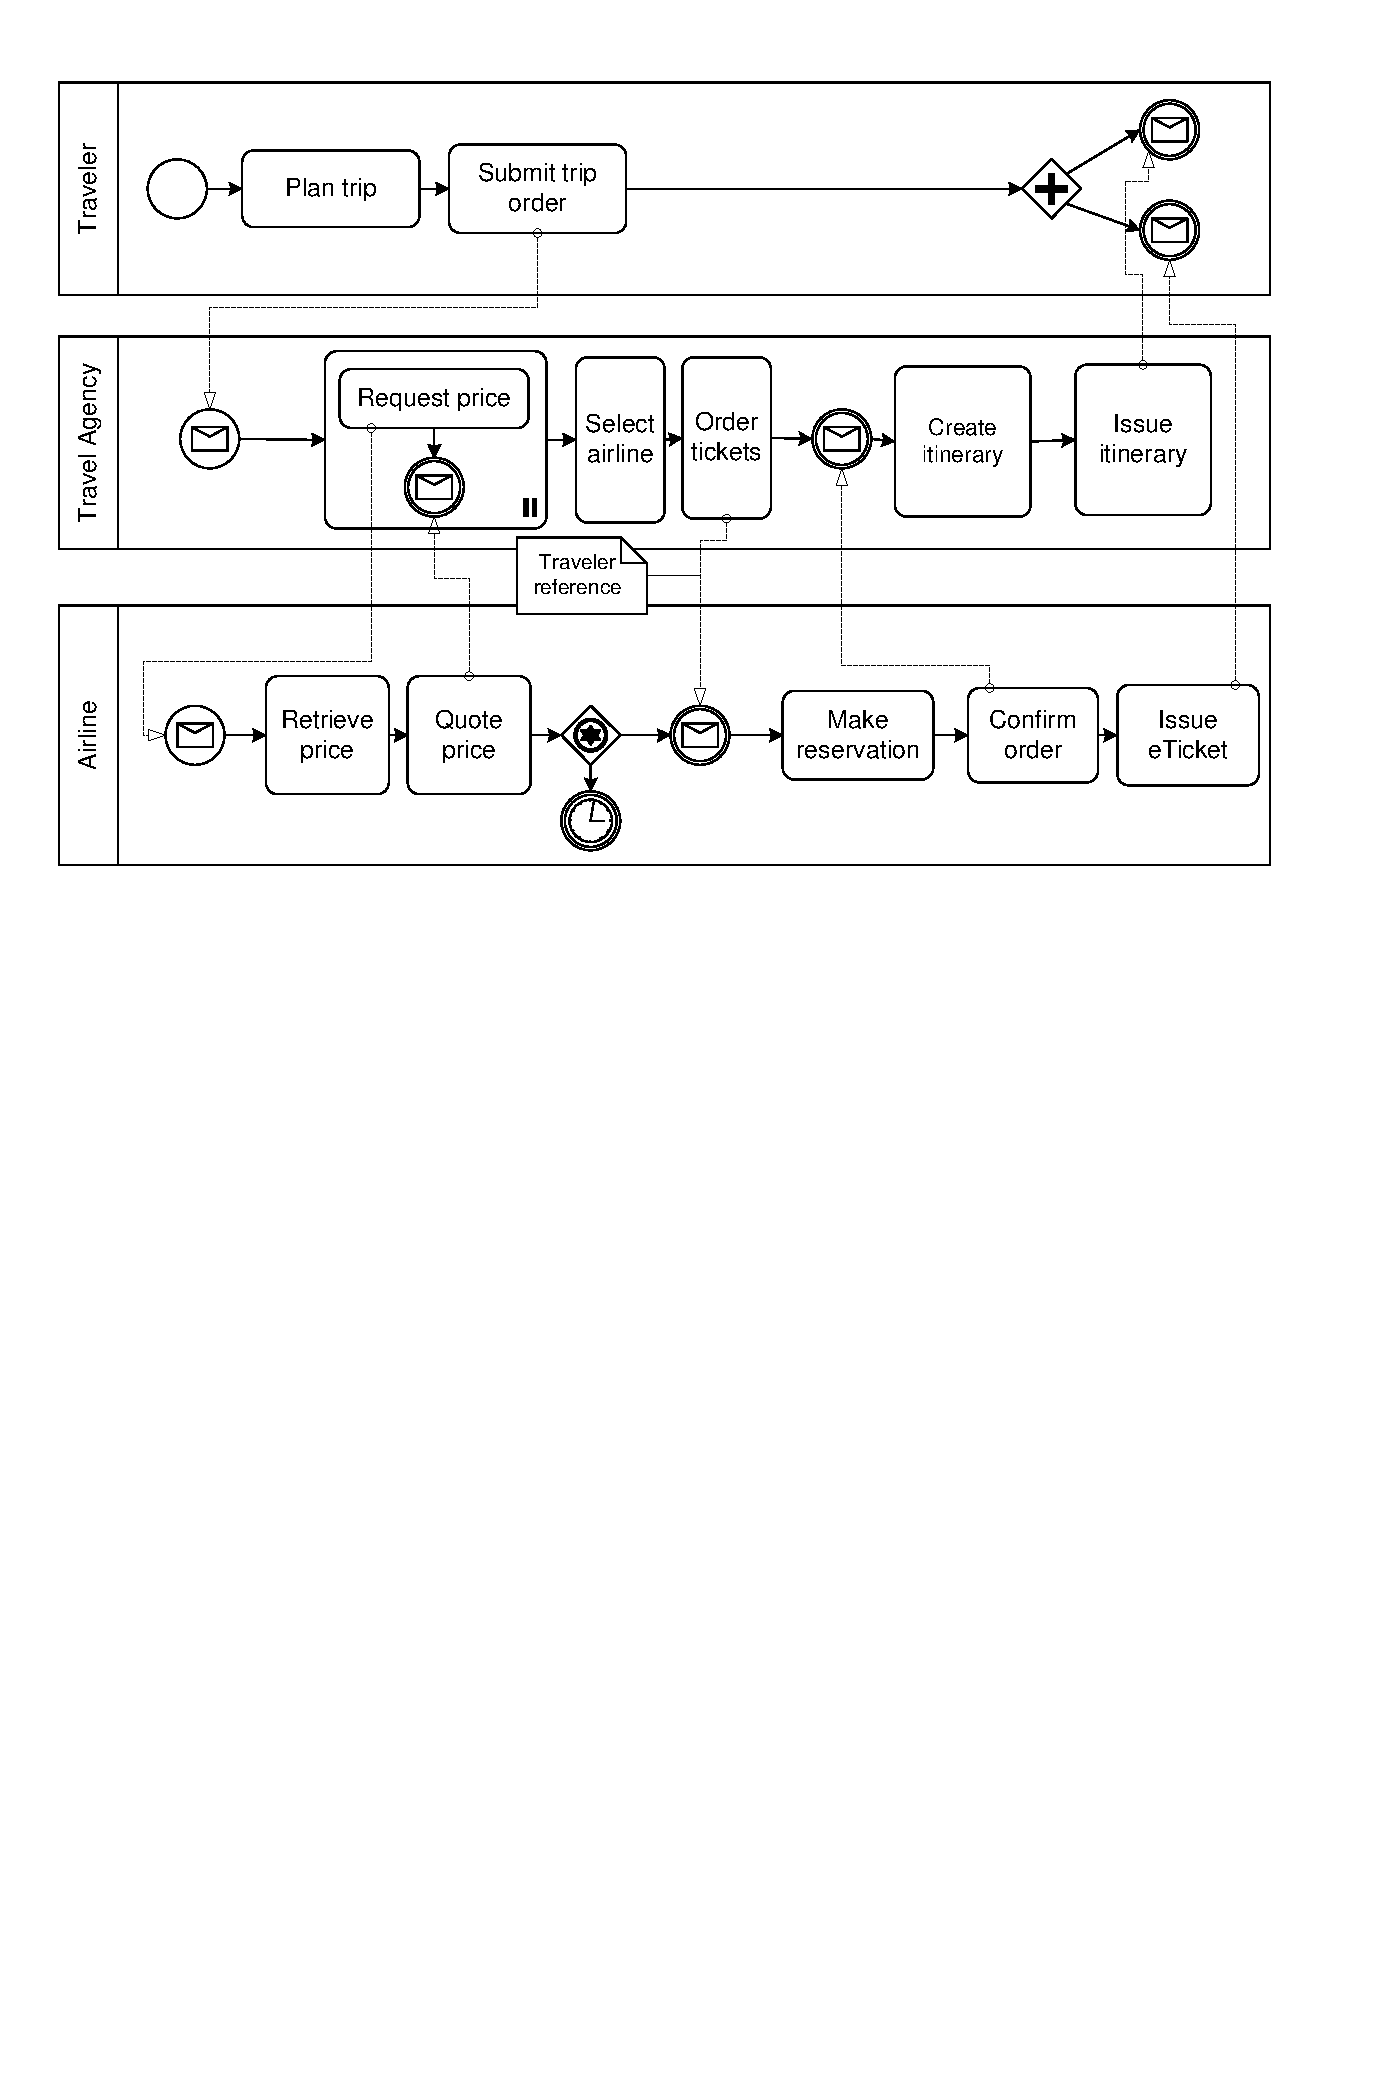
\includegraphics[width=\textwidth]{choreography.pdf}
  \caption{Beispiel-Choreographie I}
  \label{fig:AnhangsChor}
\end{figure}

\begin{landscape}
%sidewaysfigure
\begin{figure}
  \centering
  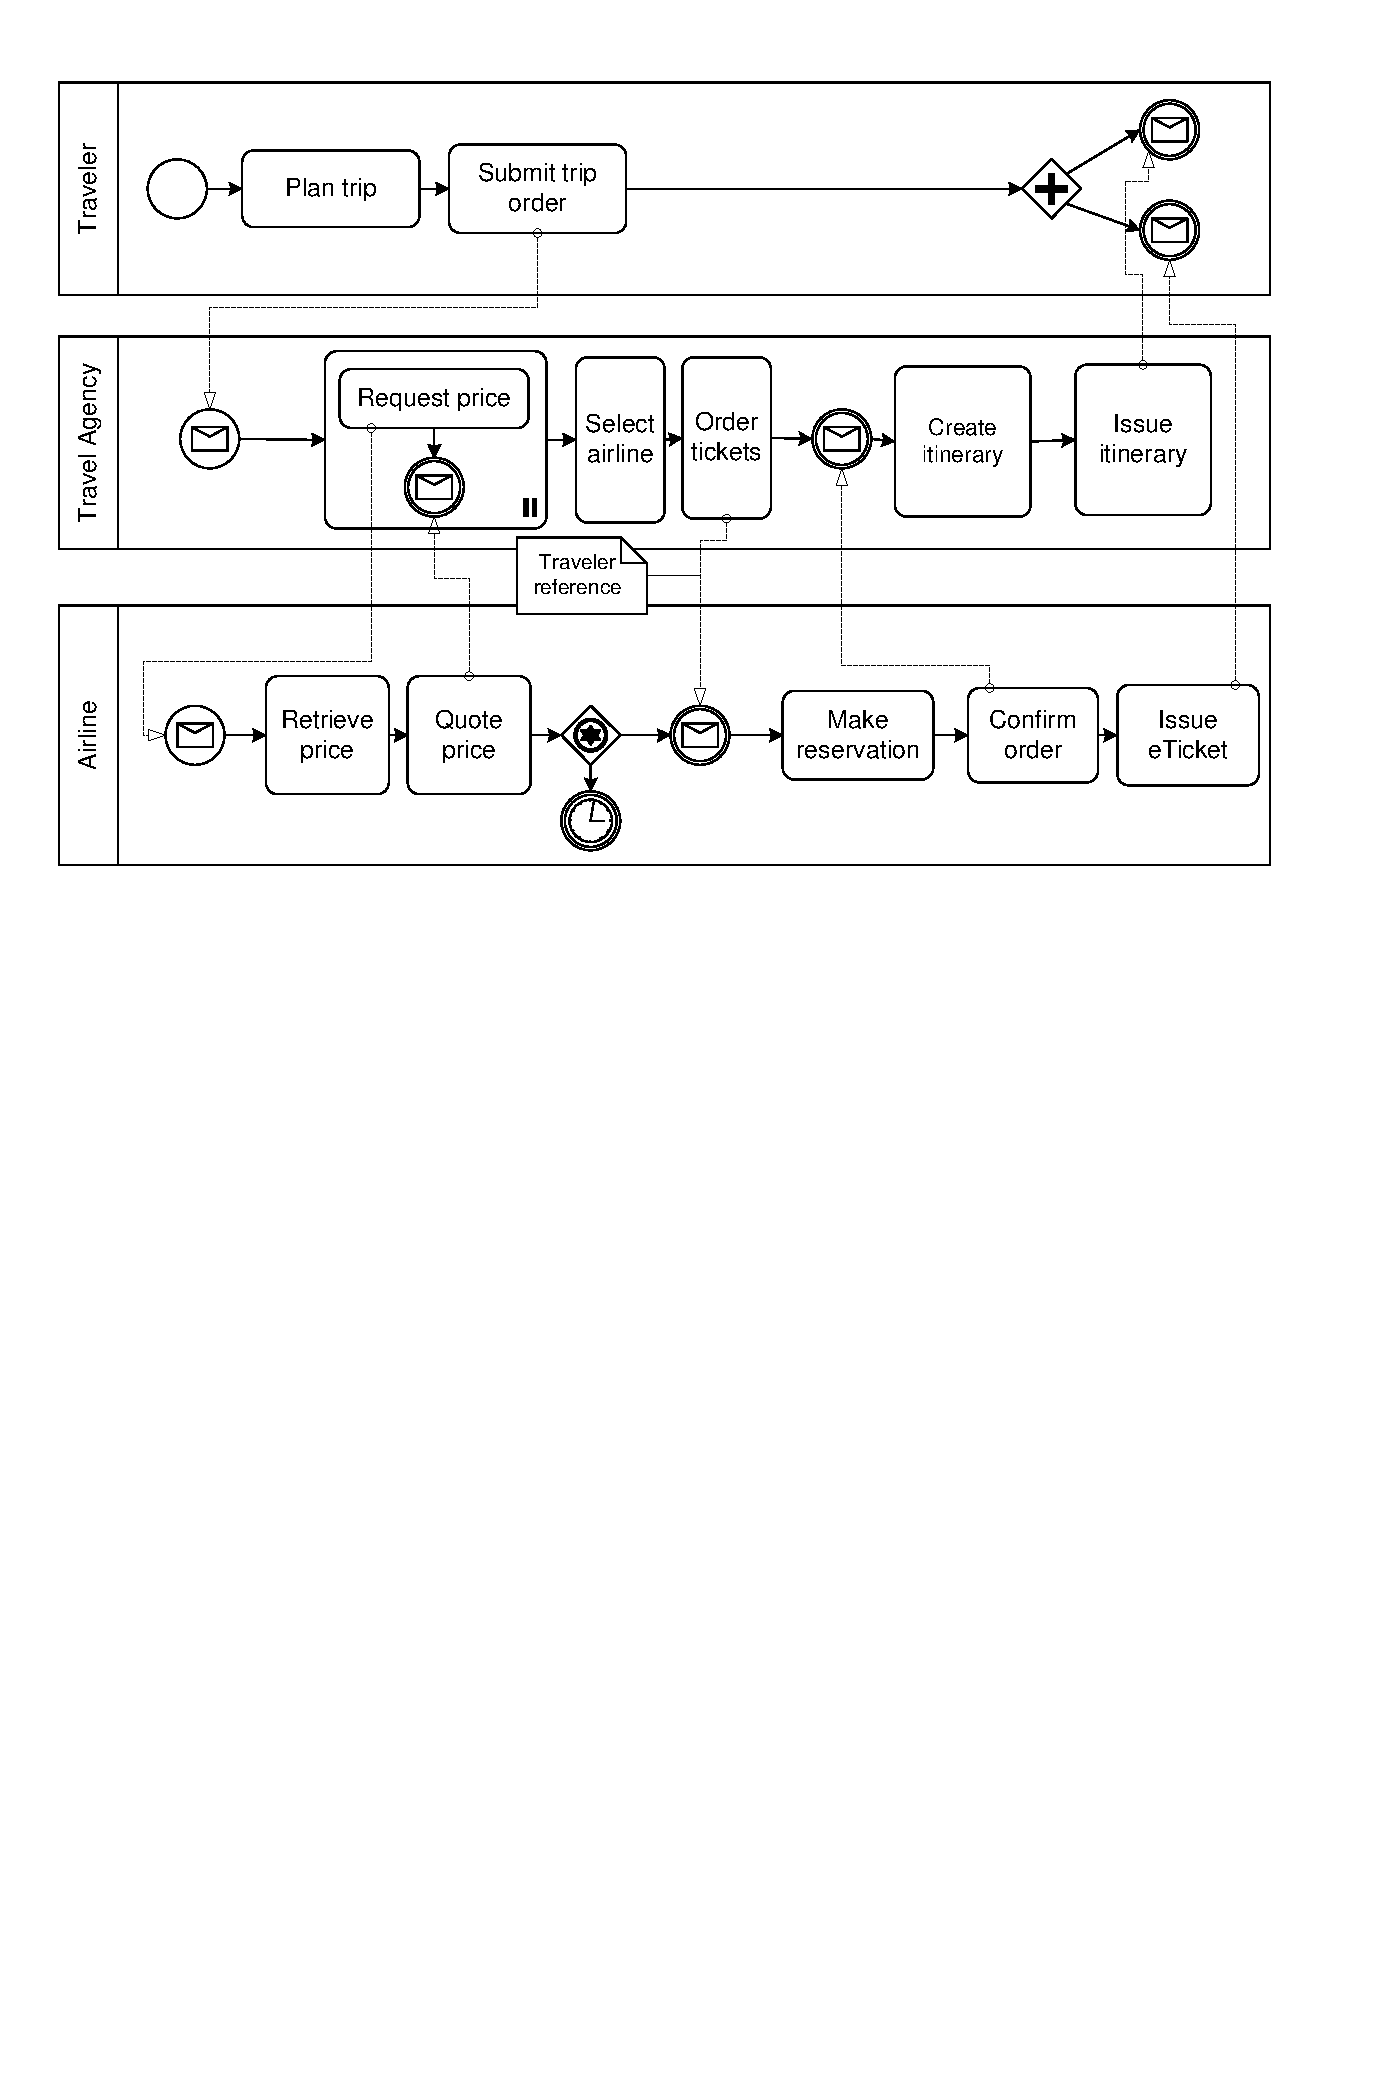
\includegraphics[width=\textwidth]{choreography.pdf}
  \caption{Beispiel-Choreographie II}
  \label{fig:AnhangsChor2}
\end{figure}
\end{landscape}


%\printindex

\printbibliography

\ifdeutsch
All links were last followed on \today.
\else
All links were last followed on \today.
\fi

\pagestyle{empty}
\renewcommand*{\chapterpagestyle}{empty}
%\Versicherung
\pagestyle{empty}
\vspace{9cm}
\begin{center}
	\begin{minipage}{11cm}
		\vspace{6cm}
		
		\textbf{\Large Declaration}\\\\
		\vspace{0.4cm}
		
		I hereby declare that the work presented in this thesis is entirely my own. 
		I did not use any other sources and references than the listed ones. I have marked all direct or indirect statements from other sources contained therein as quotations. 
		Neither this work nor significant parts of it were part of another examination procedure. I have not published this work in whole or in part before. 
		The electronic copy is consistent with all submitted copies.
		\vspace{1cm}
		
		
		
		
\hspace{2.1cm}-----------------------------------------------------------\\
\vspace{1cm} \hspace{2.1cm} place,date,signature
	\end{minipage}
\end{center}

\end{document}
